\documentclass[12pt]{article}
\usepackage[utf8]{inputenc}
\usepackage{amsmath}
\usepackage{amssymb}
\usepackage{graphicx}
\usepackage[a4paper, margin=1in]{geometry}
\usepackage{hyperref}
\usepackage{xcolor}
\usepackage{listings}

% --- Style configuration for the code block ---
\definecolor{codegreen}{rgb}{0,0.6,0}
\definecolor{codegray}{rgb}{0.5,0.5,0.5}
\definecolor{codepurple}{rgb}{0.58,0,0.82}
\definecolor{backcolour}{rgb}{0.95,0.95,0.92}

\lstdefinestyle{mystyle}{
    backgroundcolor=\color{backcolour},   
    commentstyle=\color{codegreen},
    keywordstyle=\color{magenta},
    numberstyle=\tiny\color{codegray},
    stringstyle=\color{codepurple},
    basicstyle=\ttfamily\footnotesize,
    breakatwhitespace=false,         
    breaklines=true,                 
    captionpos=b,                    
    keepspaces=true,                 
    numbers=left,                    
    numbersep=5pt,                  
    showspaces=false,                
    showstringspaces=false,
    showtabs=false,                  
    tabsize=2
}

\lstset{style=mystyle}

\title{Visualizing Probability: A Monte Carlo Simulation of Expected Value and the Law of Large Numbers}
\author{Tashfeen Omran}
\date{October 23, 2025}

\begin{document}

\maketitle

\begin{abstract}
This document explores the fundamental statistical concepts of Expected Value (EV), variance, and the Law of Large Numbers (LLN) through a series of Monte Carlo simulations. By simulating a simple coin flip game with positive, negative, and neutral expected values across a growing number of trials, we can visually demonstrate how short-term randomness converges to long-term predictability. The simulations serve as a practical bridge between abstract probability theory and tangible outcomes.
\end{abstract}

\tableofcontents
\clearpage

% --- SECTION 1: INTRODUCTION & MATHEMATICAL FOUNDATION ---
\section{Introduction and Mathematical Foundation}

In the study of probability, predicting the outcome of a single random event is impossible. However, over a large number of repetitions, patterns emerge from the chaos. This phenomenon is the bedrock of the insurance industry, casino operations, and quantitative finance. This experiment uses a Monte Carlo method which is a computational technique that relies on repeated random sampling to simulate a coin flip game and observe these principles in action.

\subsection{Expected Value (EV)}
The Expected Value (EV) is the long-run average value of a random variable. It represents the mean outcome if an experiment were repeated an infinite number of times. It is calculated by summing the products of each possible outcome and its probability.

The general formula is:
\[
E[X] = \sum_{i=1}^{n} x_i P(x_i)
\]
Where $x_i$ is the value of outcome $i$ and $P(x_i)$ is its probability.

\subsection{Variance and Standard Deviation}
Variance ($\sigma^2$) measures the dispersion of a set of outcomes around their mean (the EV). A low variance indicates that the outcomes tend to be very close to the expected value, while a high variance indicates that the outcomes are spread out over a wider range.

The formula for variance is:
\[
\sigma^2 = E[(X - \mu)^2] = \sum_{i=1}^{n} (x_i - \mu)^2 P(x_i)
\]
Where $\mu$ is the expected value $E[X]$.

\subsection{The Law of Large Numbers (LLN)}
The Law of Large Numbers (LLN) is a core theorem of probability theory which states that as the size of a sample taken from a population increases, the sample mean ($\bar{X}_n$) will converge to the theoretical expected value ($\mu$).
\[
\bar{X}_n \to \mu \quad \text{as} \quad n \to \infty
\]
This is the principle that ensures profitability in games of chance where a statistical edge exists. It does not state that results will be "evened out" by future outcomes, but rather that the impact of early-stage variance becomes diluted as the number of trials ($n$) grows.

\subsection{Variance of the Sample Mean}
The most crucial concept for understanding our simulations is how the variance of the \textbf{average outcome} behaves. If a single game has a variance of $\sigma^2$, the variance of the average profit over $n$ games is:
\[
\text{Var}(\bar{X}_n) = \frac{\sigma^2}{n}
\]
This formula is the mathematical engine behind the LLN. It shows that as $n$ increases, the variance of the average outcome decreases, meaning the average becomes a more reliable estimate of the true EV. Our confidence in the outcome grows with the sample size.

% --- SECTION 2: POSITIVE EV SIMULATION ---
\section{Case Study 1: The Positive EV Game}
In this scenario, the game is structured to be profitable for the player in the long run.

\subsection{Game Rules and Calculation}
\begin{itemize}
    \item \textbf{Cost to Play:} \$1.00
    \item \textbf{Heads Payout:} \$3.00 (Net profit: \$2.00)
    \item \textbf{Tails Payout:} \$0.00 (Net loss: \$1.00)
\end{itemize}
The Expected Value per flip is calculated as:
\[
EV = (0.5 \times \$2.00) + (0.5 \times -\$1.00) = \$1.00 - \$0.50 = \boldsymbol{+\$0.50}
\]
For every flip, we expect to make an average profit of 50 cents. The variance for a single game is $\sigma^2 = 2.25$.

\subsection{Simulation Results}
What follows is a series of simulations with an increasing number of flips. We expect the cumulative profit paths to be highly erratic at first but gradually converge toward the theoretical profit line (a slope of +0.50 per flip).

\subsubsection{1 and 5 Flips}
With a tiny sample size, the outcome is governed entirely by chance. The LLN has no power here. A player is very likely to lose money despite the positive EV, as shown by the wide spread of outcomes. The variance is at its highest.

\begin{figure}[h!]
\centering
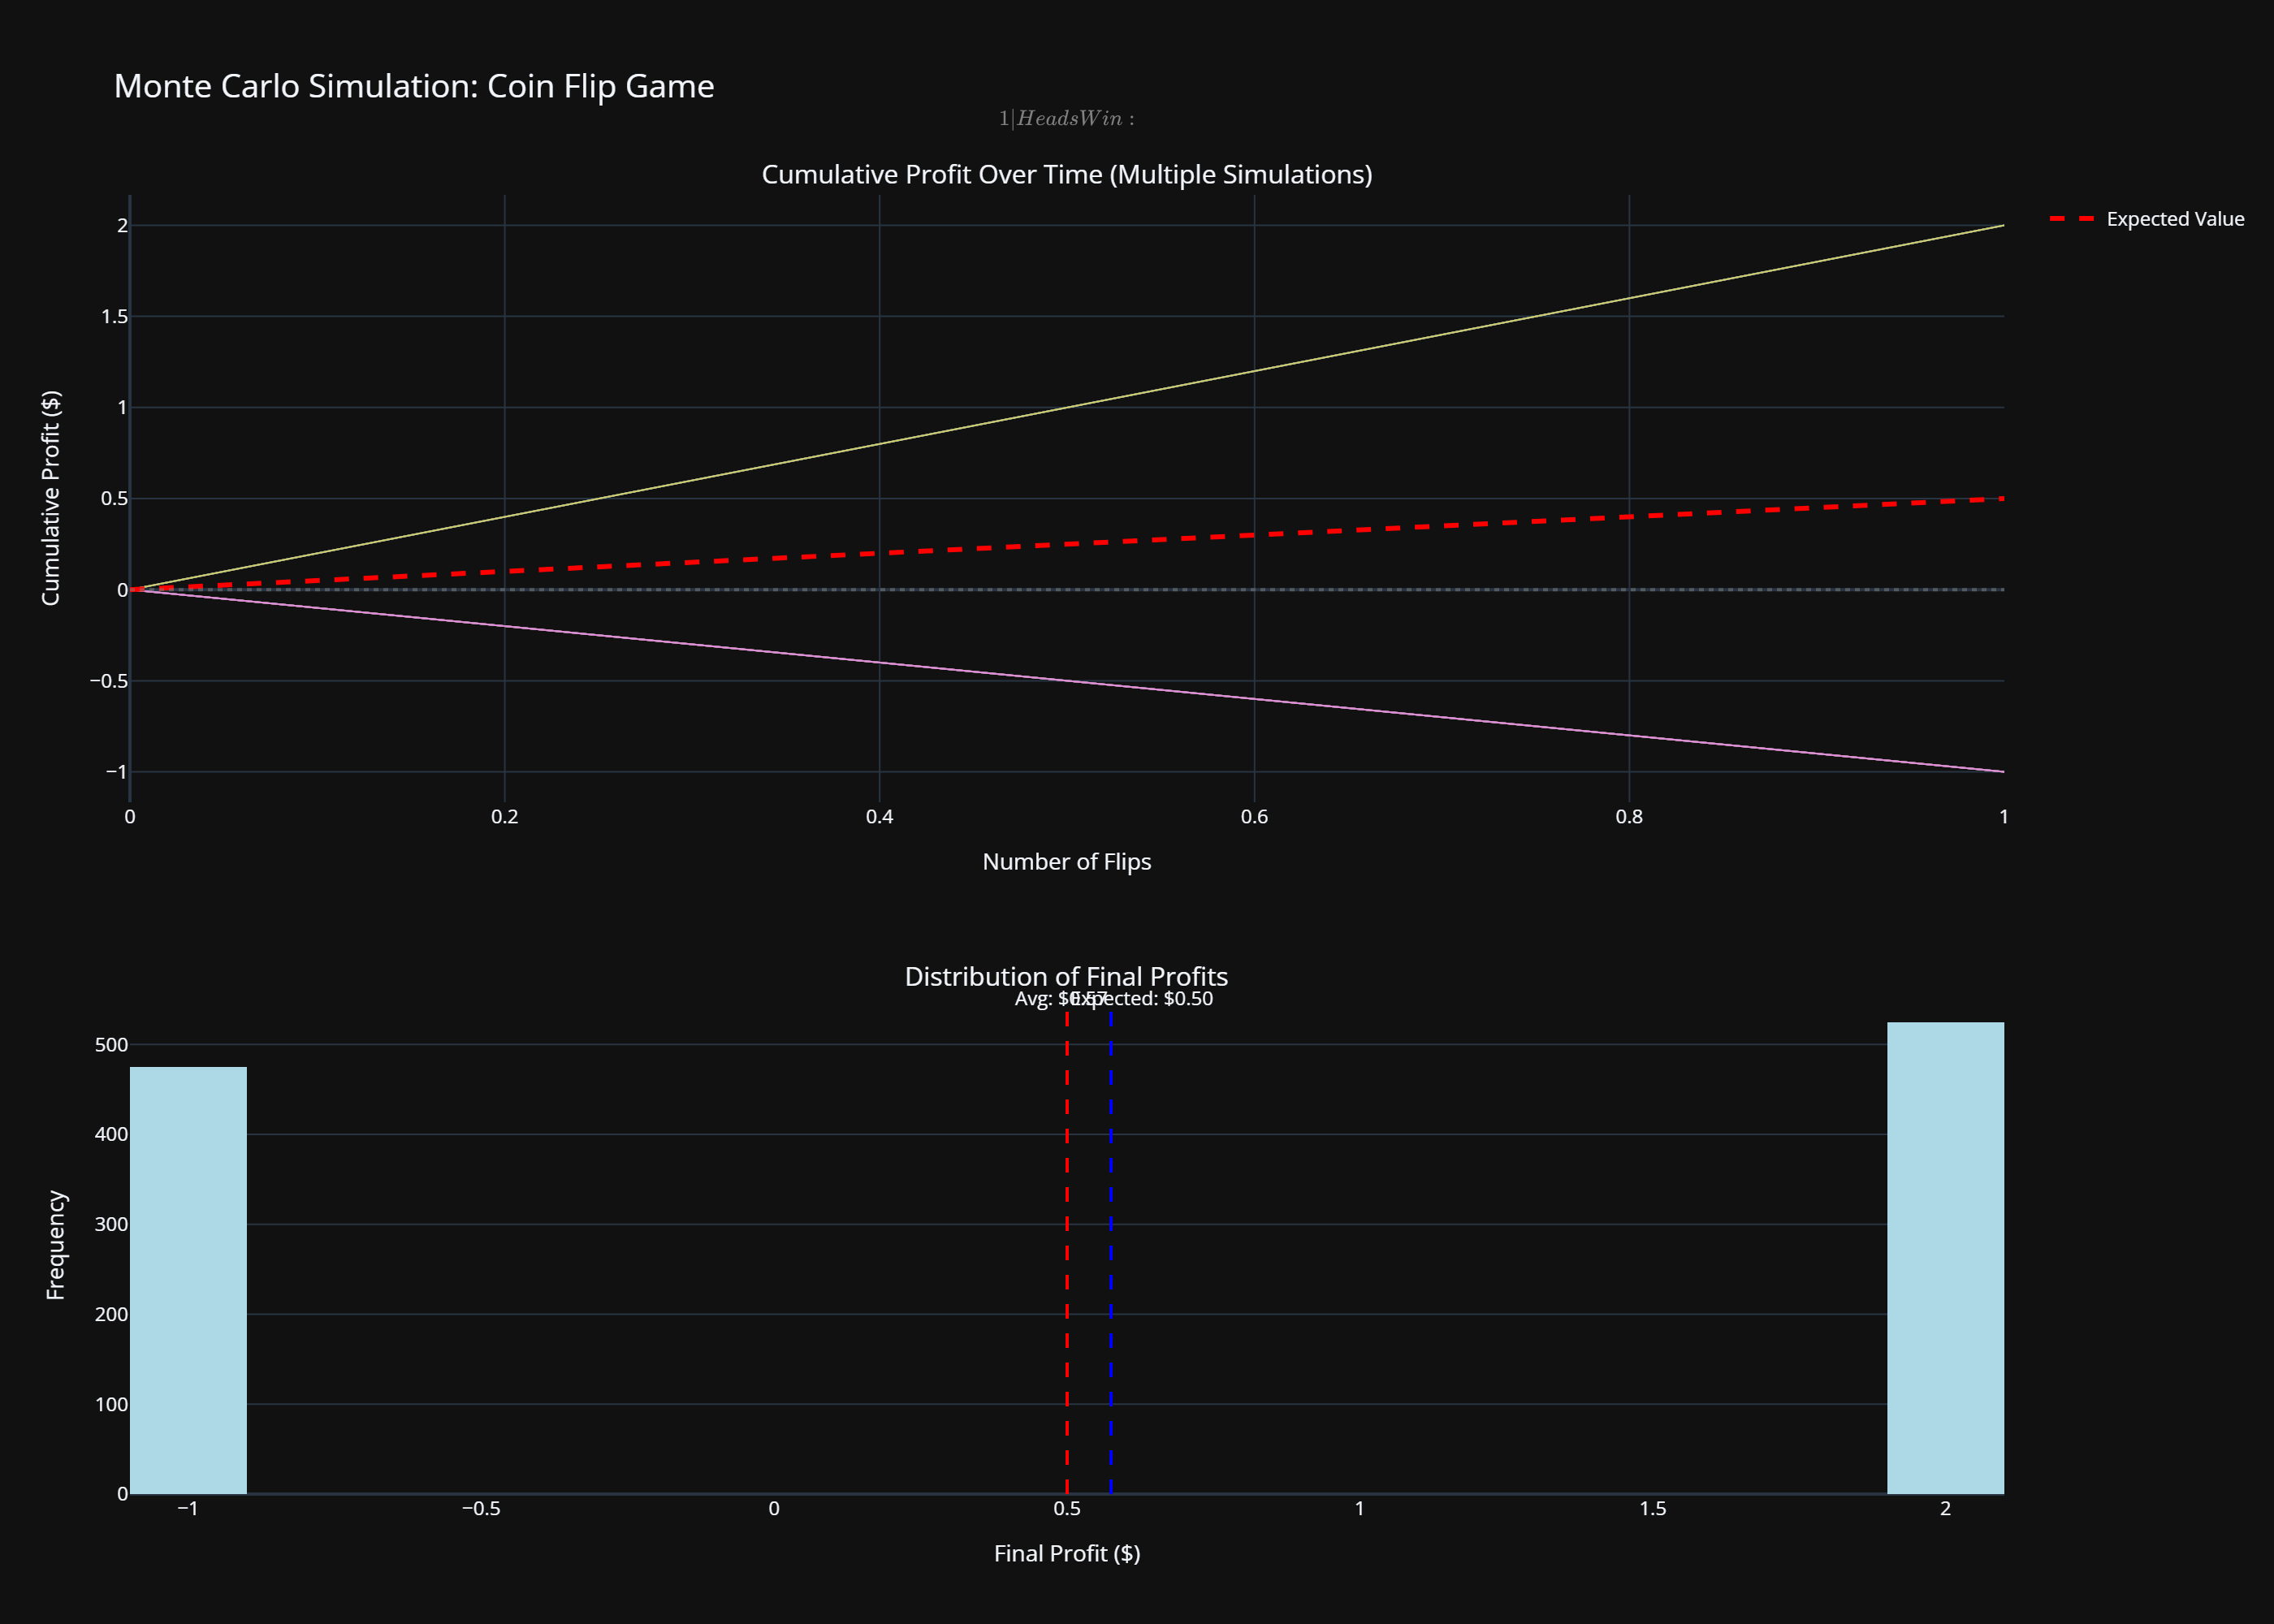
\includegraphics[width=0.8\textwidth]{+ev/1+ev.png}
\caption{Simulation with 1 flip (+EV). Outcome is binary: +\$2 or -\$1.}
\end{figure}

\begin{figure}[h!]
\centering
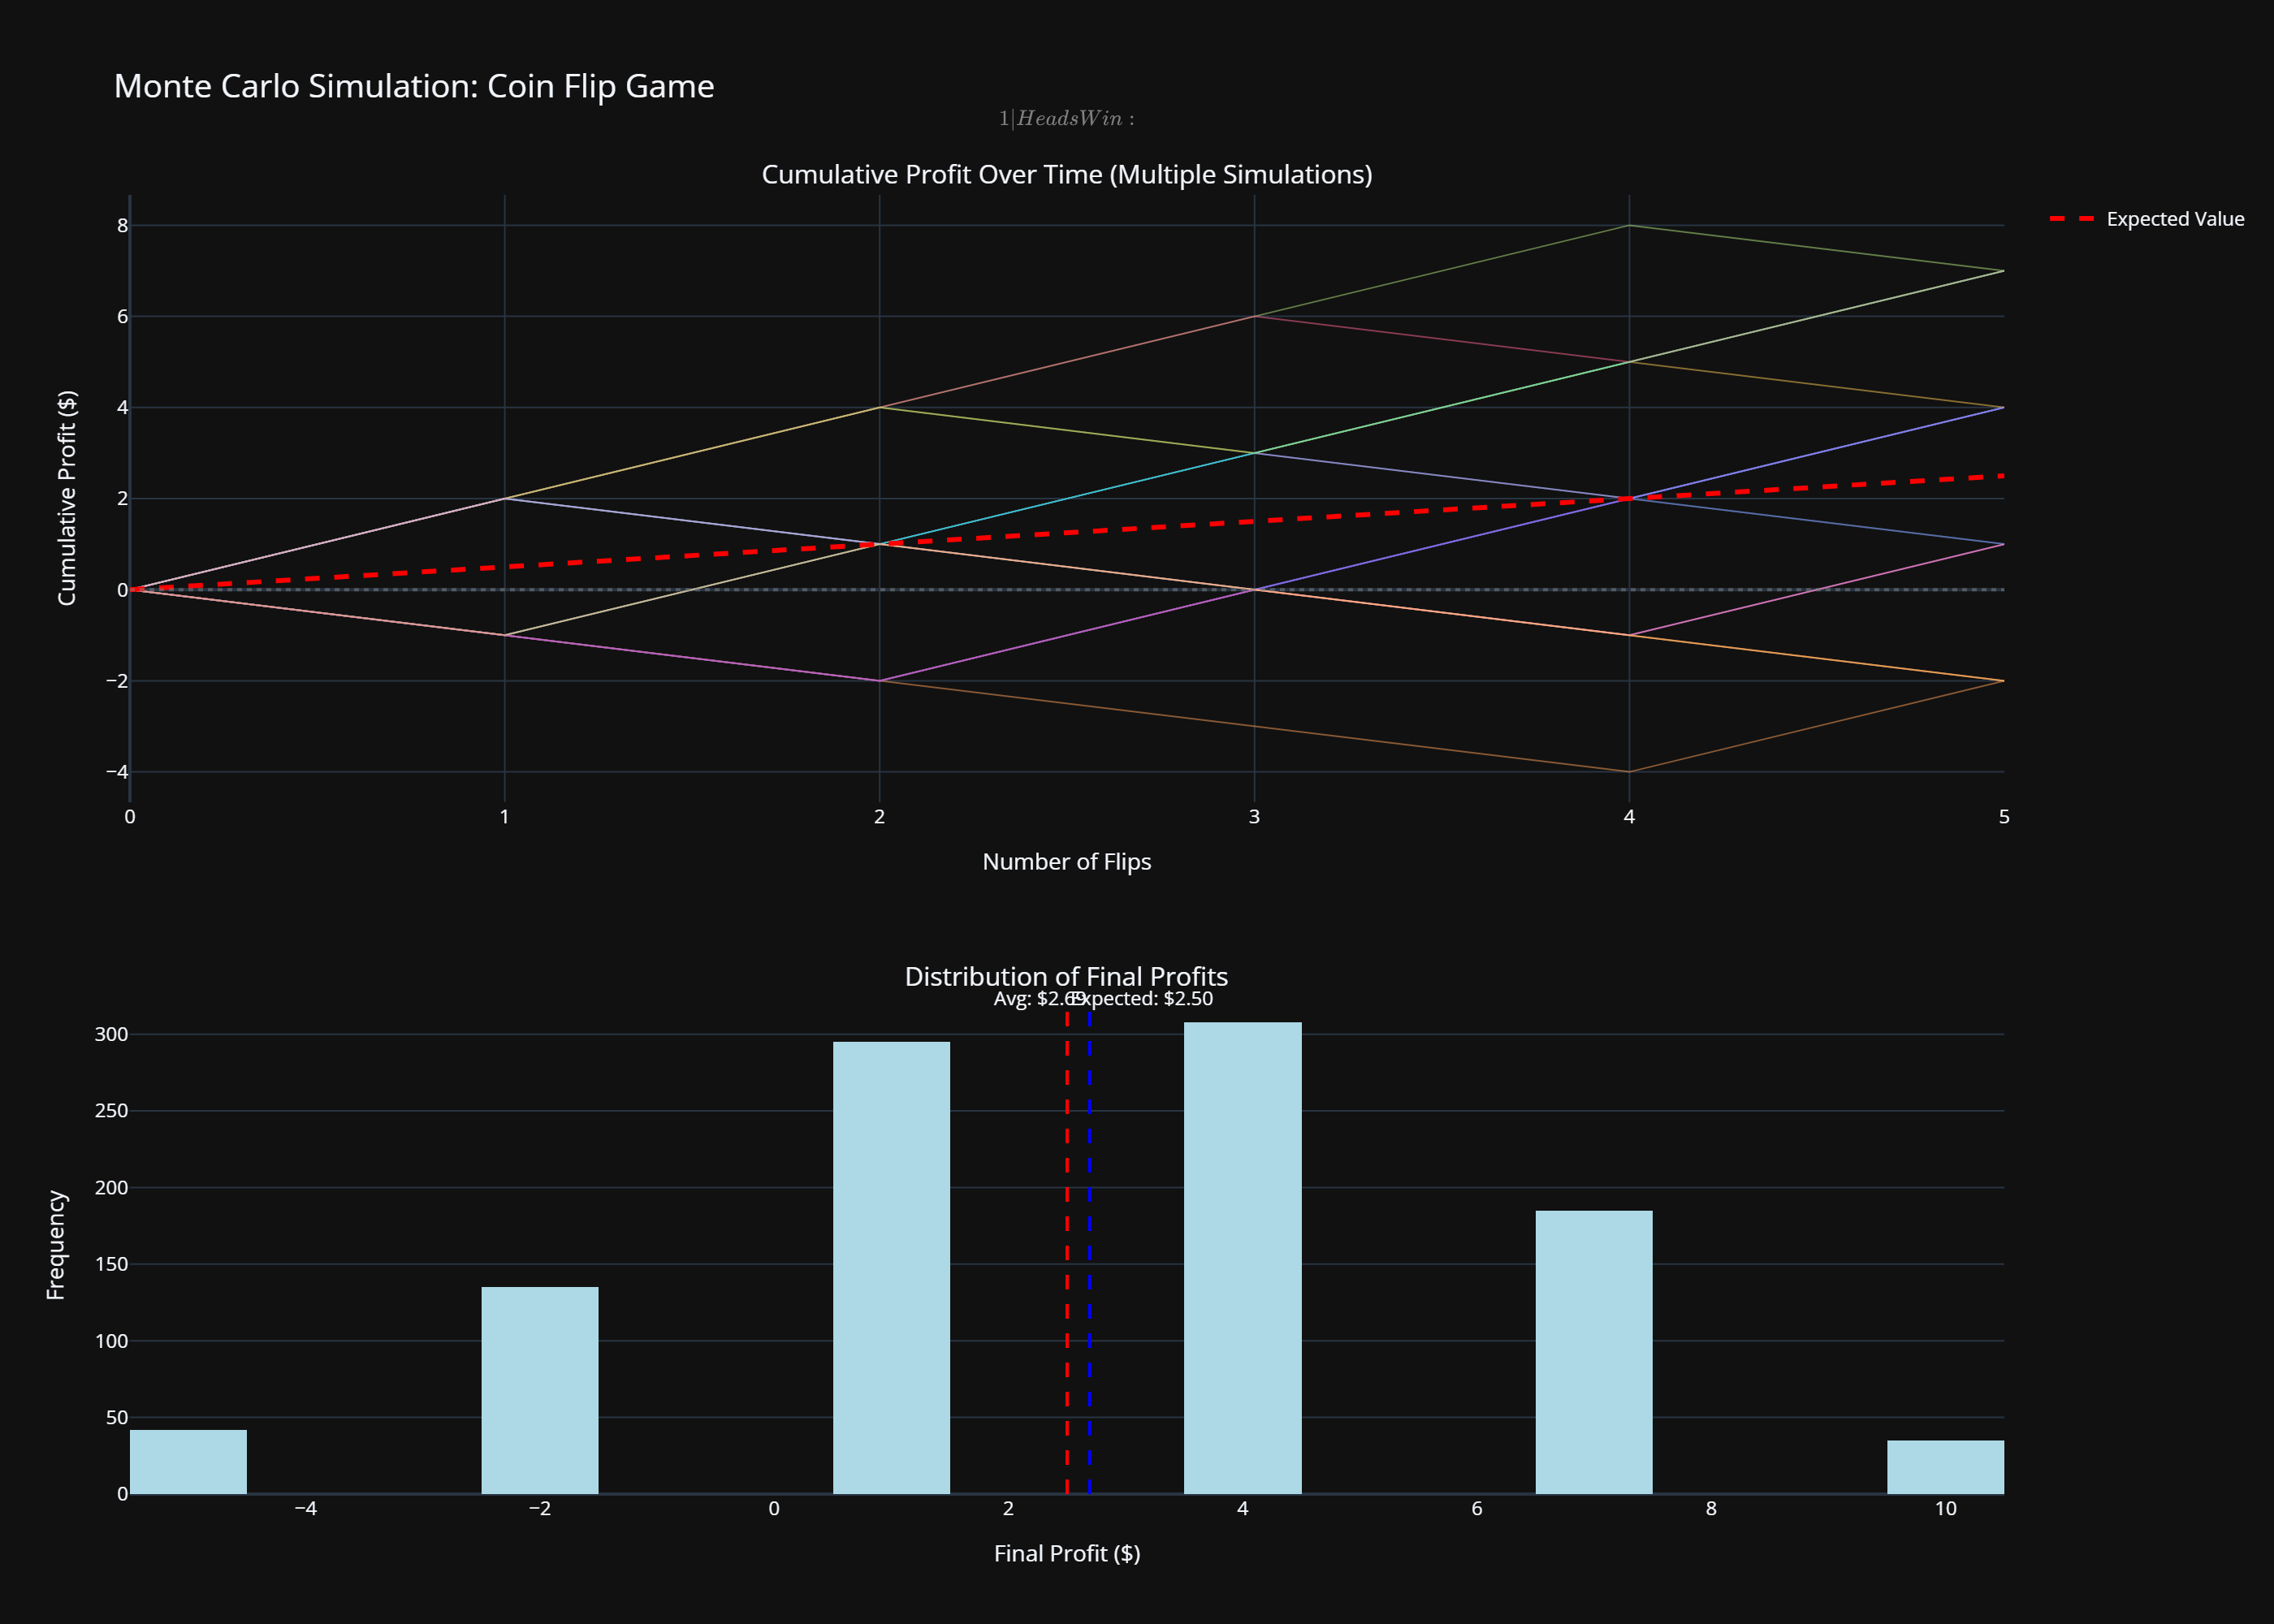
\includegraphics[width=0.8\textwidth]{+ev/5+ev.png}
\caption{Simulation with 5 flips (+EV). High variance; final profit is unpredictable.}
\end{figure}
\clearpage

\subsubsection{20 and 100 Flips}
As we increase the flips, a trend begins to emerge. While many individual simulations still deviate significantly, their collective behavior starts to drift upwards, closer to the theoretical EV line. The probability of being profitable increases.

\begin{figure}[h!]
\centering
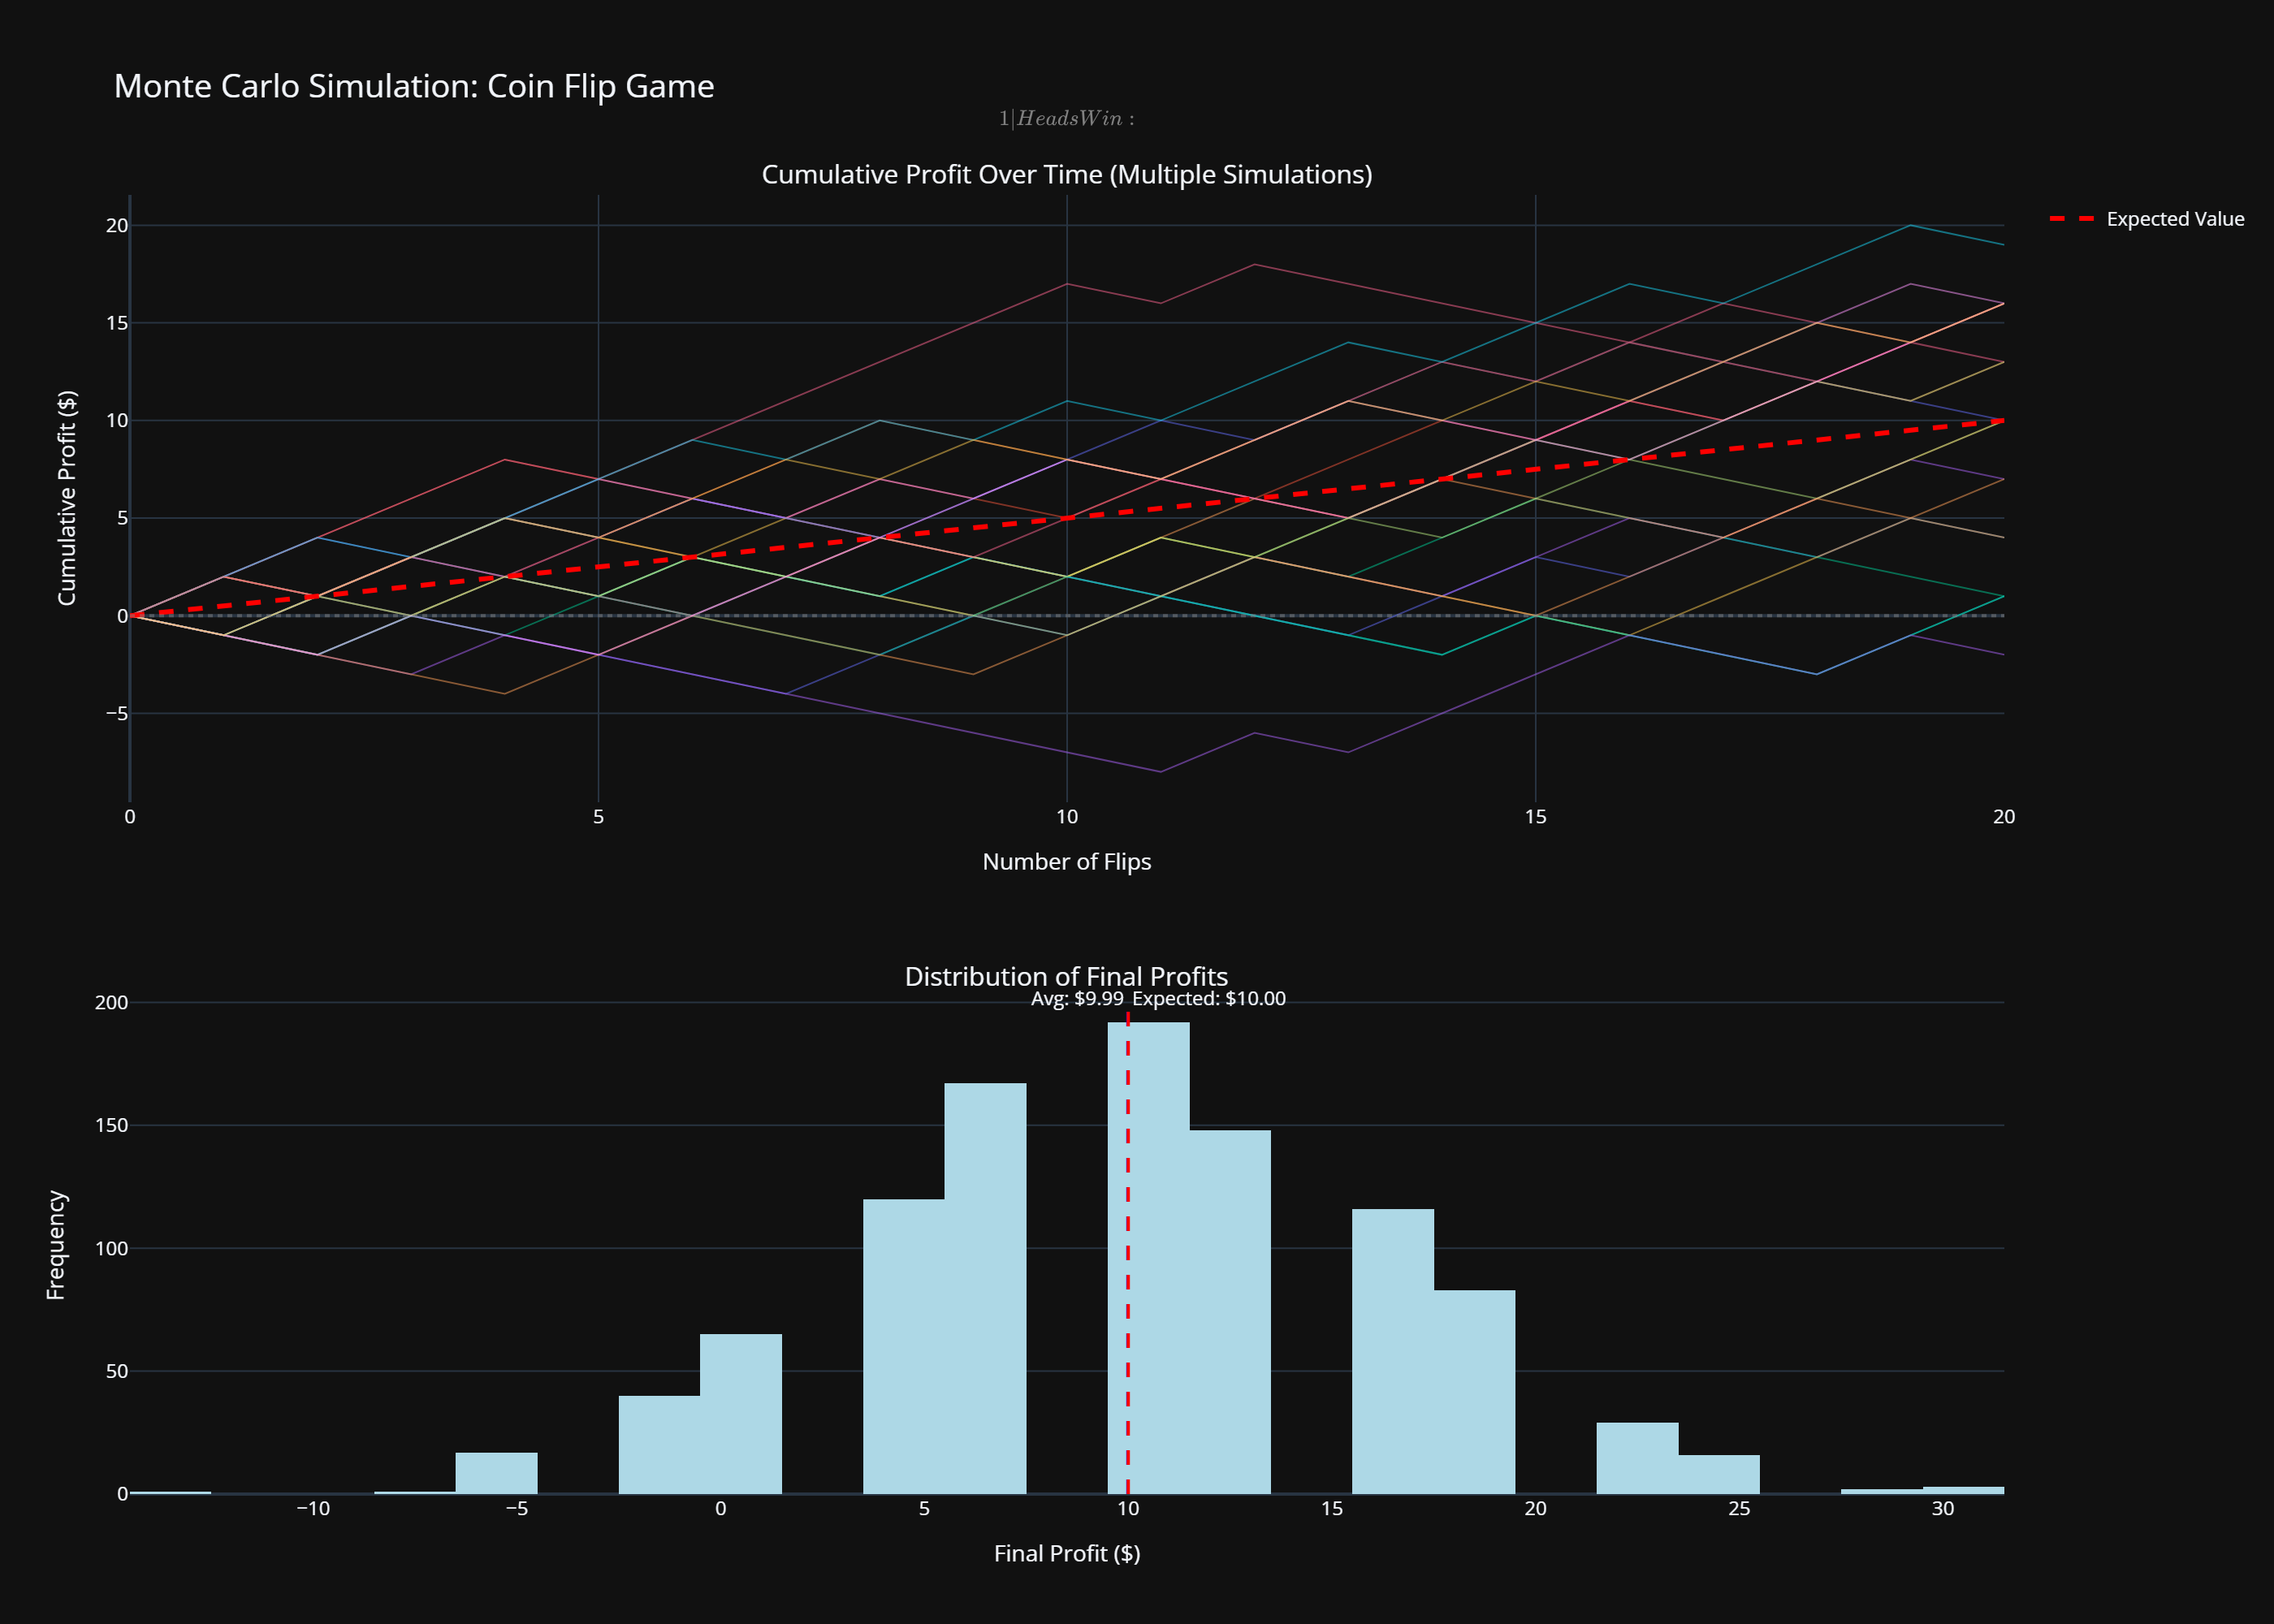
\includegraphics[width=0.8\textwidth]{+ev/20+ev.png}
\caption{Simulation with 20 flips (+EV).}
\end{figure}

\begin{figure}[h!]
\centering
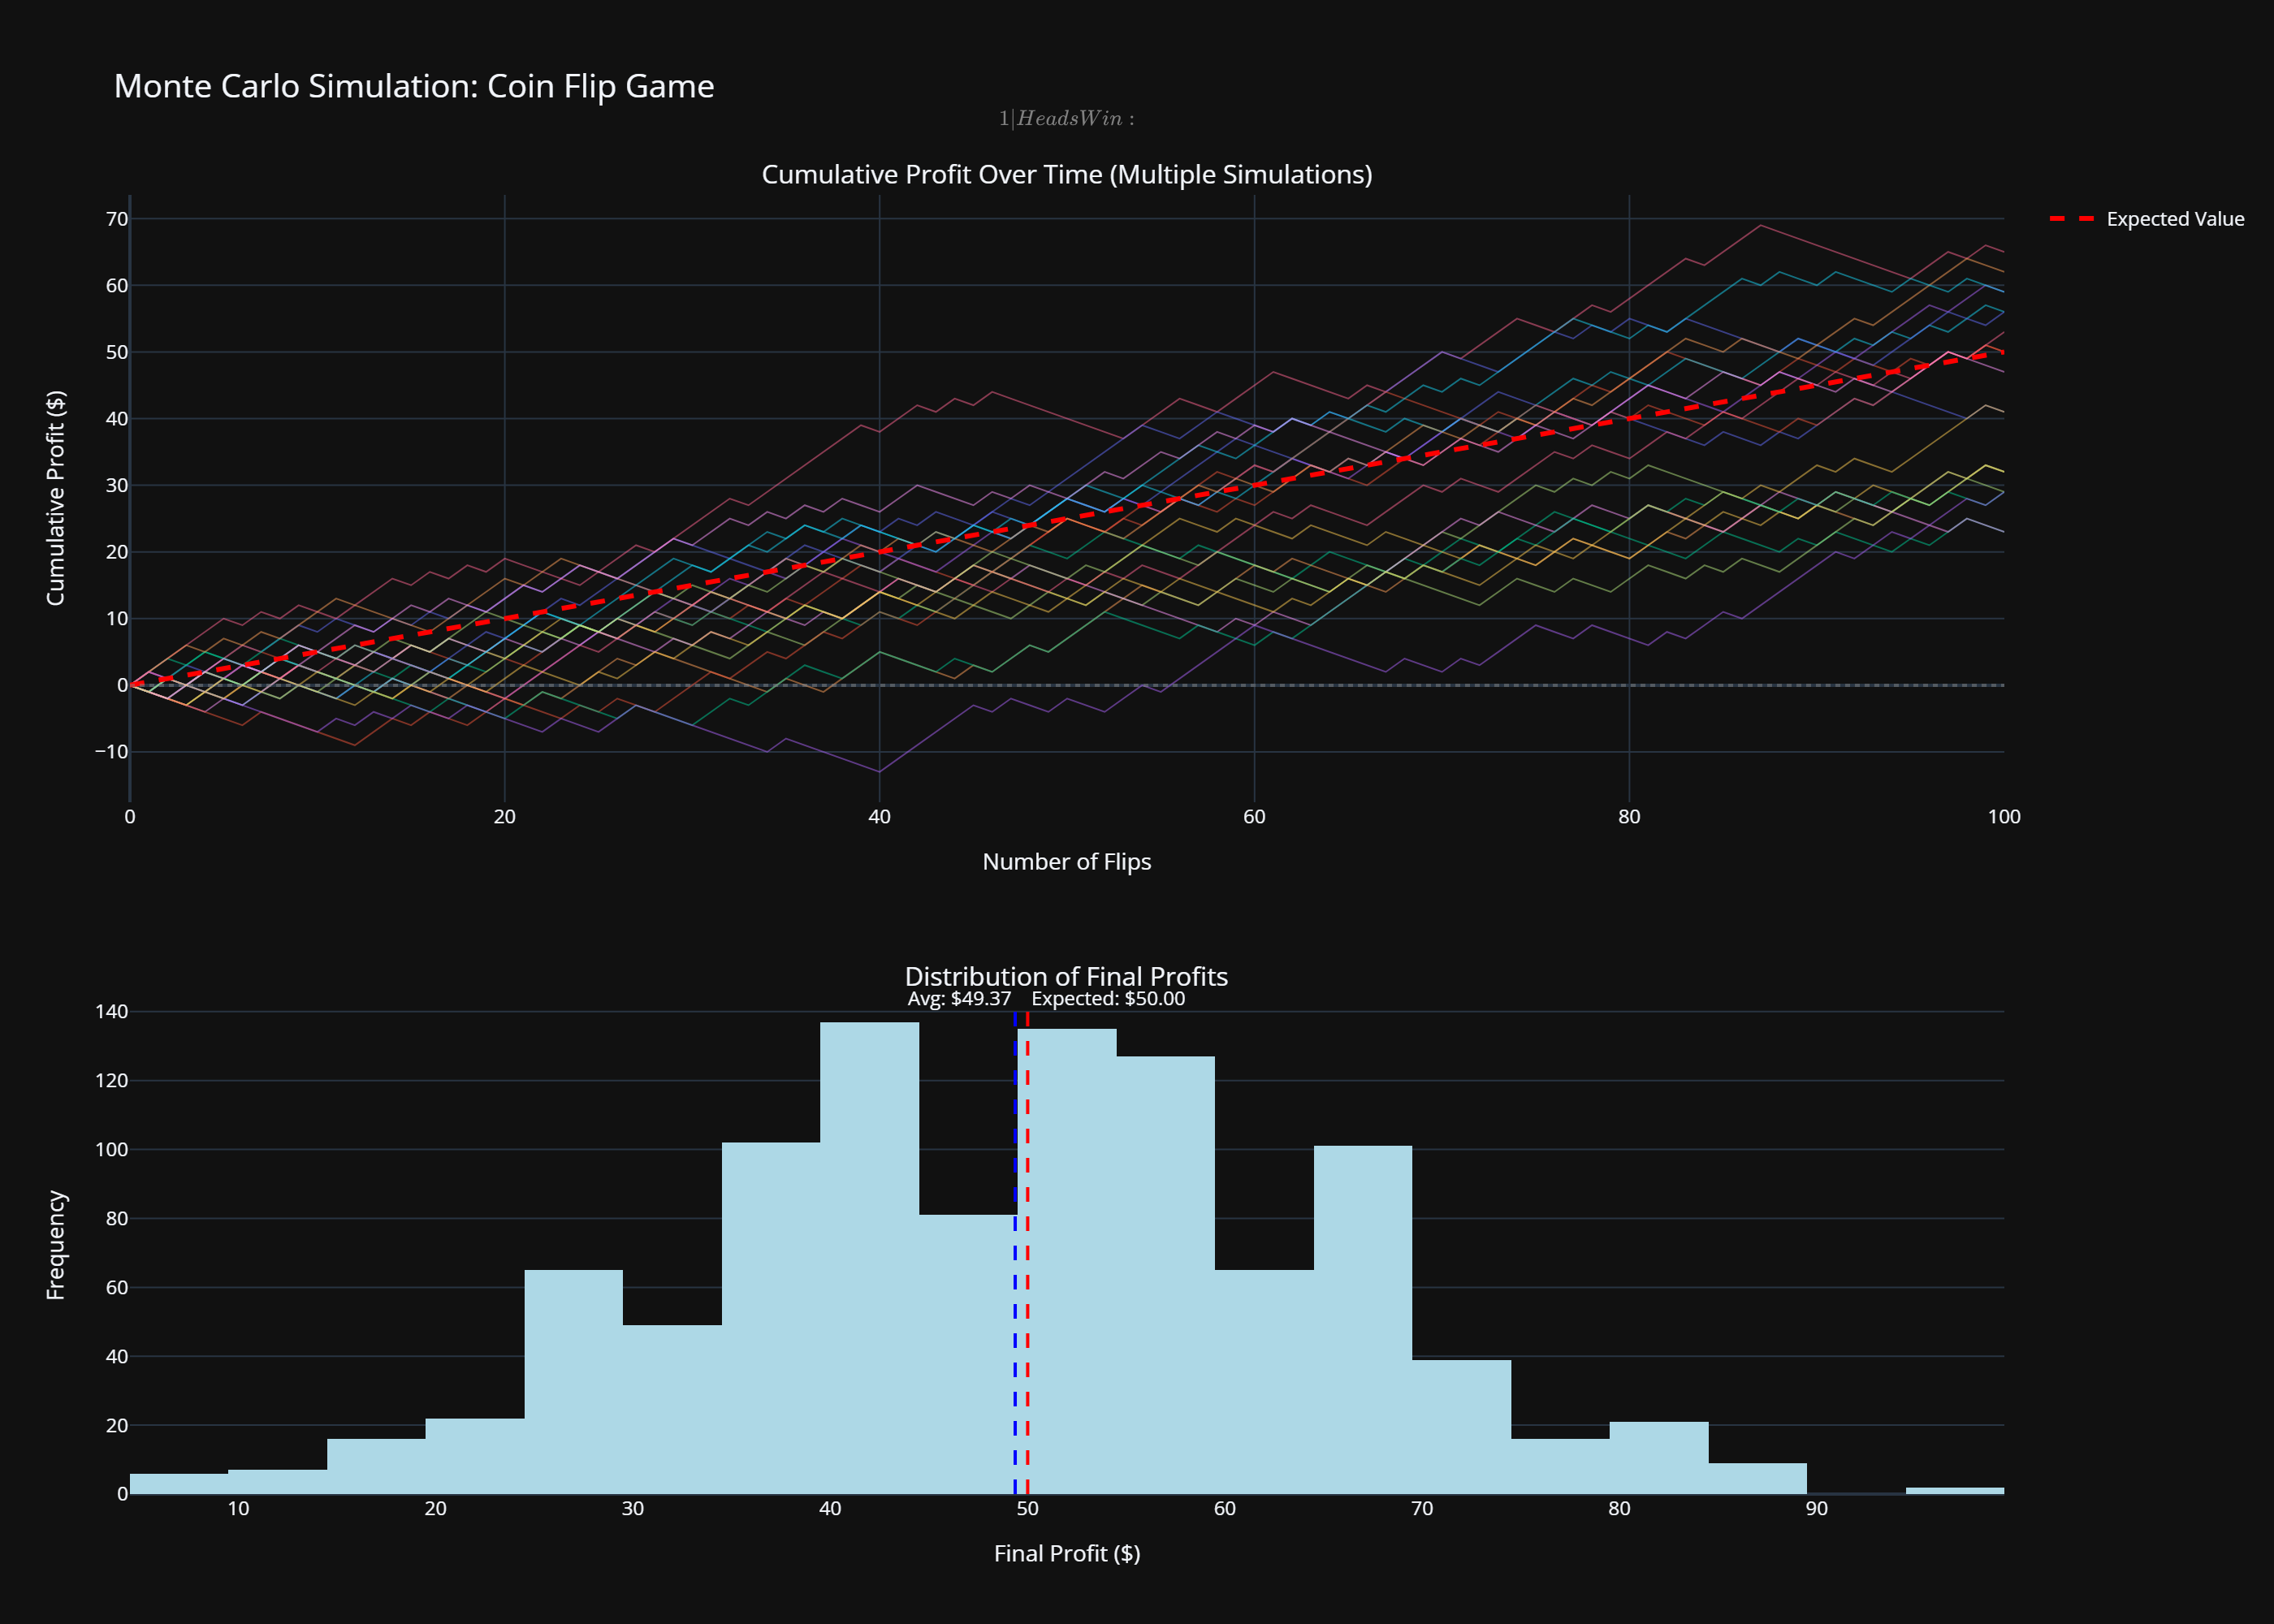
\includegraphics[width=0.8\textwidth]{+ev/100+ev.png}
\caption{Simulation with 100 flips (+EV). The upward trend is becoming clearer.}
\end{figure}
\clearpage

\subsubsection{500 and 1,000 Flips}
At this stage, the Law of Large Numbers is taking hold. The cumulative profit paths are less erratic and begin to cluster more tightly around the EV line. The histogram of final profits narrows, showing that outcomes are becoming more predictable.

\begin{figure}[h!]
\centering
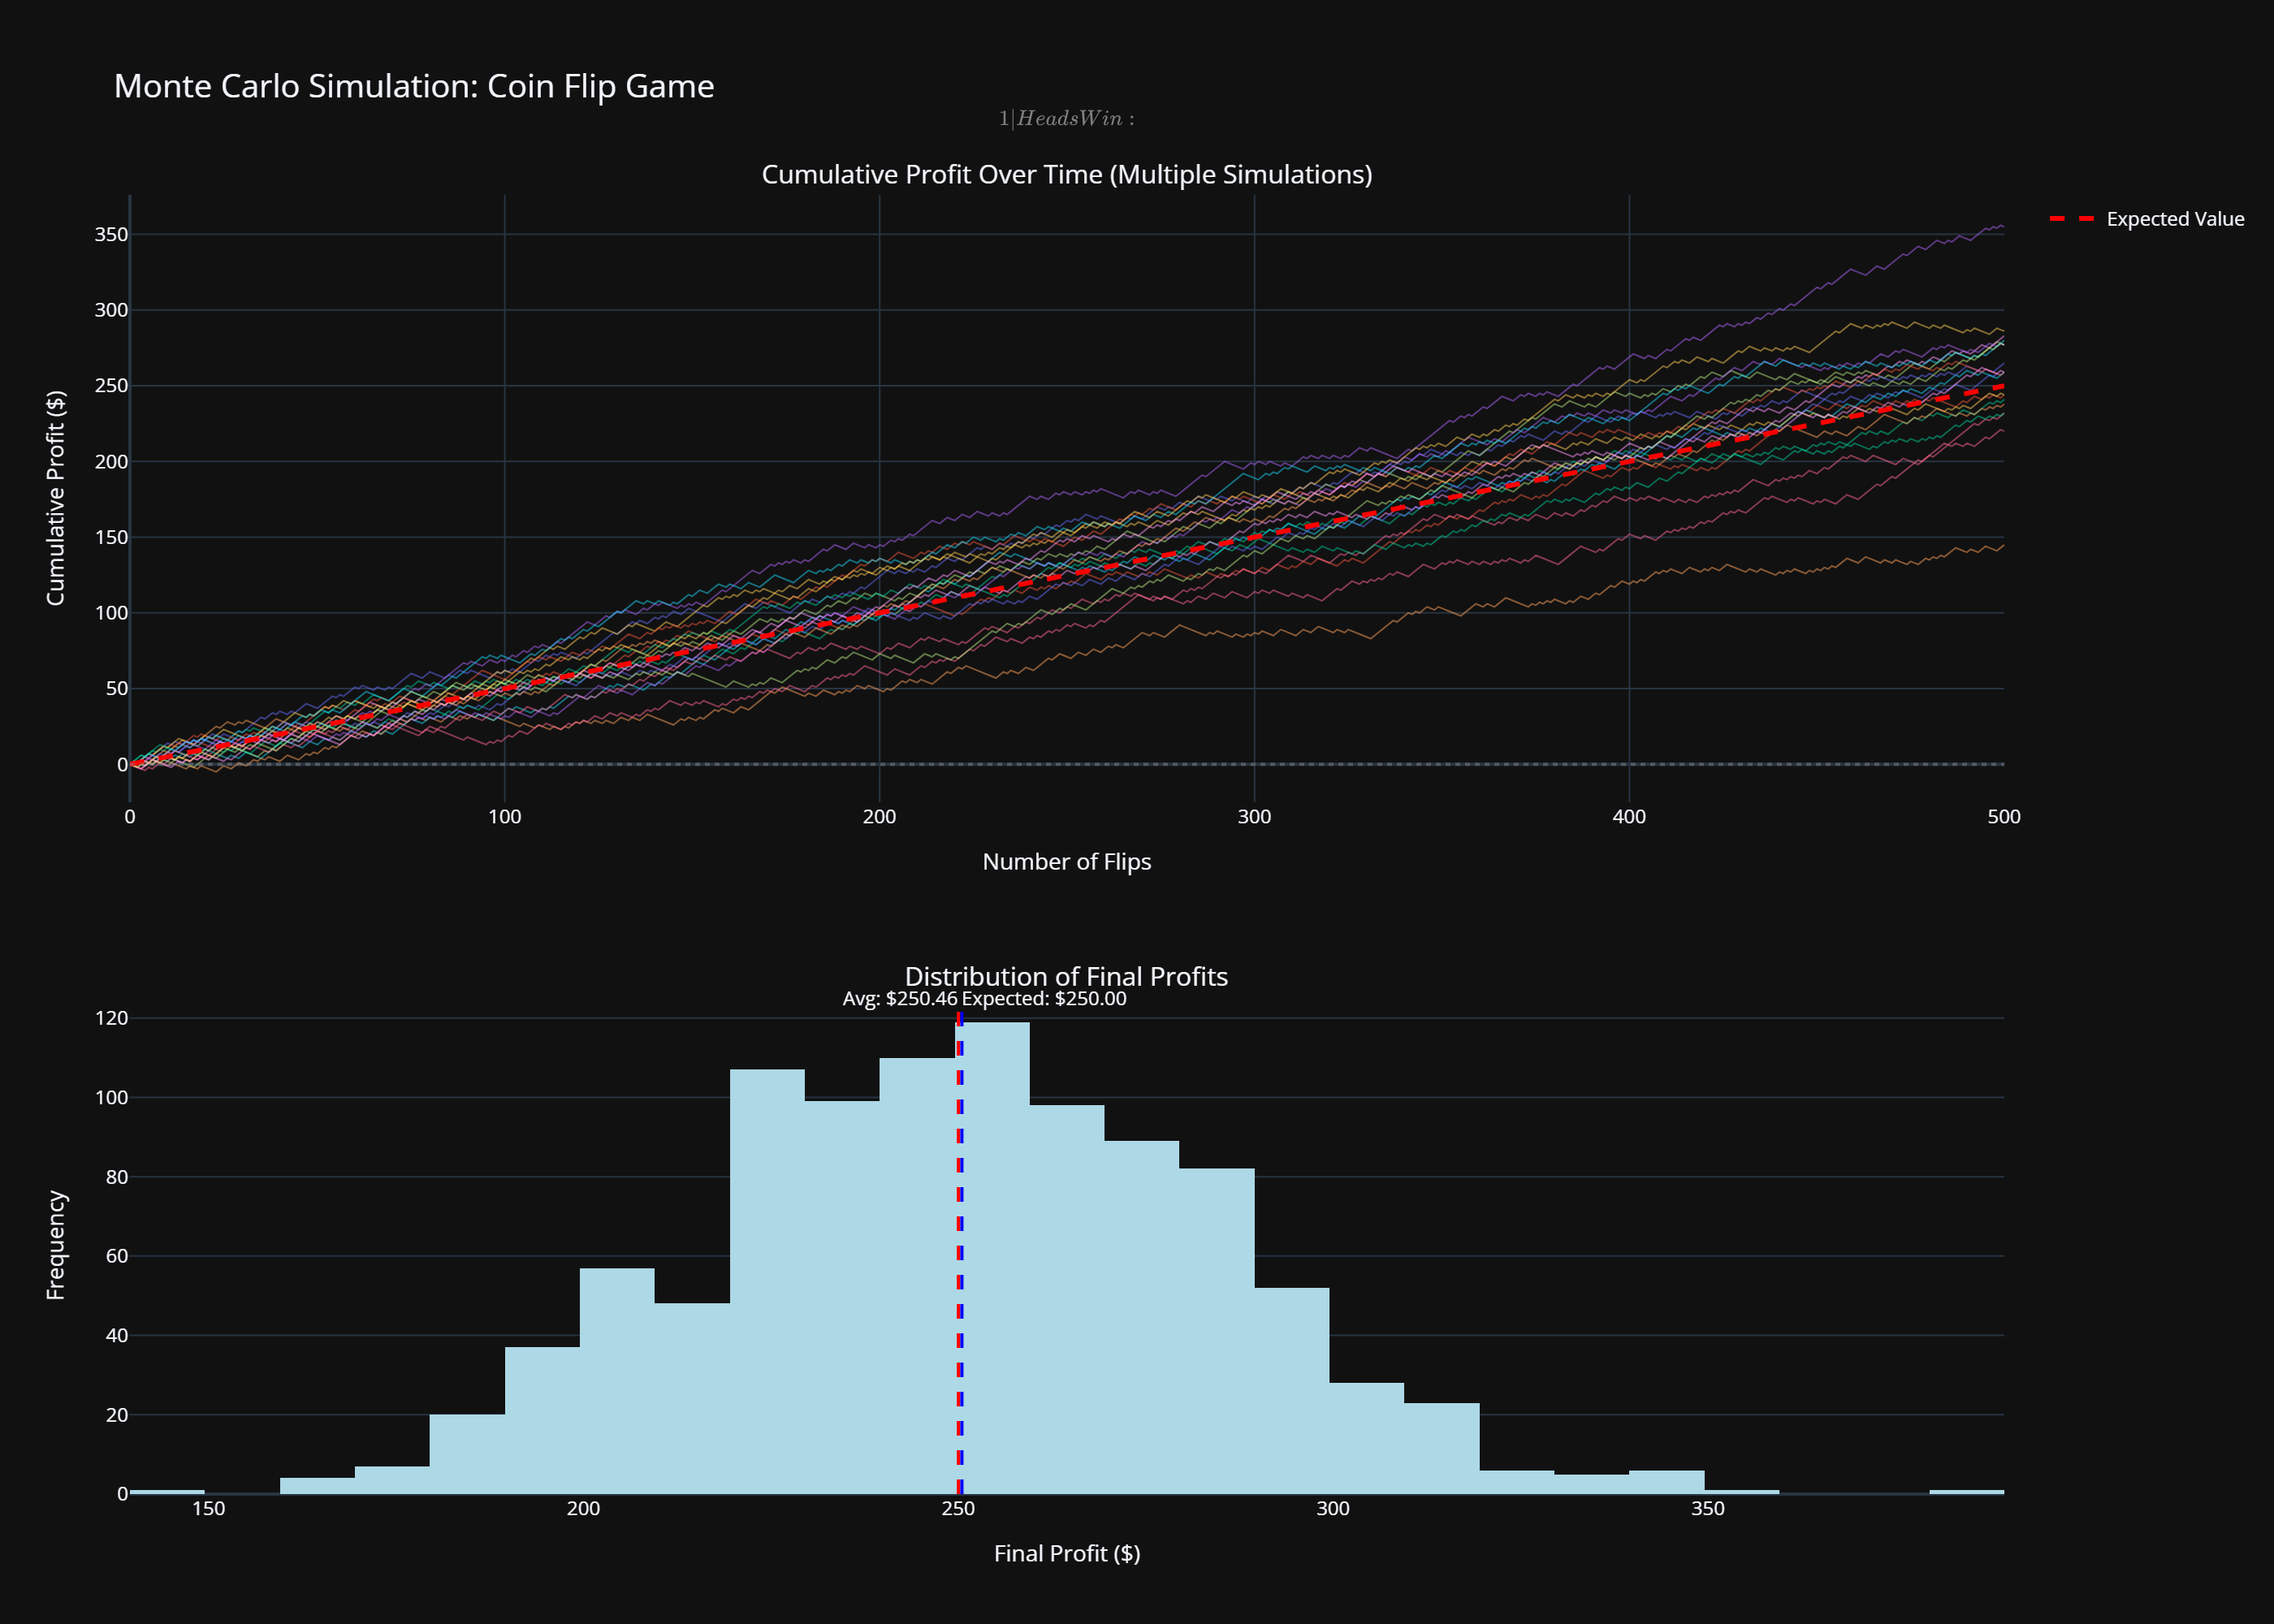
\includegraphics[width=0.8\textwidth]{+ev/500+ev.png}
\caption{Simulation with 500 flips (+EV).}
\end{figure}

\begin{figure}[h!]
\centering
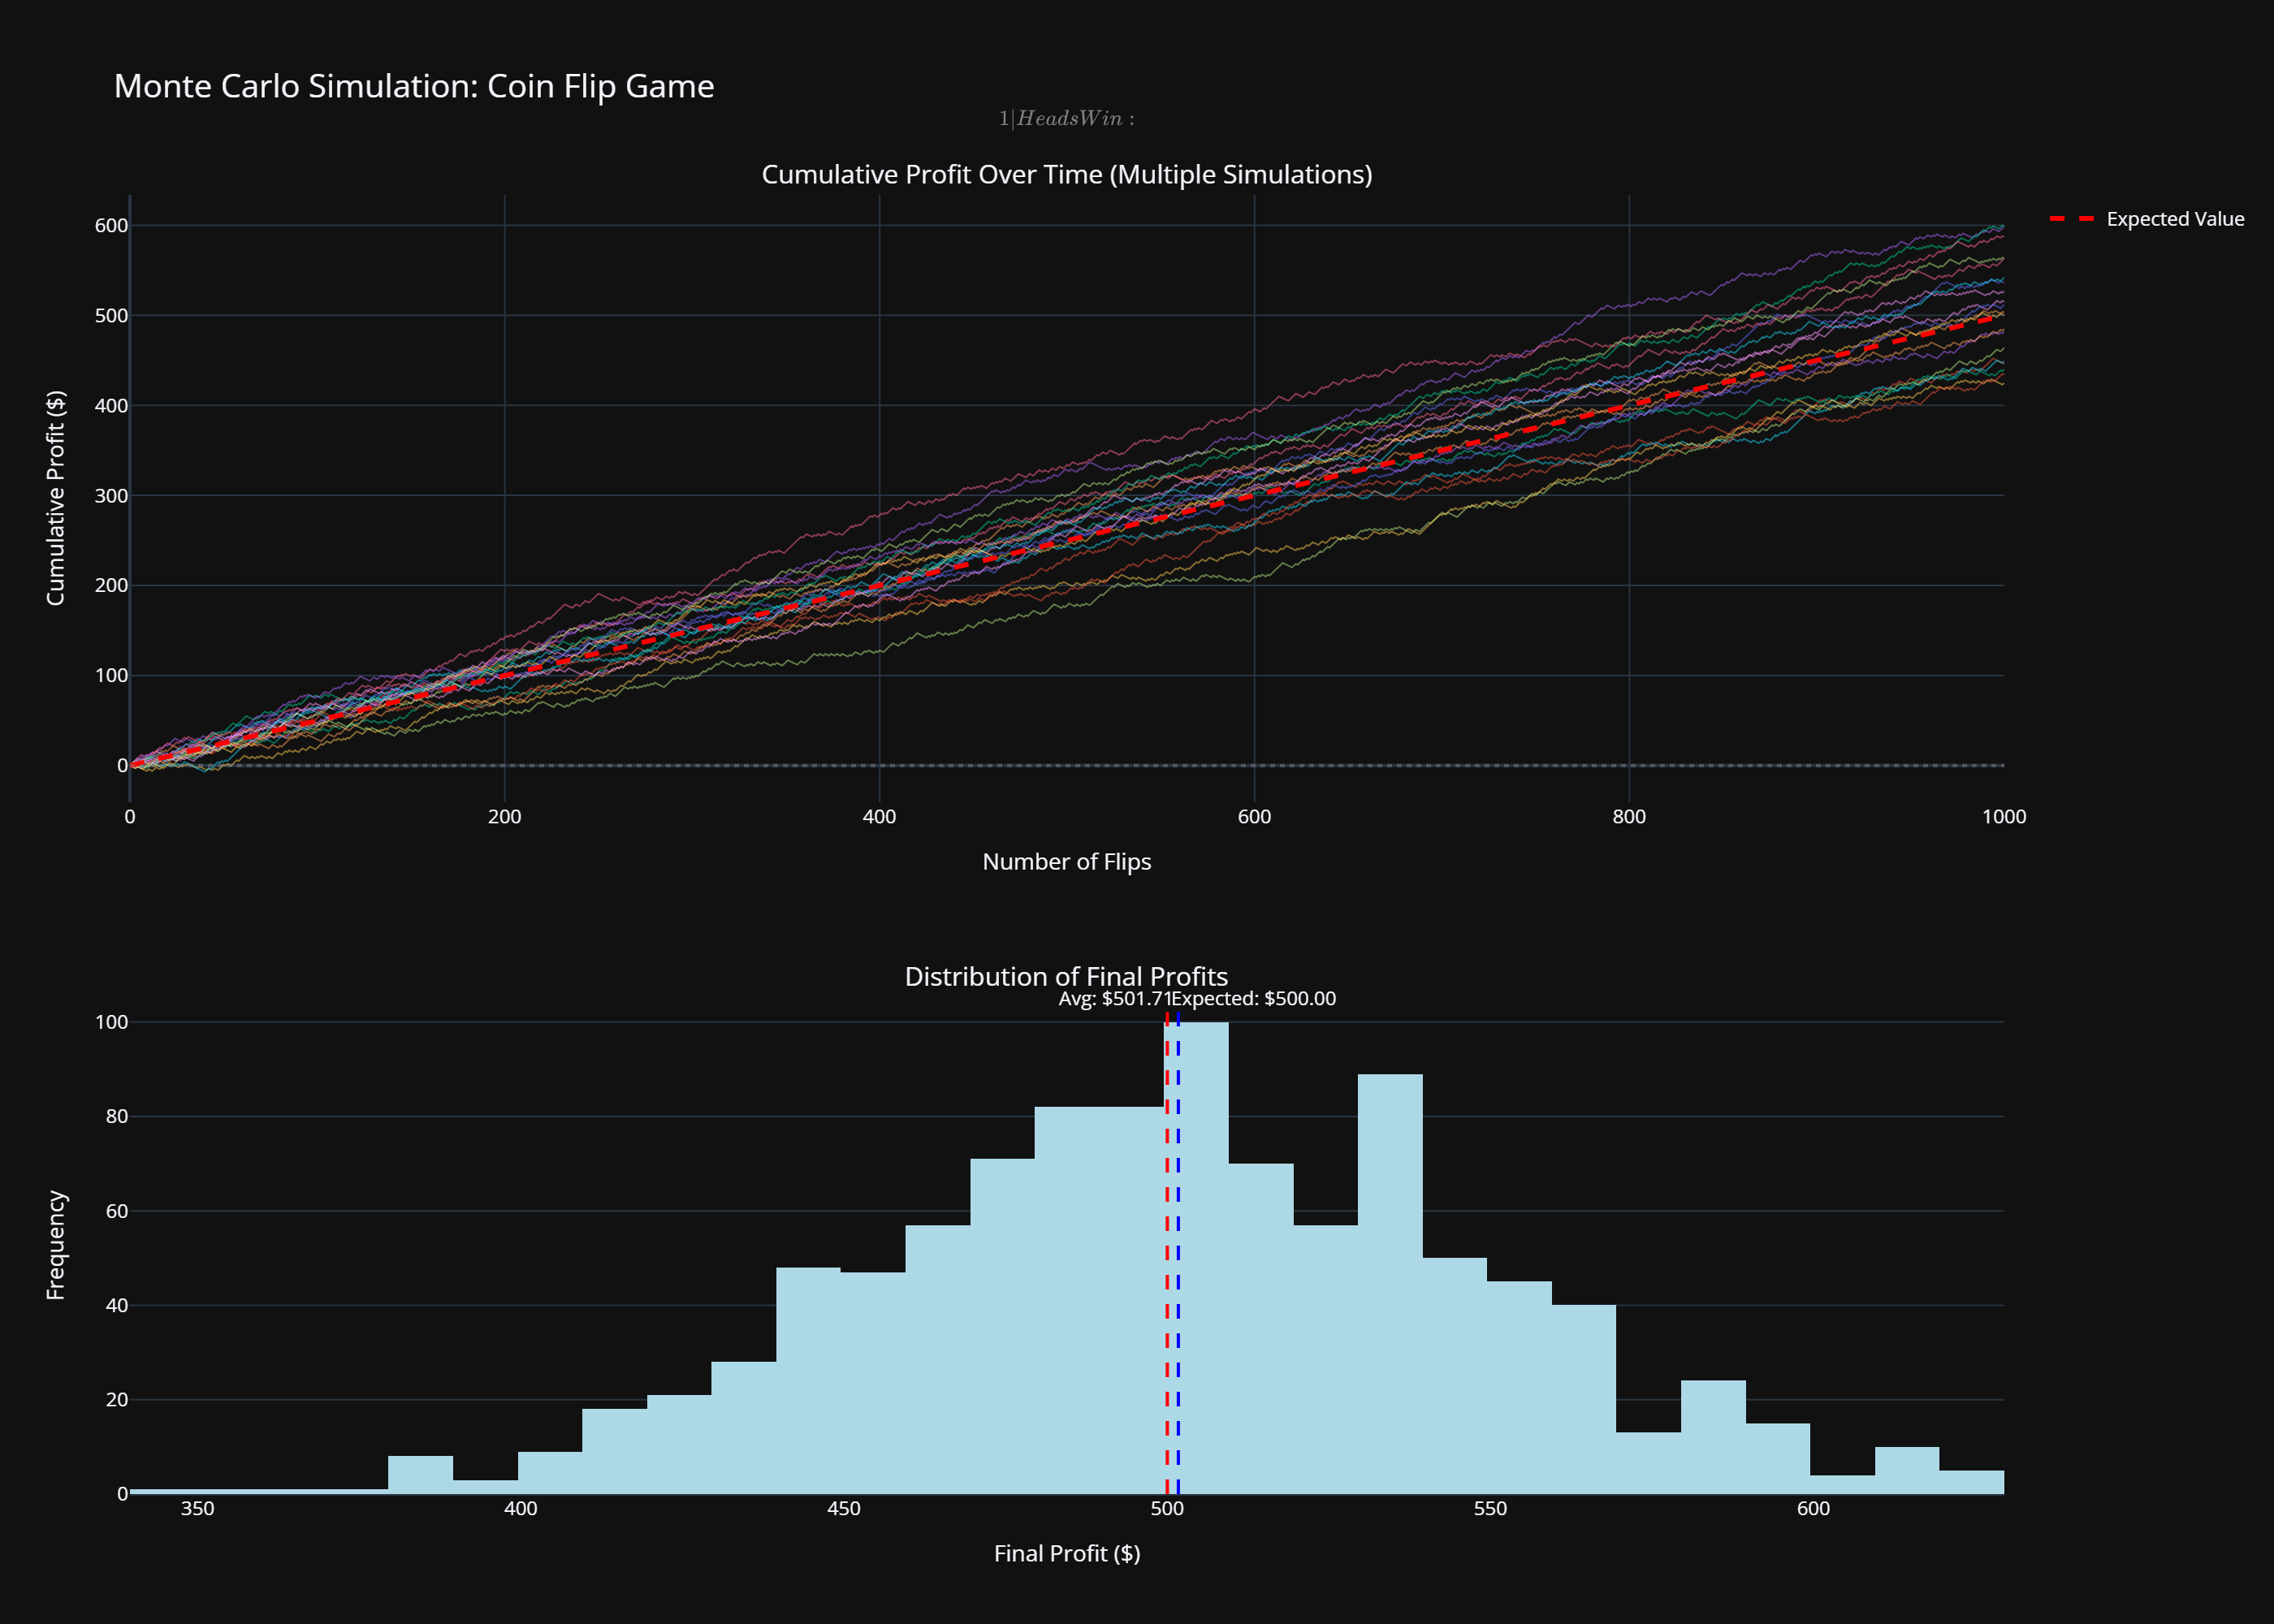
\includegraphics[width=0.8\textwidth]{+ev/1000+ev.png}
\caption{Simulation with 1,000 flips (+EV). Individual paths now closely follow the EV.}
\end{figure}
\clearpage

\subsubsection{10,000 Flips}
With a vast number of flips, the outcome is almost a certainty. The variance of the average profit per flip is now incredibly small, as $\frac{\sigma^2}{n}\to 0$. All simulation paths adhere tightly to the theoretical expectation. The randomness has been effectively "averaged out," leaving only the underlying statistical edge.

\begin{figure}[h!]
\centering
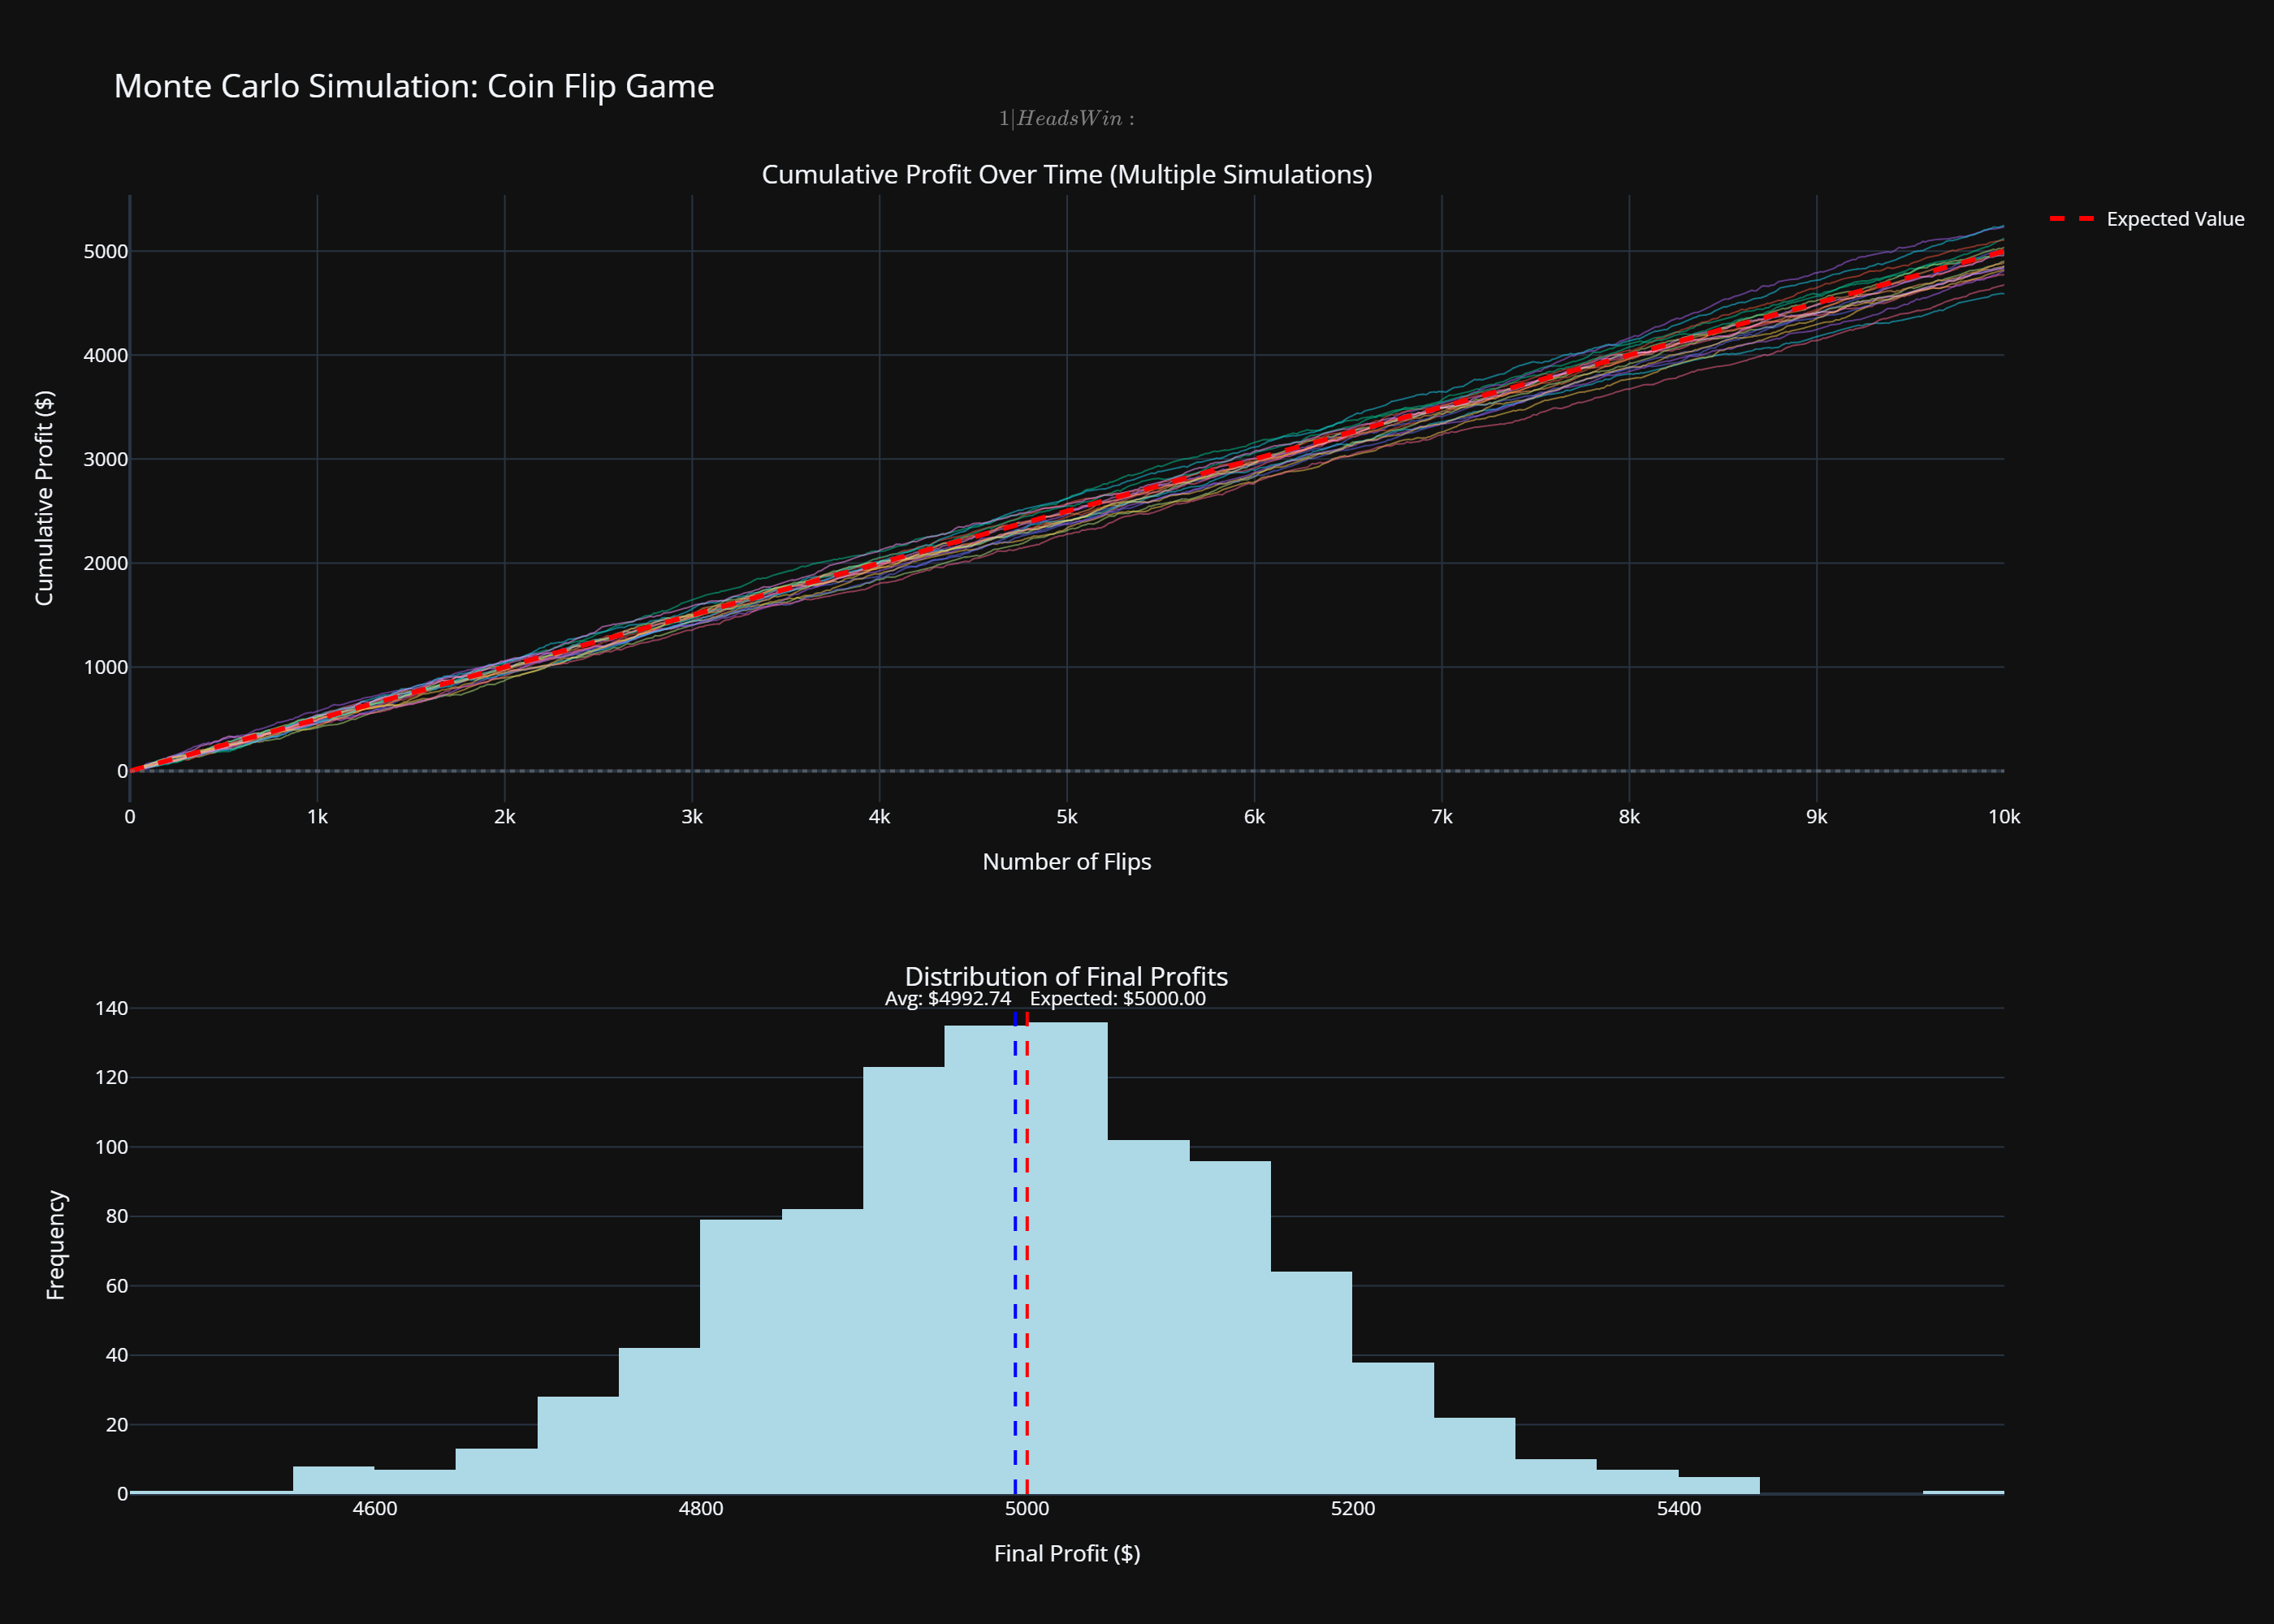
\includegraphics[width=0.8\textwidth]{+ev/10k+ev.png}
\caption{Simulation with 10,000 flips (+EV). Convergence to EV is nearly perfect.}
\end{figure}

% --- SECTION 3: NEGATIVE EV SIMULATION ---
\section{Case Study 2: The Negative EV Game}
This game mirrors those found in casinos, where the rules create a long-term disadvantage for the player.

\subsection{Game Rules and Calculation}
\begin{itemize}
    \item \textbf{Cost to Play:} \$2.00
    \item \textbf{Heads Payout:} \$3.00 (Net profit: \$1.00)
    \item \textbf{Tails Payout:} \$0.00 (Net loss: \$2.00)
\end{itemize}
The Expected Value per flip is:
\[
EV = (0.5 \times \$1.00) + (0.5 \times -\$2.00) = \$0.50 - \$1.00 = \boldsymbol{-\$0.50}
\]
On average, a player is guaranteed to lose 50 cents per flip over the long run.

\subsection{Simulation Results}
The behavior is a mirror image of the positive EV case. Initial luck may lead to profits, but the mathematical disadvantage inevitably pulls the cumulative results downward as the number of flips increases.

\begin{figure}[h!]
\centering
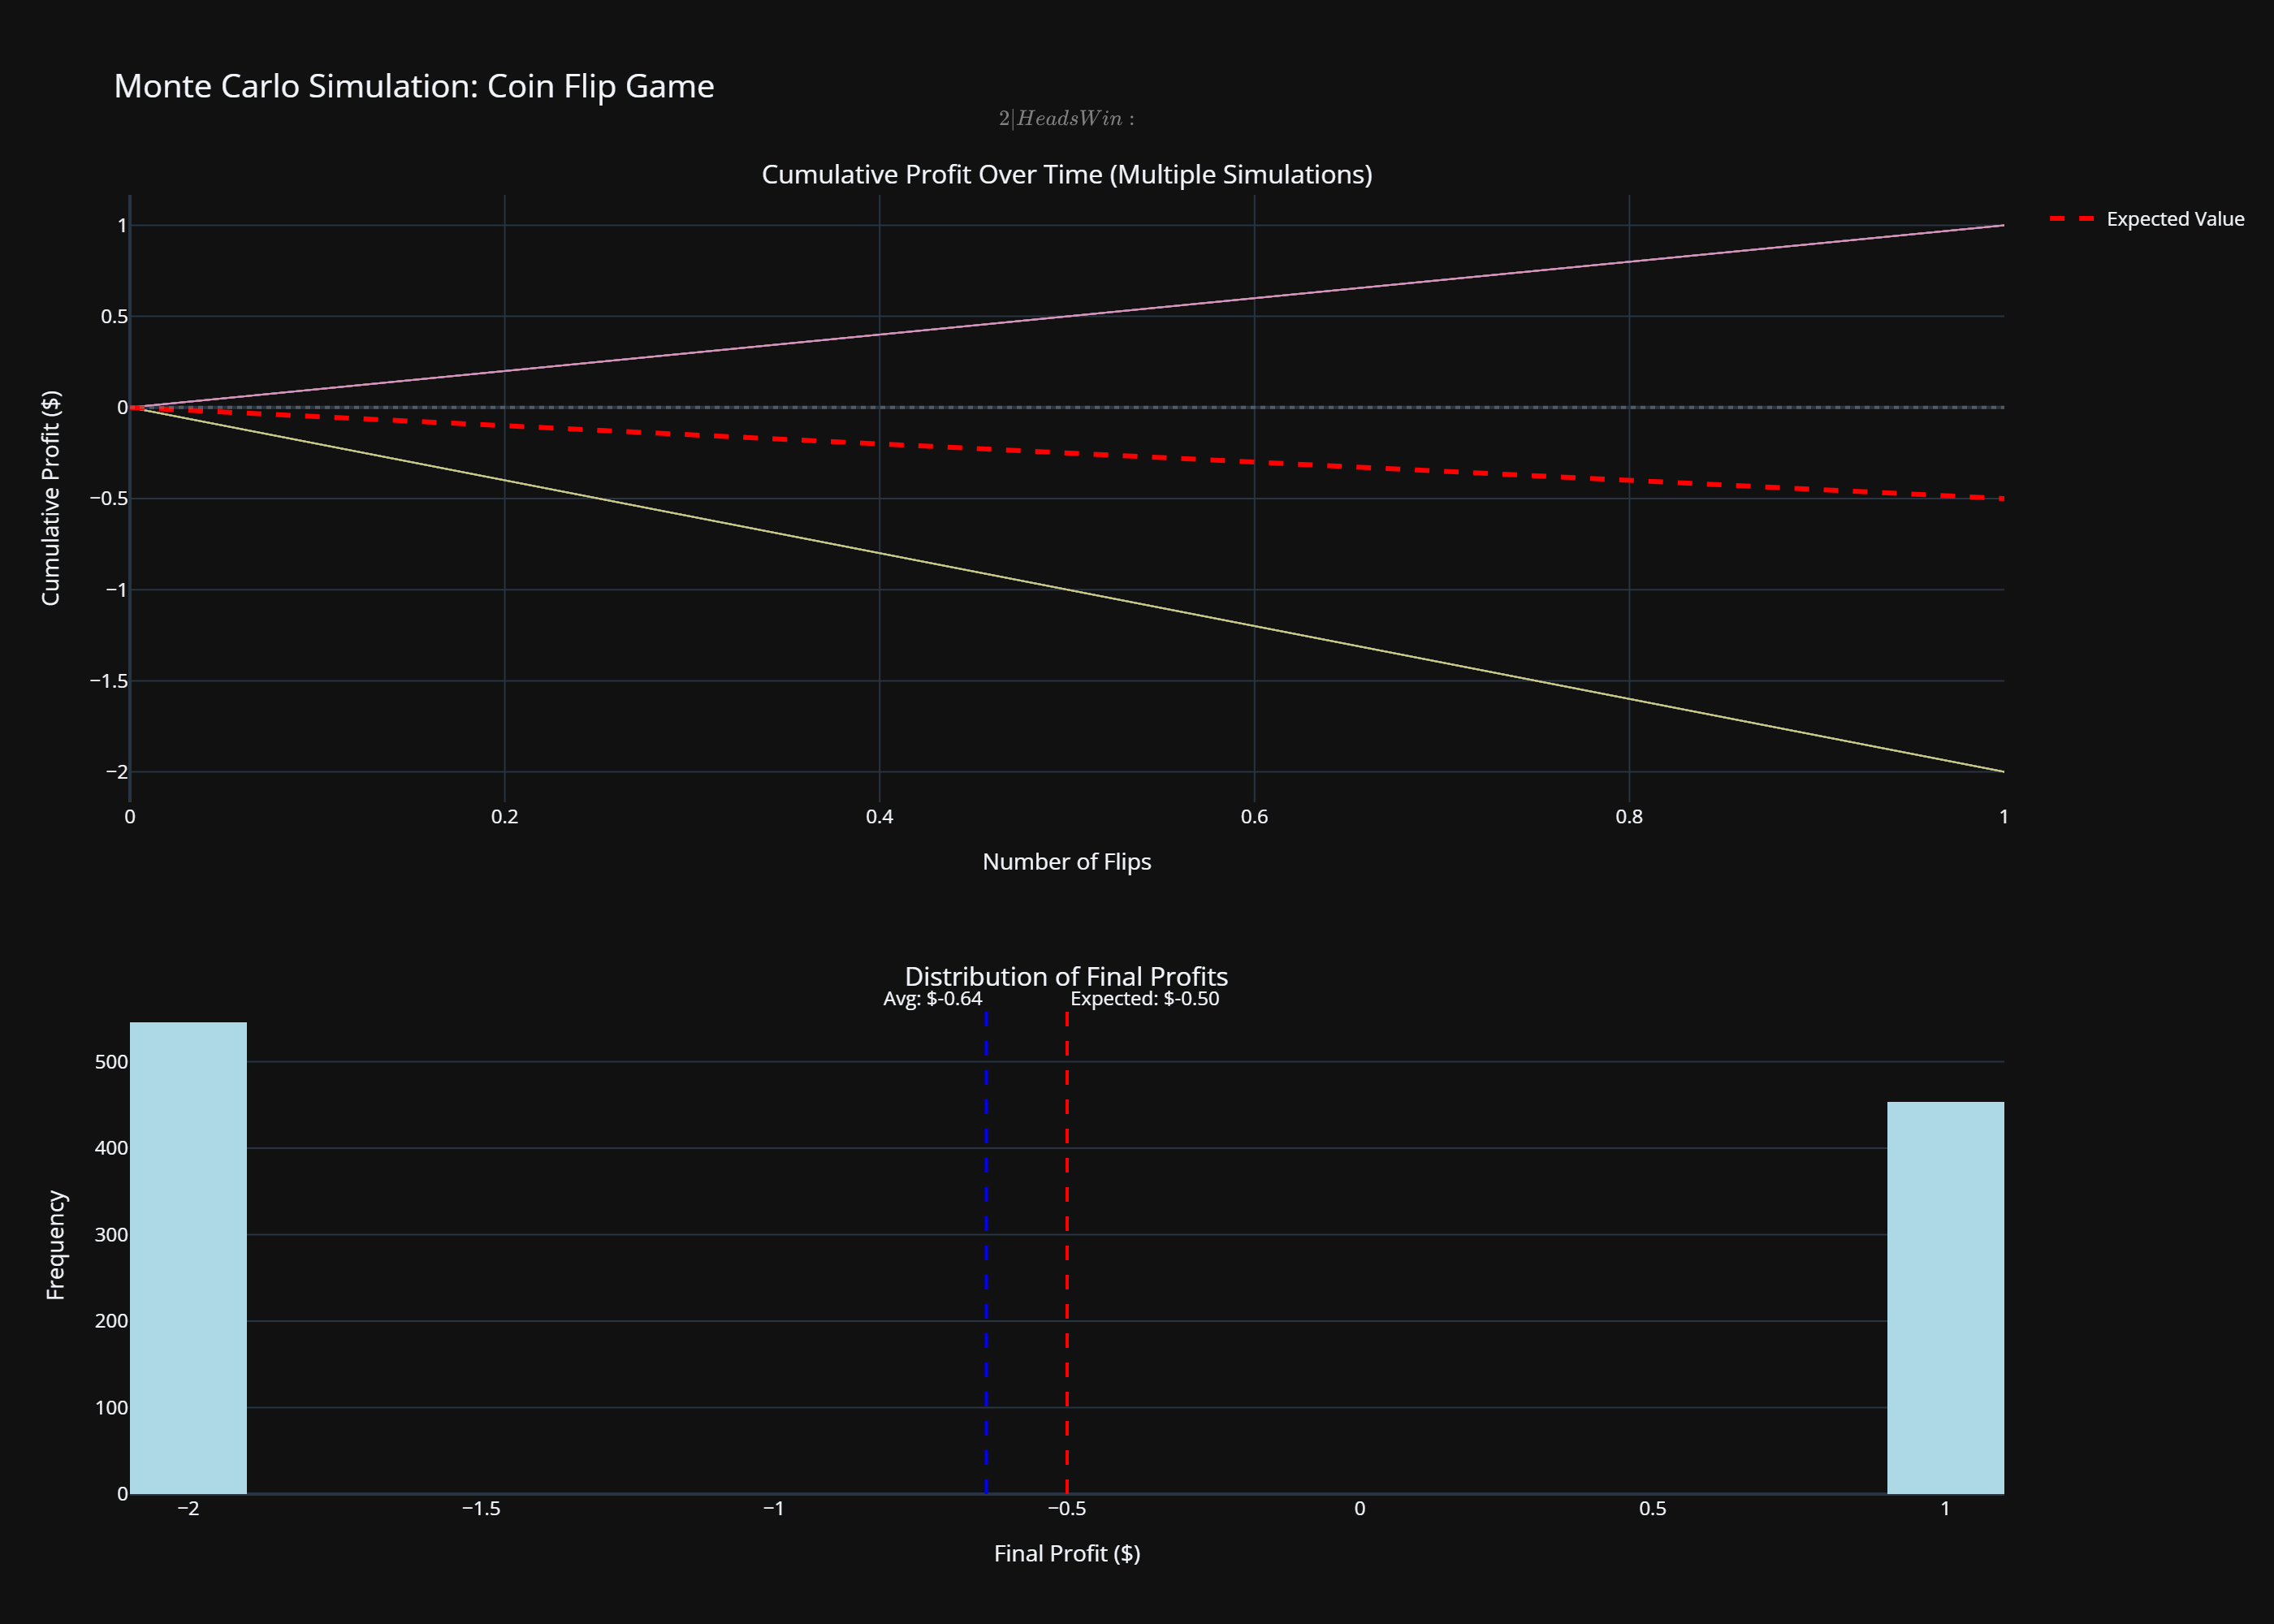
\includegraphics[width=0.8\textwidth]{-ev/1-ev.png}
\caption{Simulation with 1 flip (-EV). Outcome is +\$1 or -\$2.}
\end{figure}

\begin{figure}[h!]
\centering
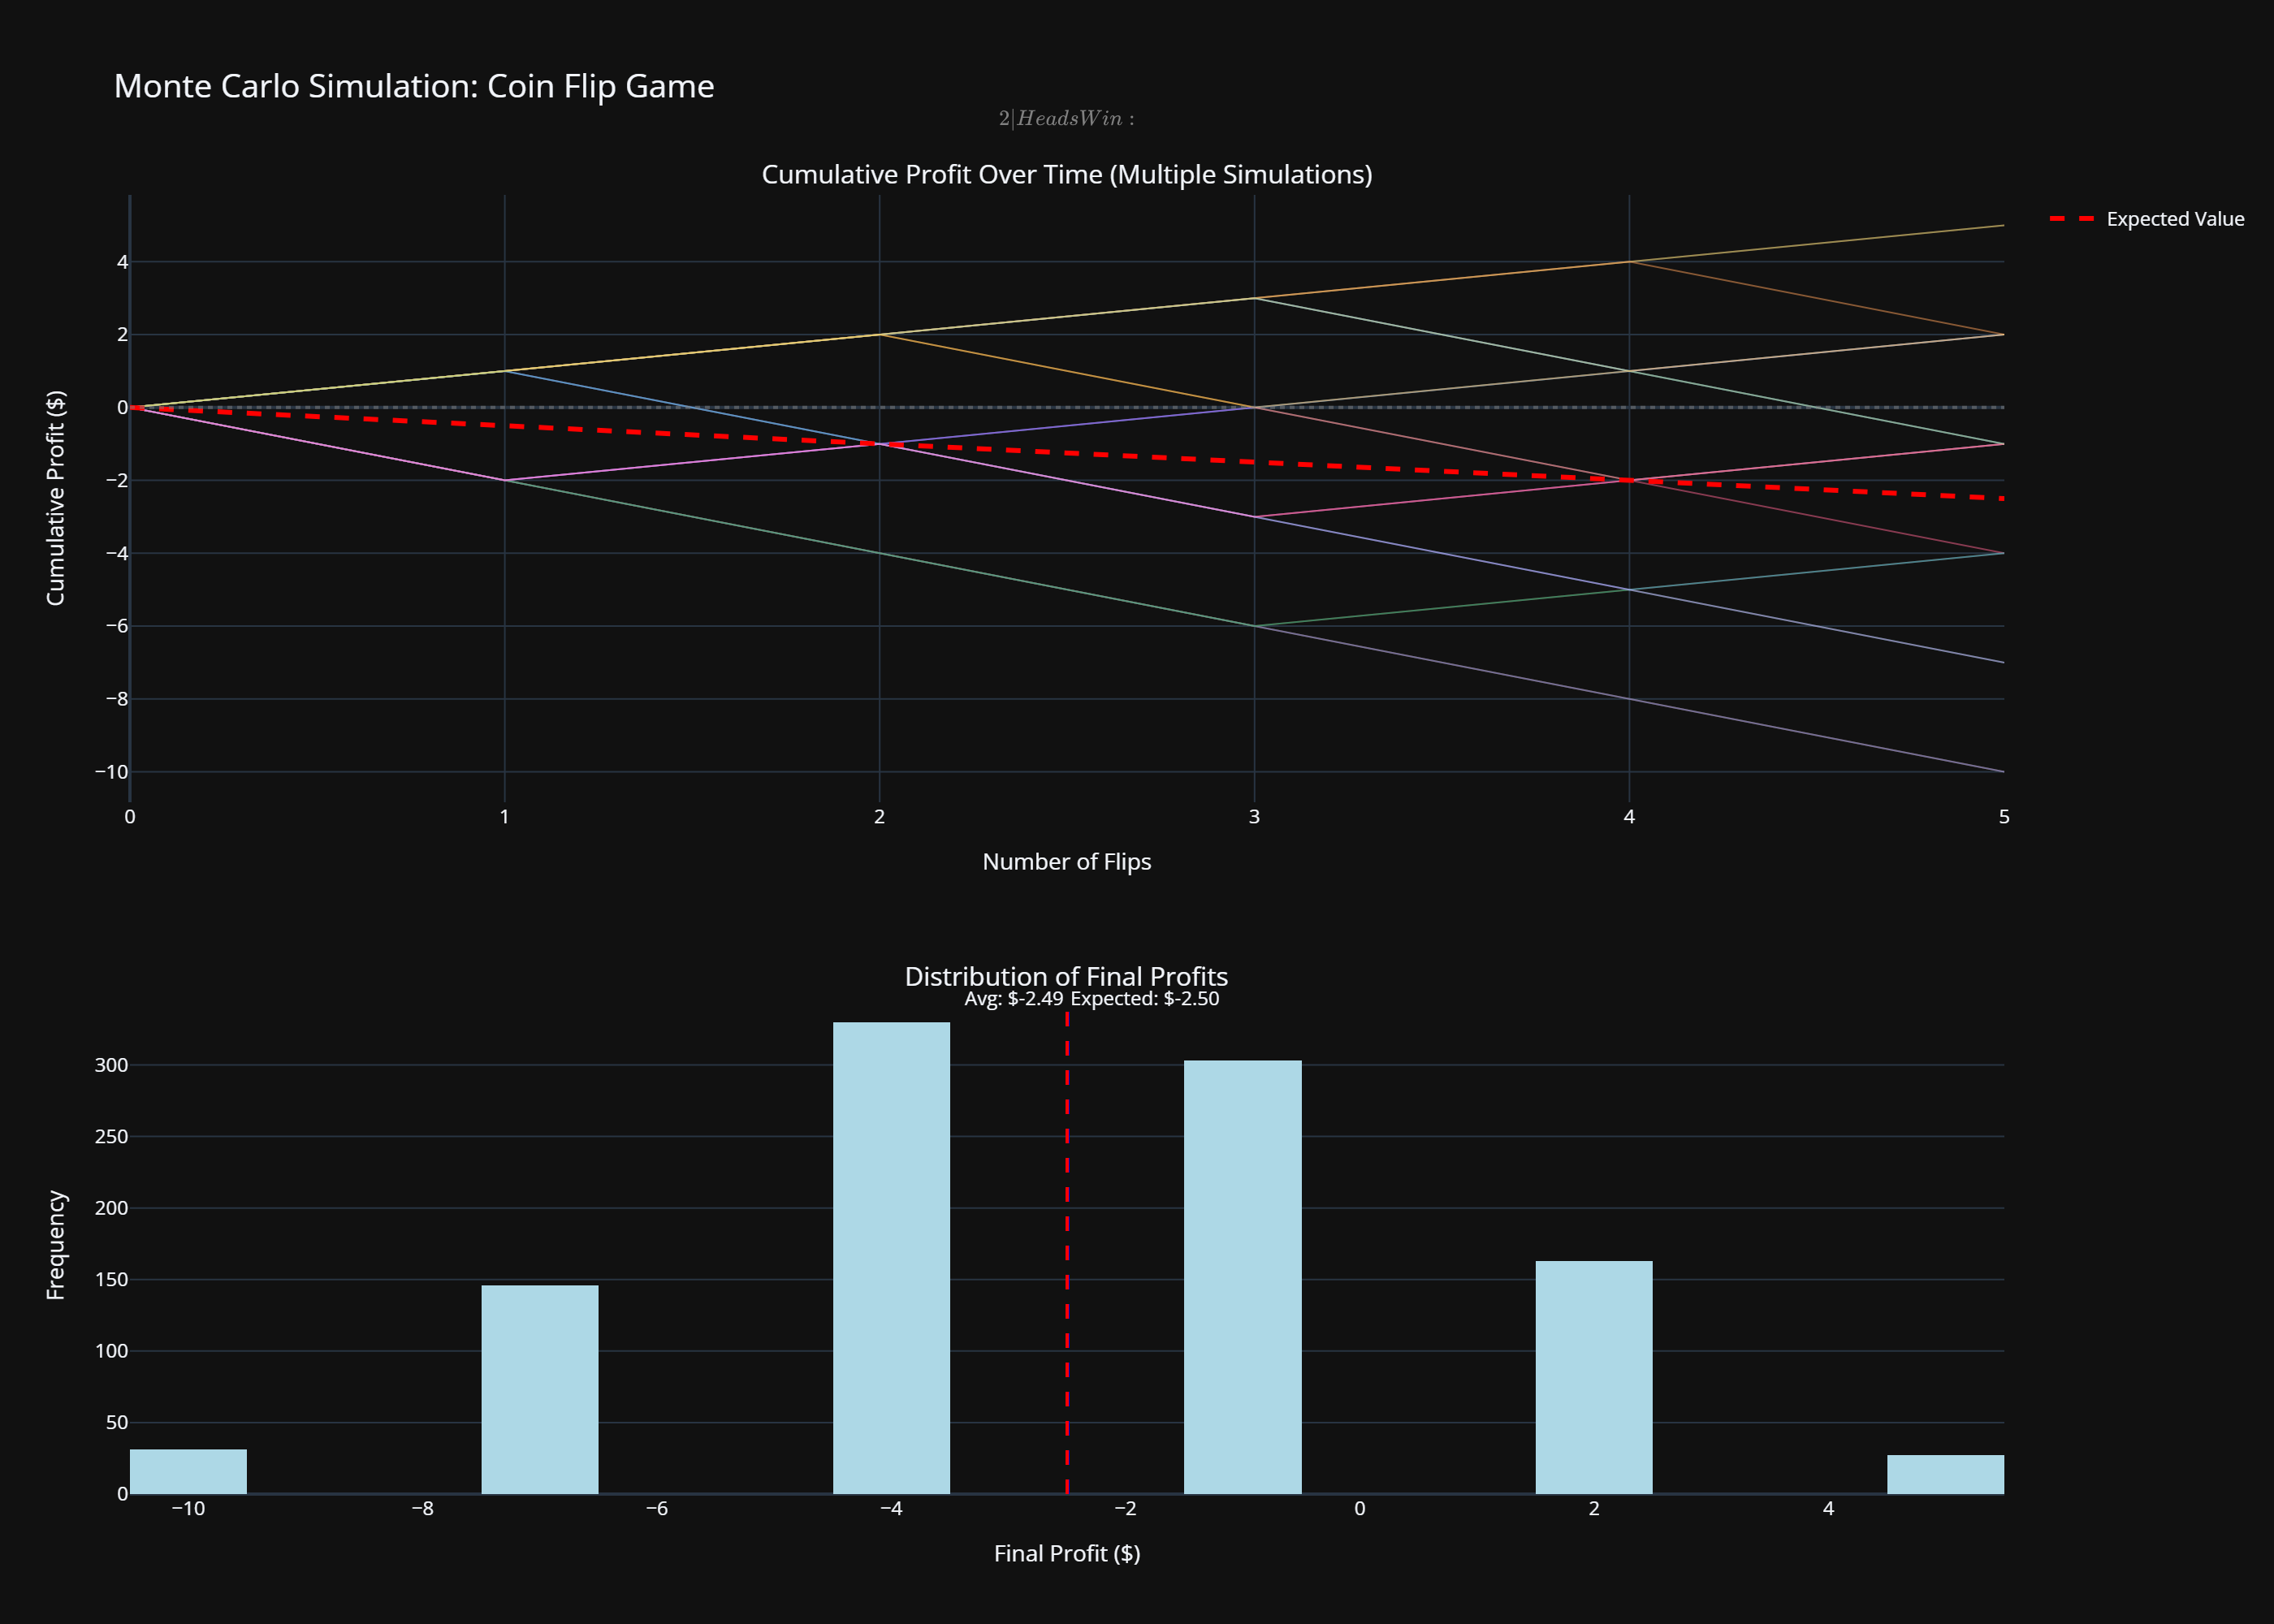
\includegraphics[width=0.8\textwidth]{-ev/5-ev.png}
\caption{Simulation with 5 flips (-EV).}
\end{figure}
\clearpage

\begin{figure}[h!]
\centering
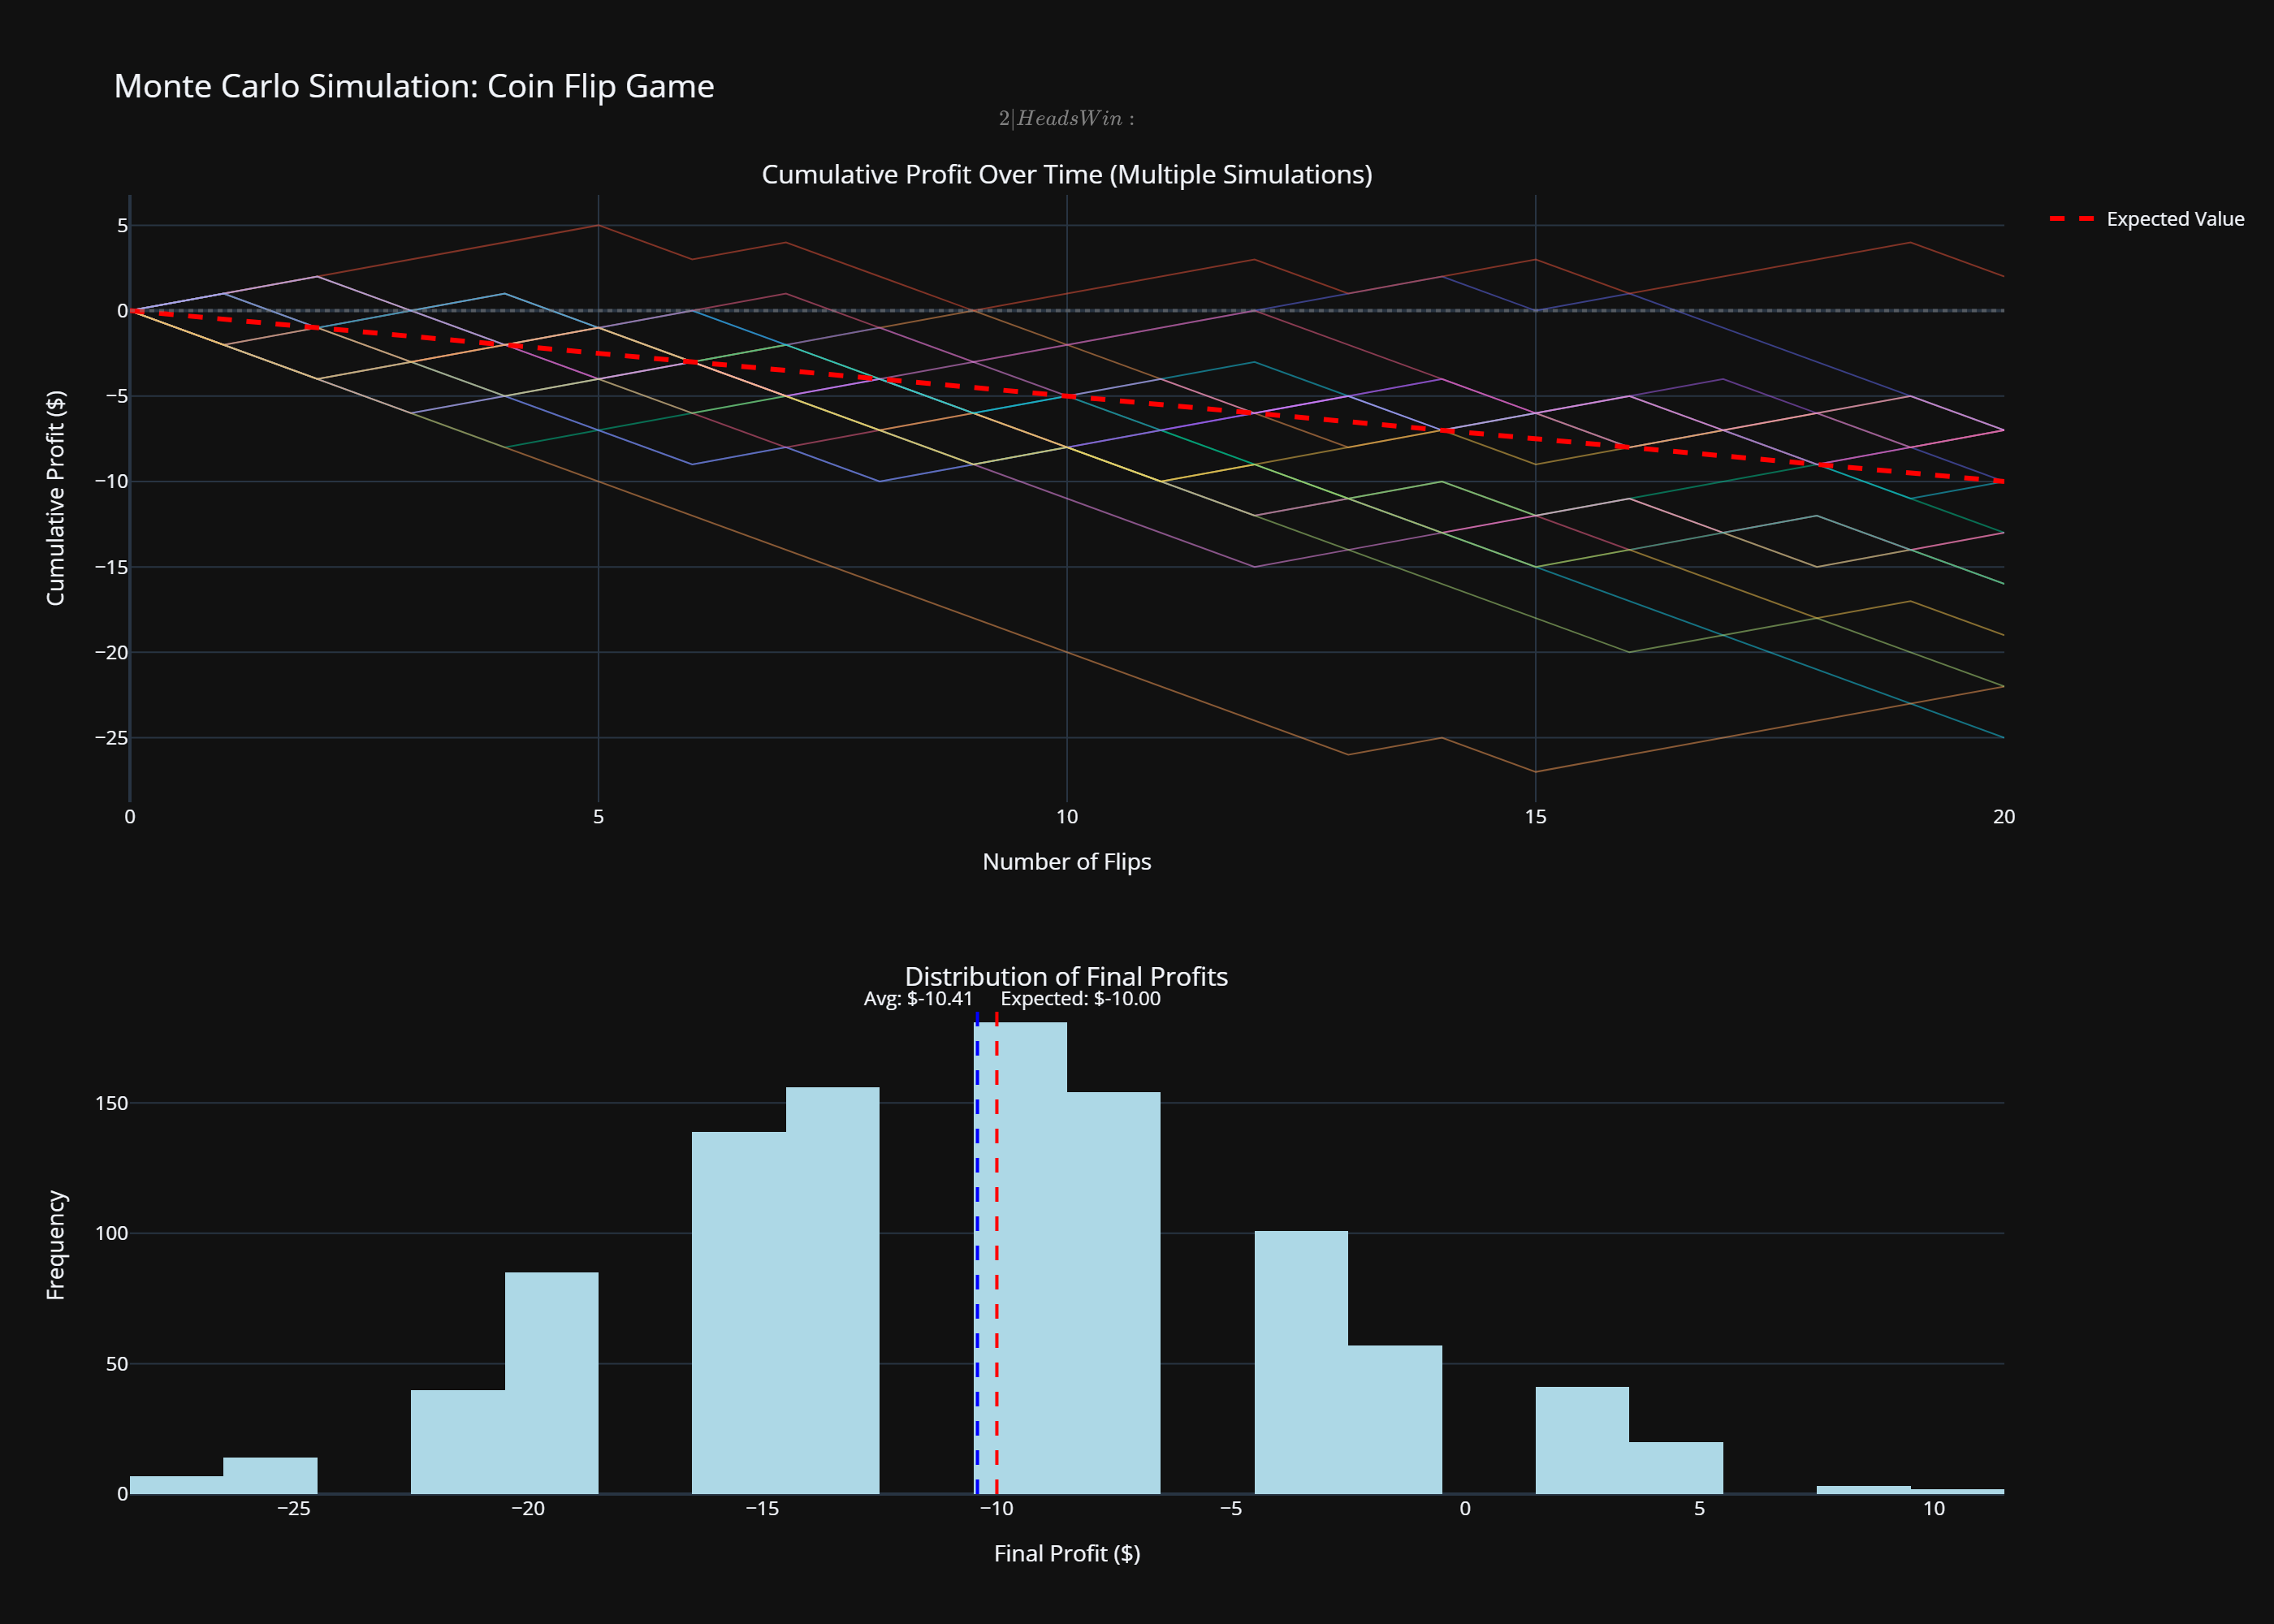
\includegraphics[width=0.8\textwidth]{-ev/20-ev.png}
\caption{Simulation with 20 flips (-EV).}
\end{figure}

\begin{figure}[h!]
\centering
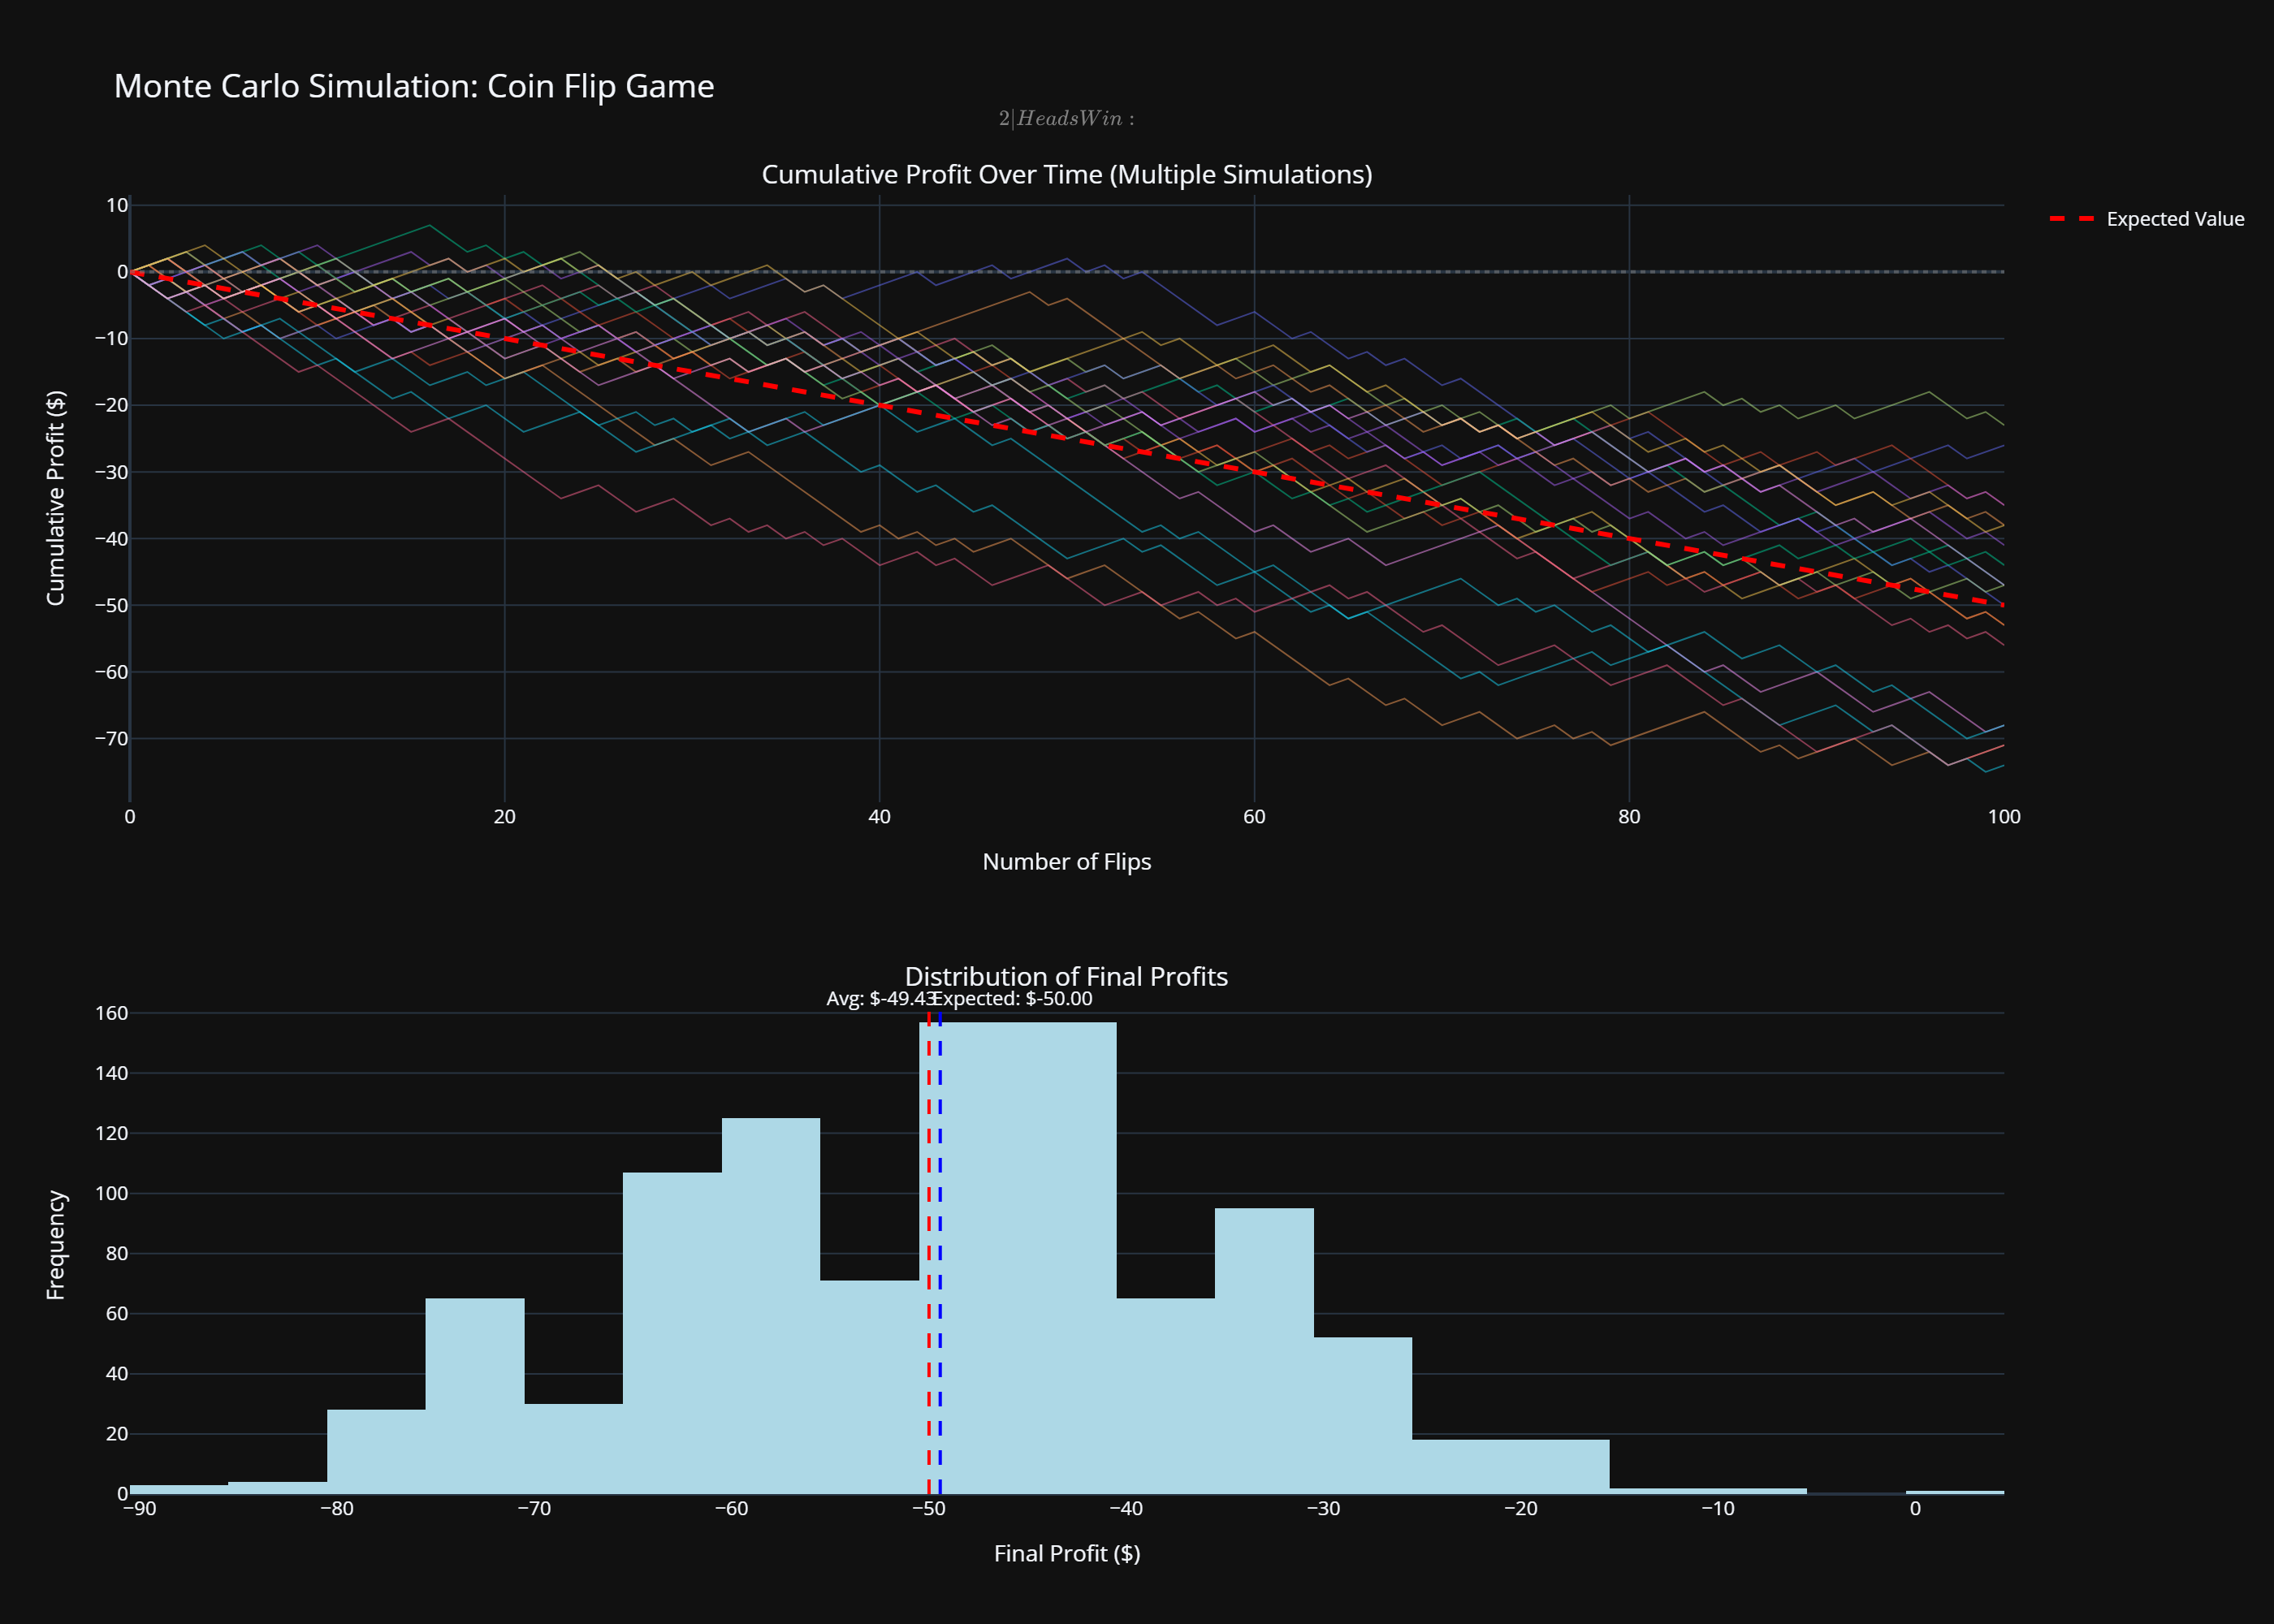
\includegraphics[width=0.8\textwidth]{-ev/100-ev.png}
\caption{Simulation with 100 flips (-EV).}
\end{figure}
\clearpage

\begin{figure}[h!]
\centering
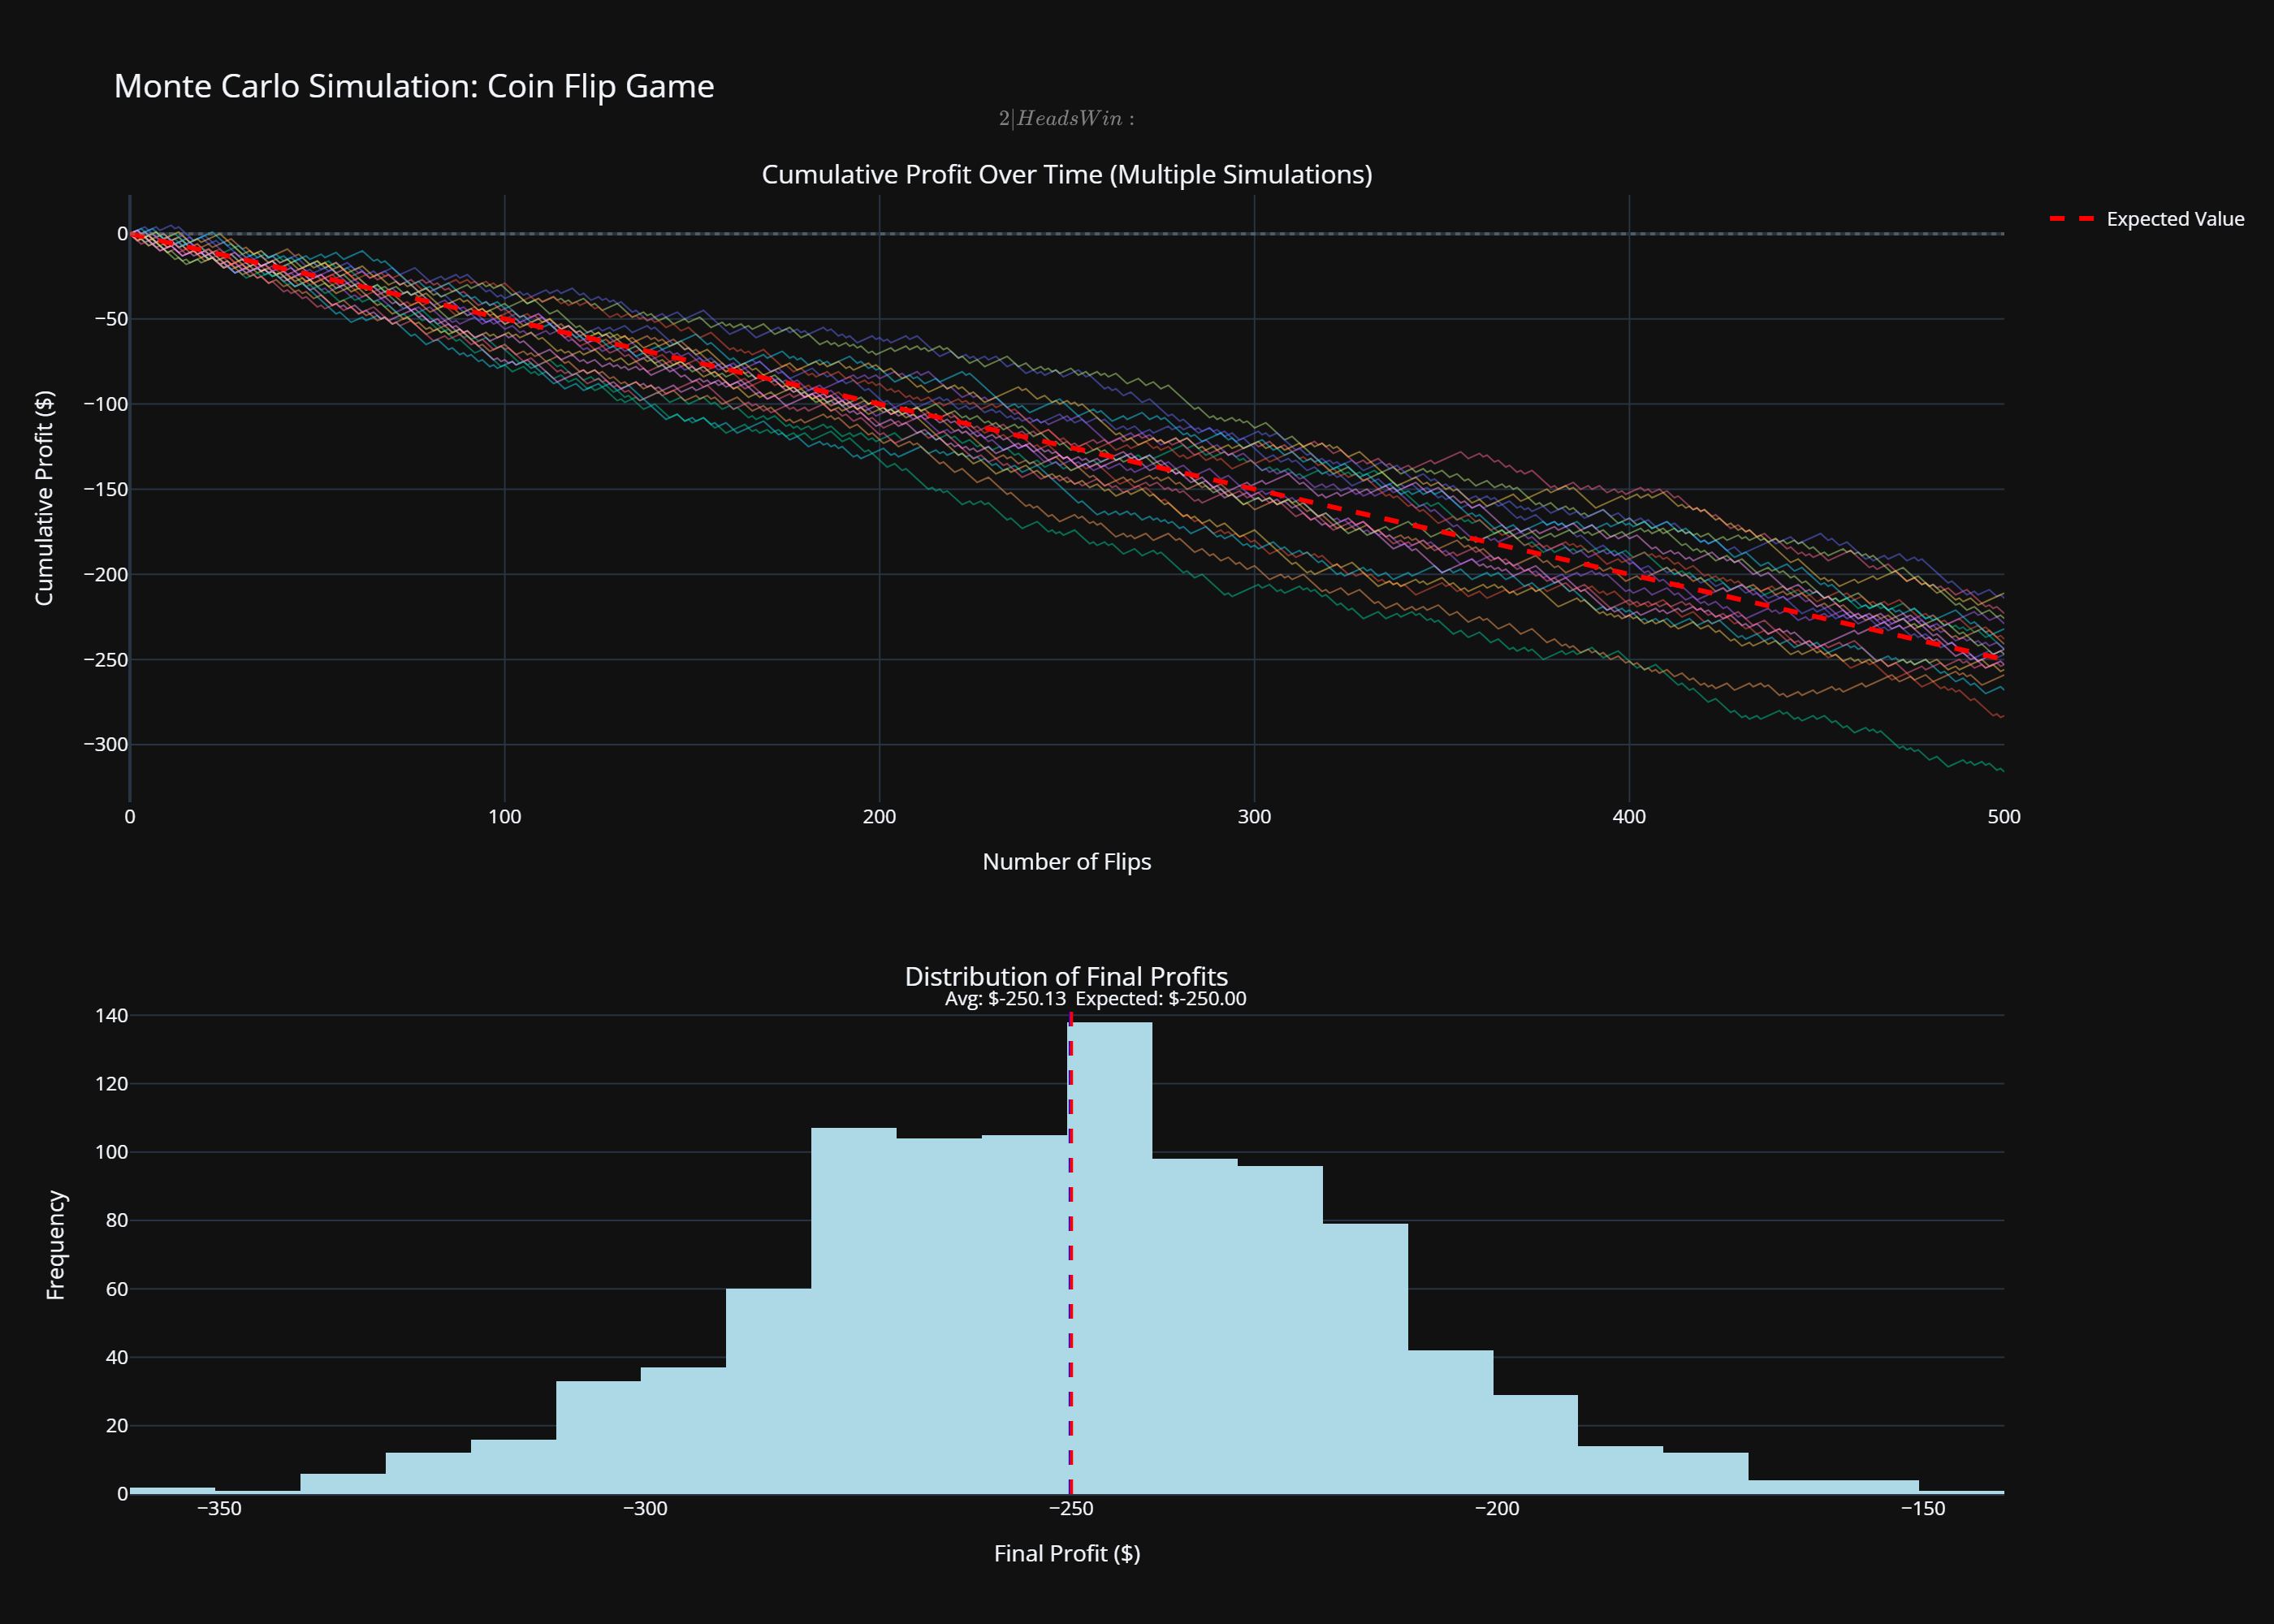
\includegraphics[width=0.8\textwidth]{-ev/500-ev.png}
\caption{Simulation with 500 flips (-EV).}
\end{figure}

\begin{figure}[h!]
\centering
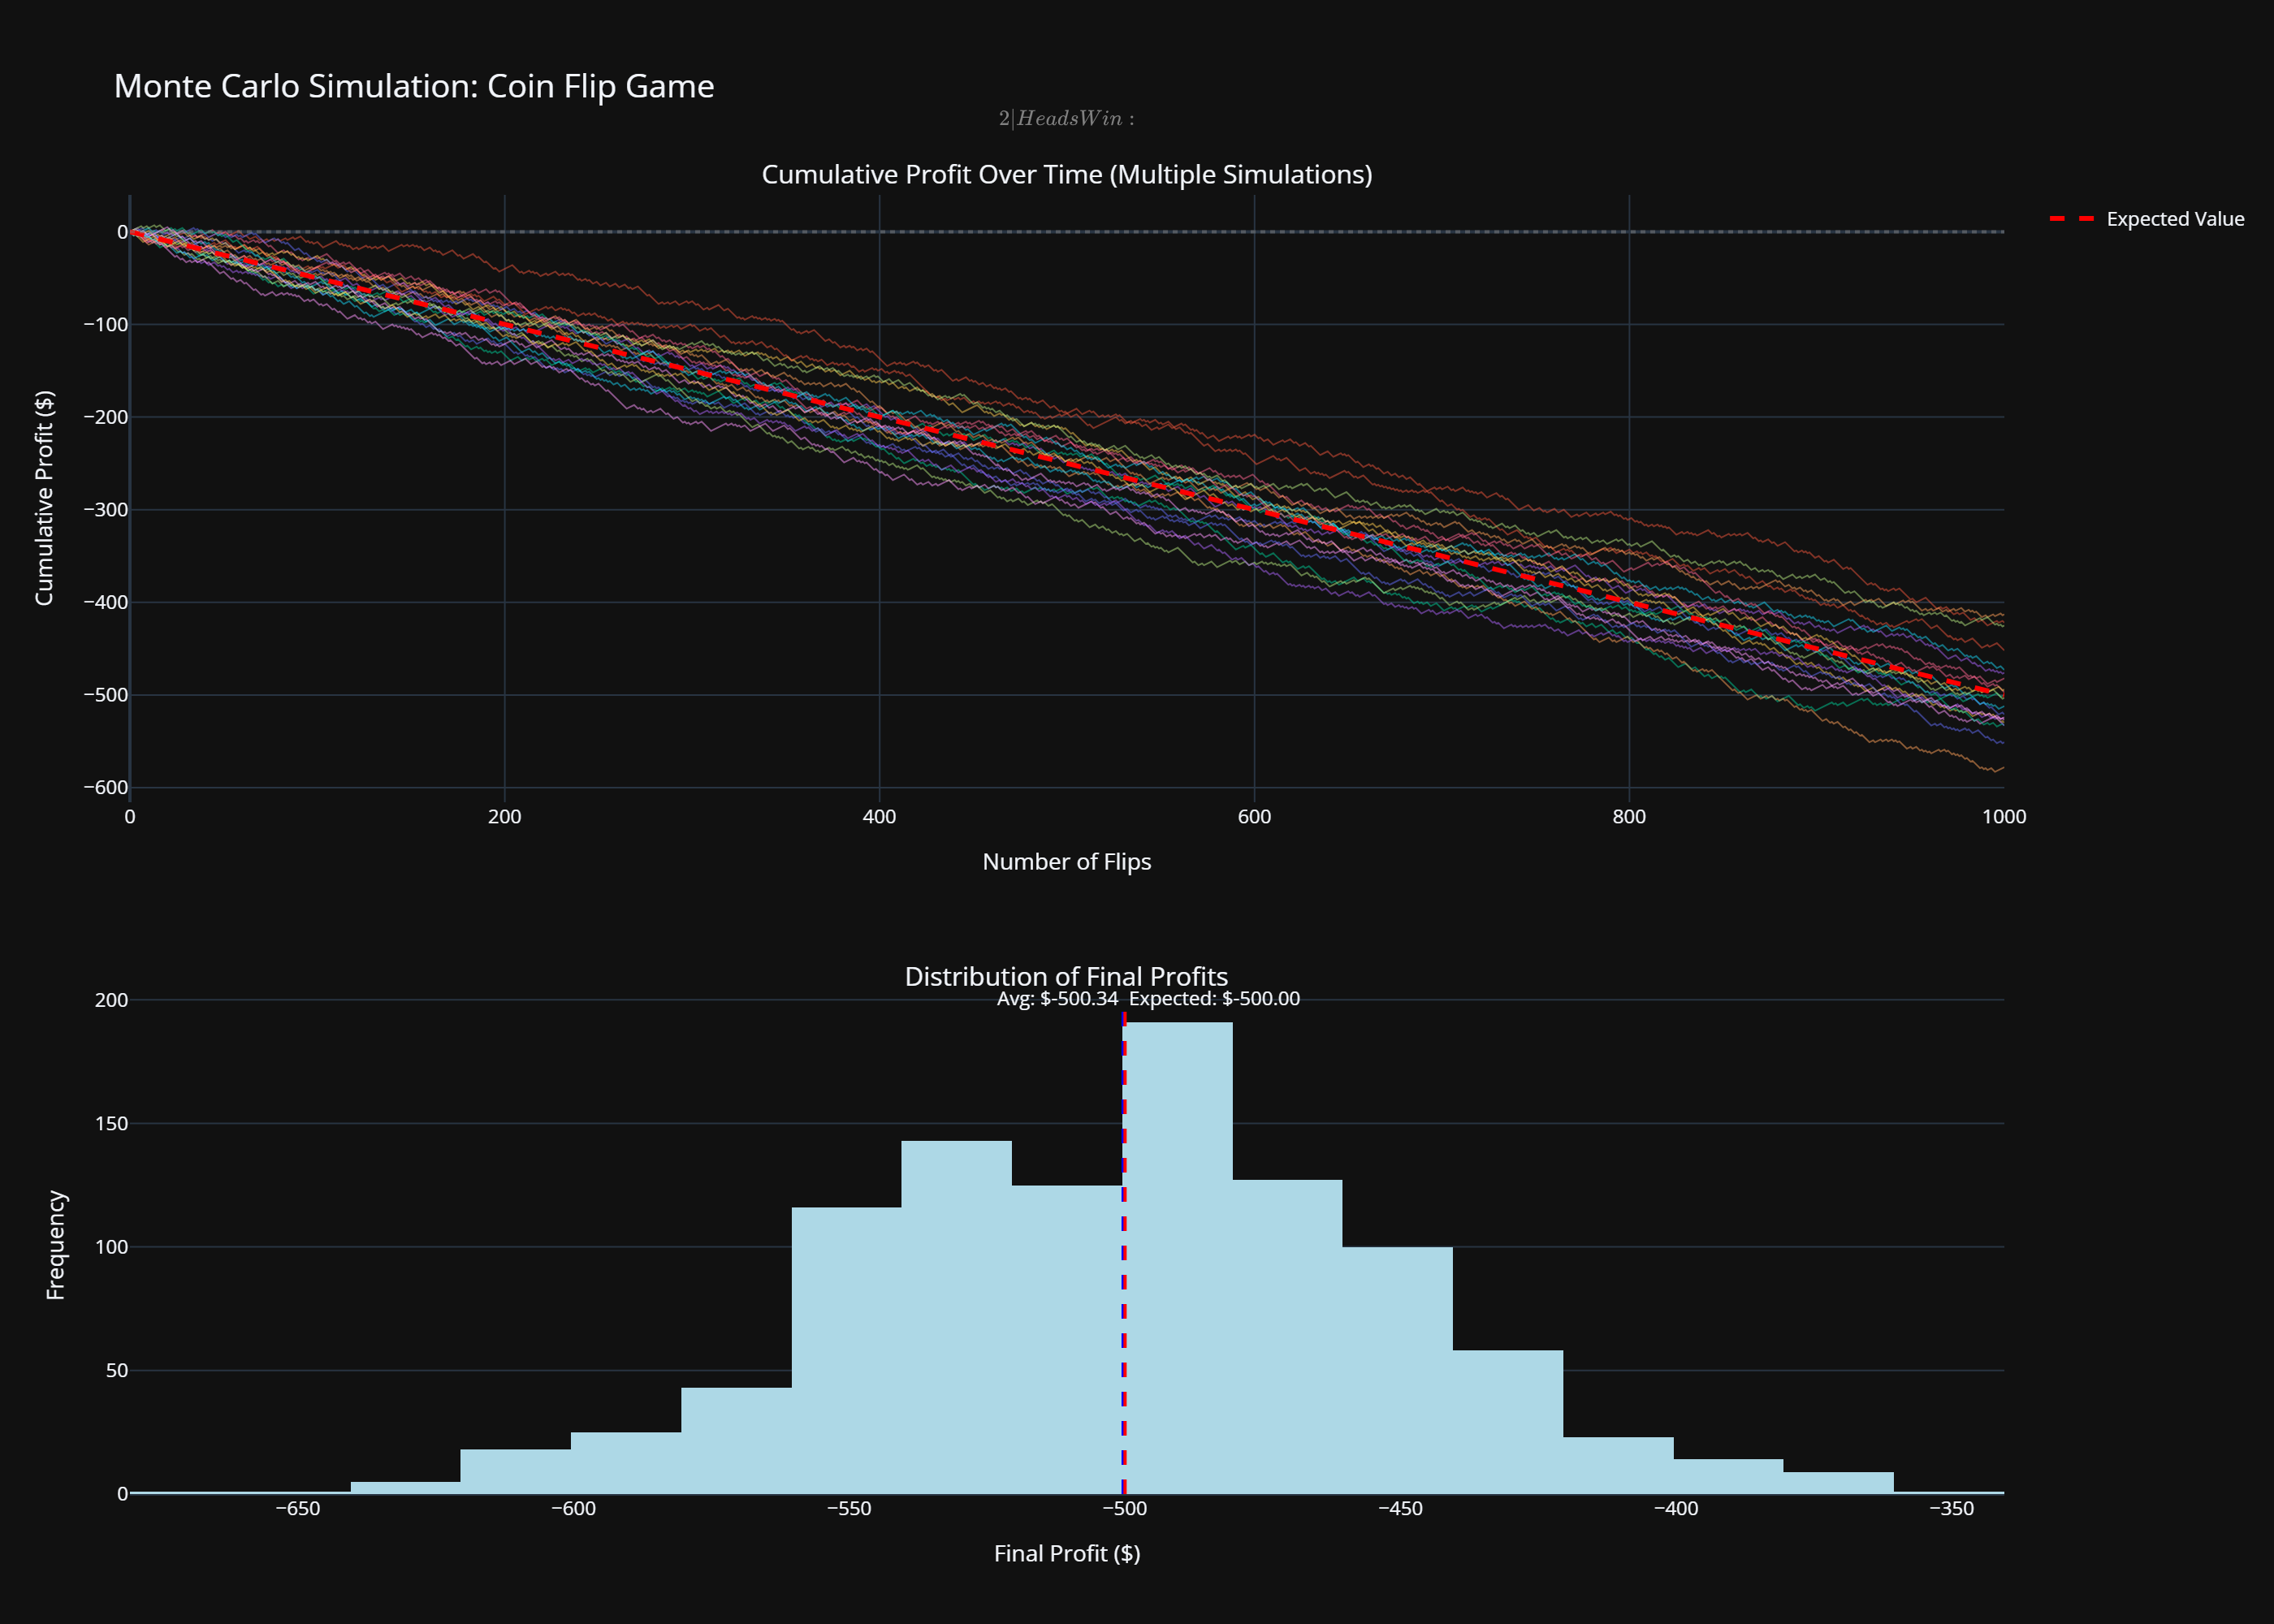
\includegraphics[width=0.8\textwidth]{-ev/1000-ev.png}
\caption{Simulation with 1,000 flips (-EV).}
\end{figure}
\clearpage

\begin{figure}[h!]
\centering
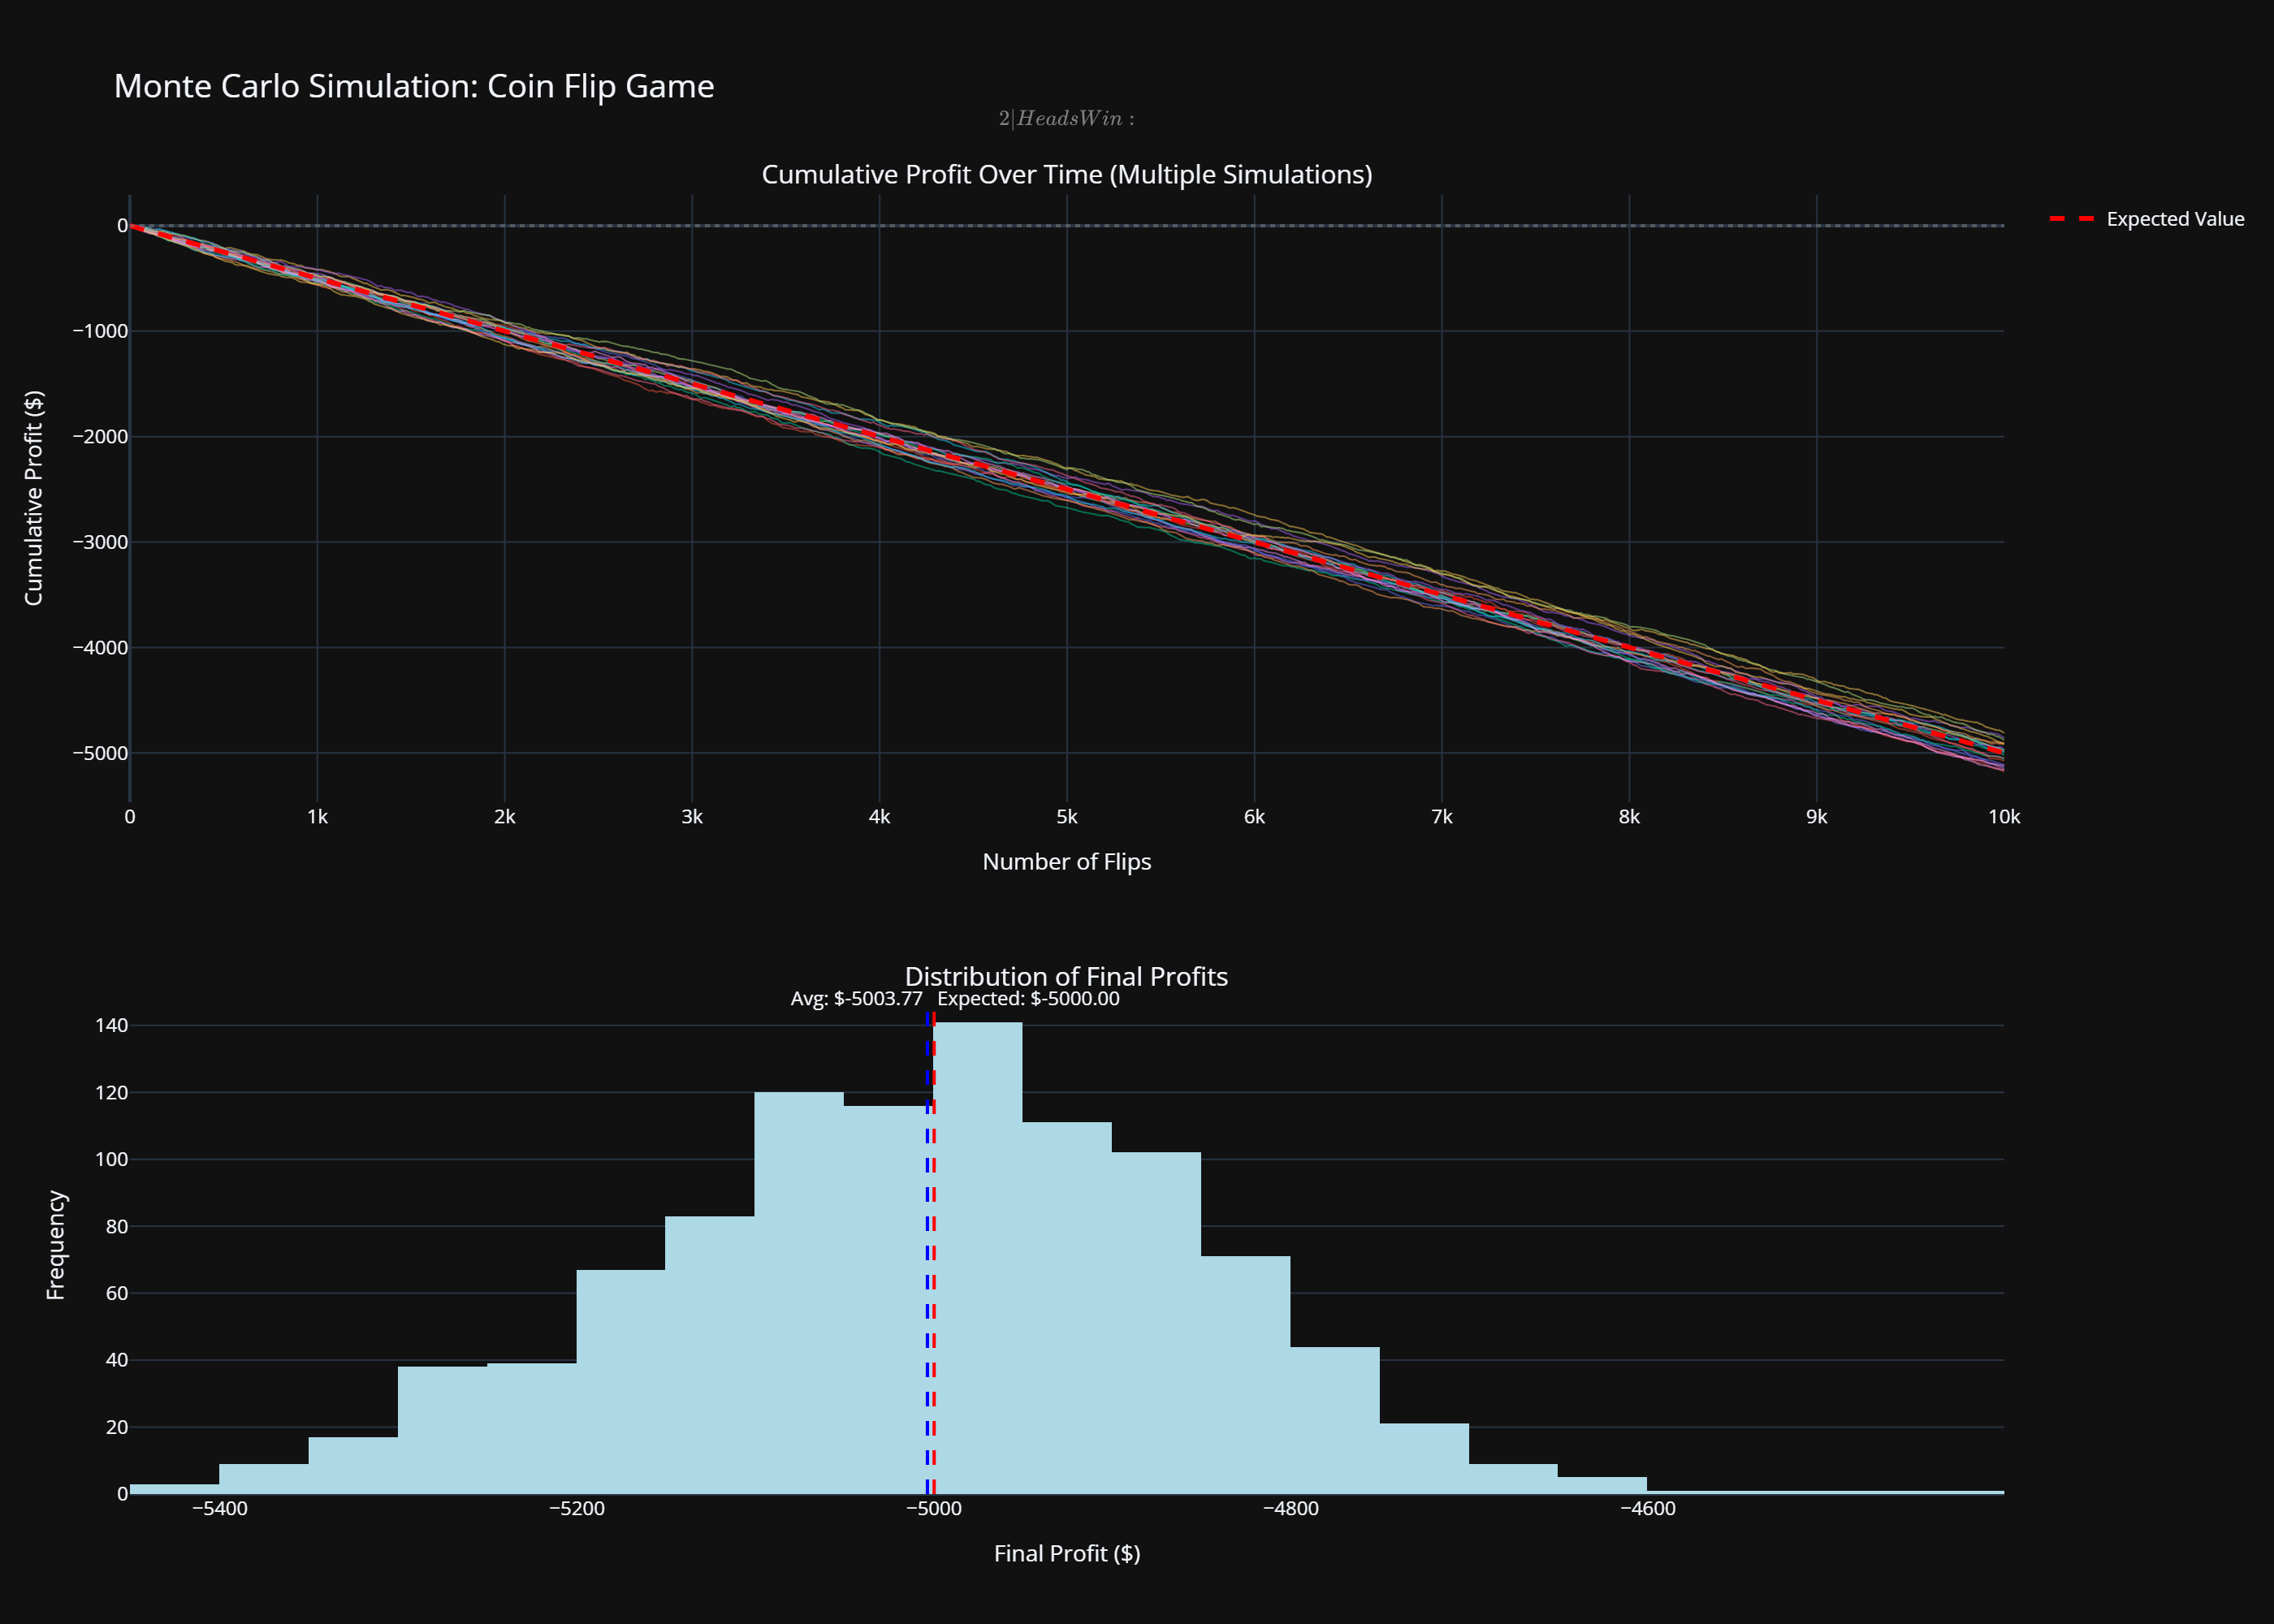
\includegraphics[width=0.8\textwidth]{-ev/10k-ev.png}
\caption{Simulation with 10,000 flips (-EV). The downward trend is absolute.}
\end{figure}

% --- SECTION 4: NEUTRAL EV SIMULATION ---
\section{Case Study 3: The Neutral EV Game (A Random Walk)}
This final case represents a "fair game" where neither the player nor the house has an edge.

\subsection{Game Rules and Calculation}
\begin{itemize}
    \item \textbf{Cost to Play:} \$1.50
    \item \textbf{Heads Payout:} \$3.00 (Net profit: \$1.50)
    \item \textbf{Tails Payout:} \$0.00 (Net loss: \$1.50)
\end{itemize}
The Expected Value per flip is:
\[
EV = (0.5 \times \$1.50) + (0.5 \times -\$1.50) = \$0.75 - \$0.75 = \boldsymbol{\$0.00}
\]
With an EV of zero, there is no long-term upward or downward pressure on the outcome. This is known as a \textbf{Random Walk}.

\subsection{Simulation Results}
In a random walk, the "expected" final position is the starting point (zero profit). However, the variance of the final position grows with time. The paths do not converge; instead, they diffuse outwards. While the average of all simulations will be near zero, any single simulation is likely to wander far from it.

\begin{figure}[h!]
\centering
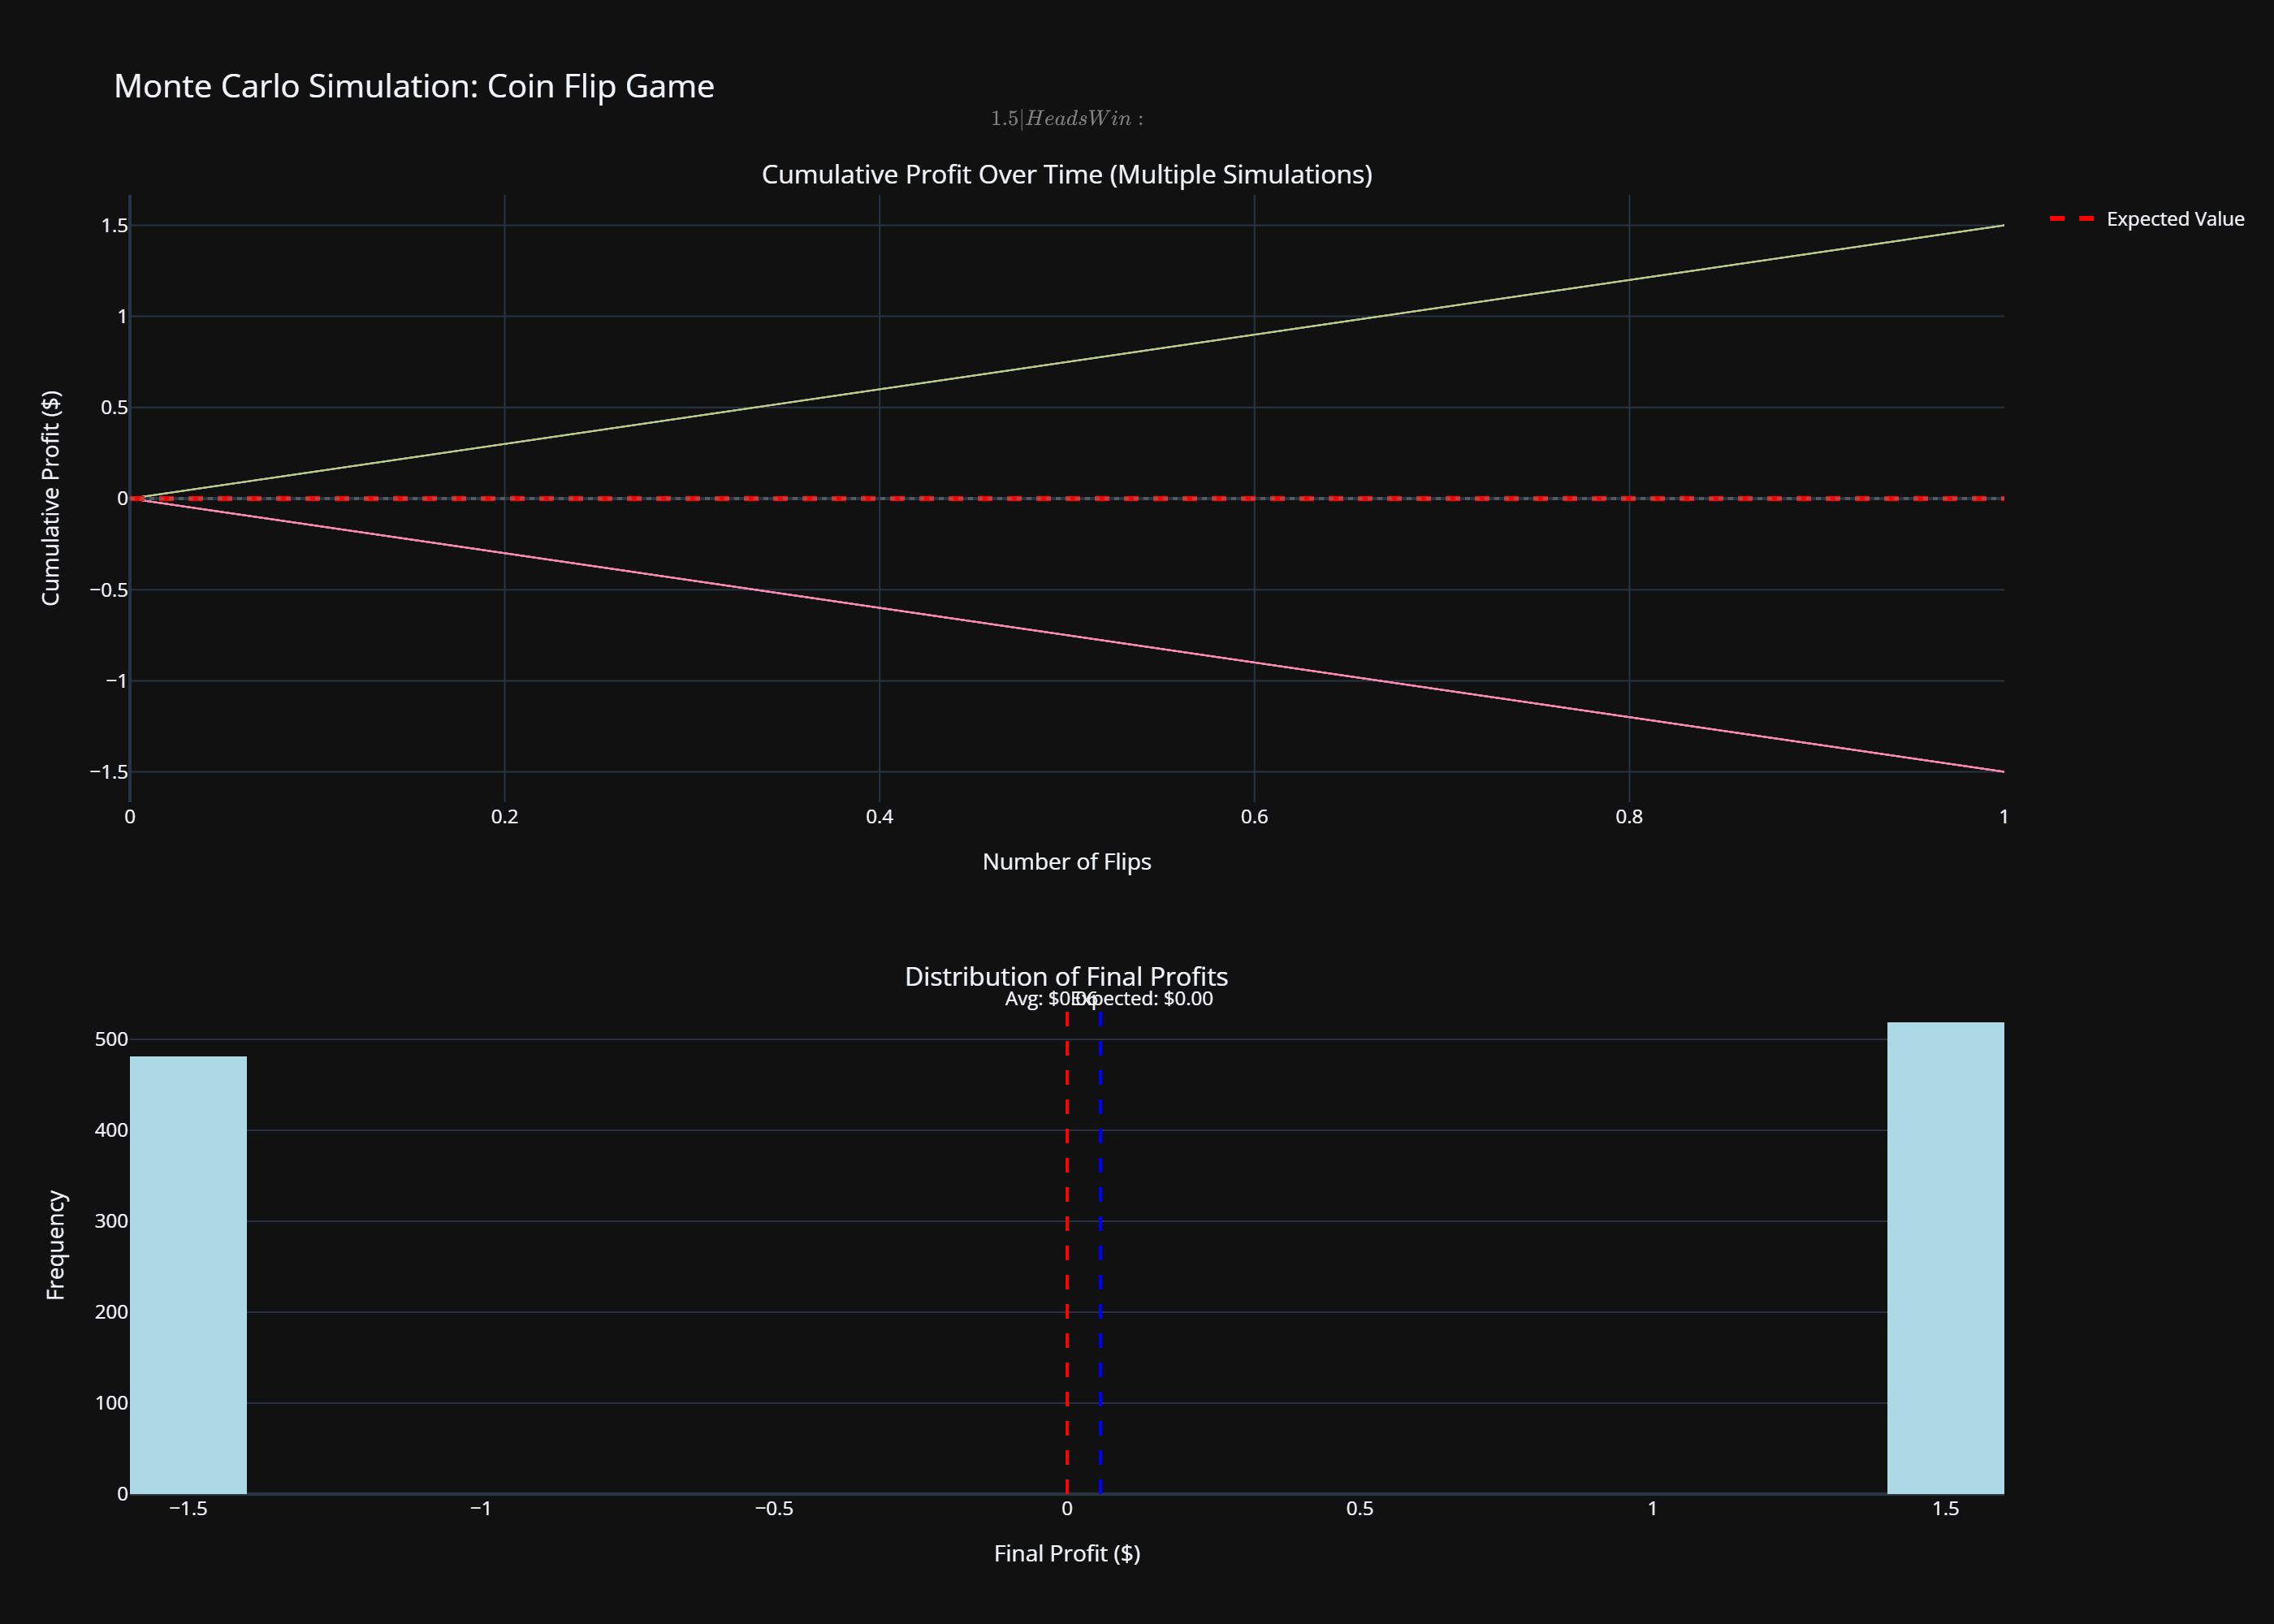
\includegraphics[width=0.8\textwidth]{nev/1nev.png}
\caption{Simulation with 1 flip (0 EV). Outcome is +/-\$1.50.}
\end{figure}

\begin{figure}[h!]
\centering
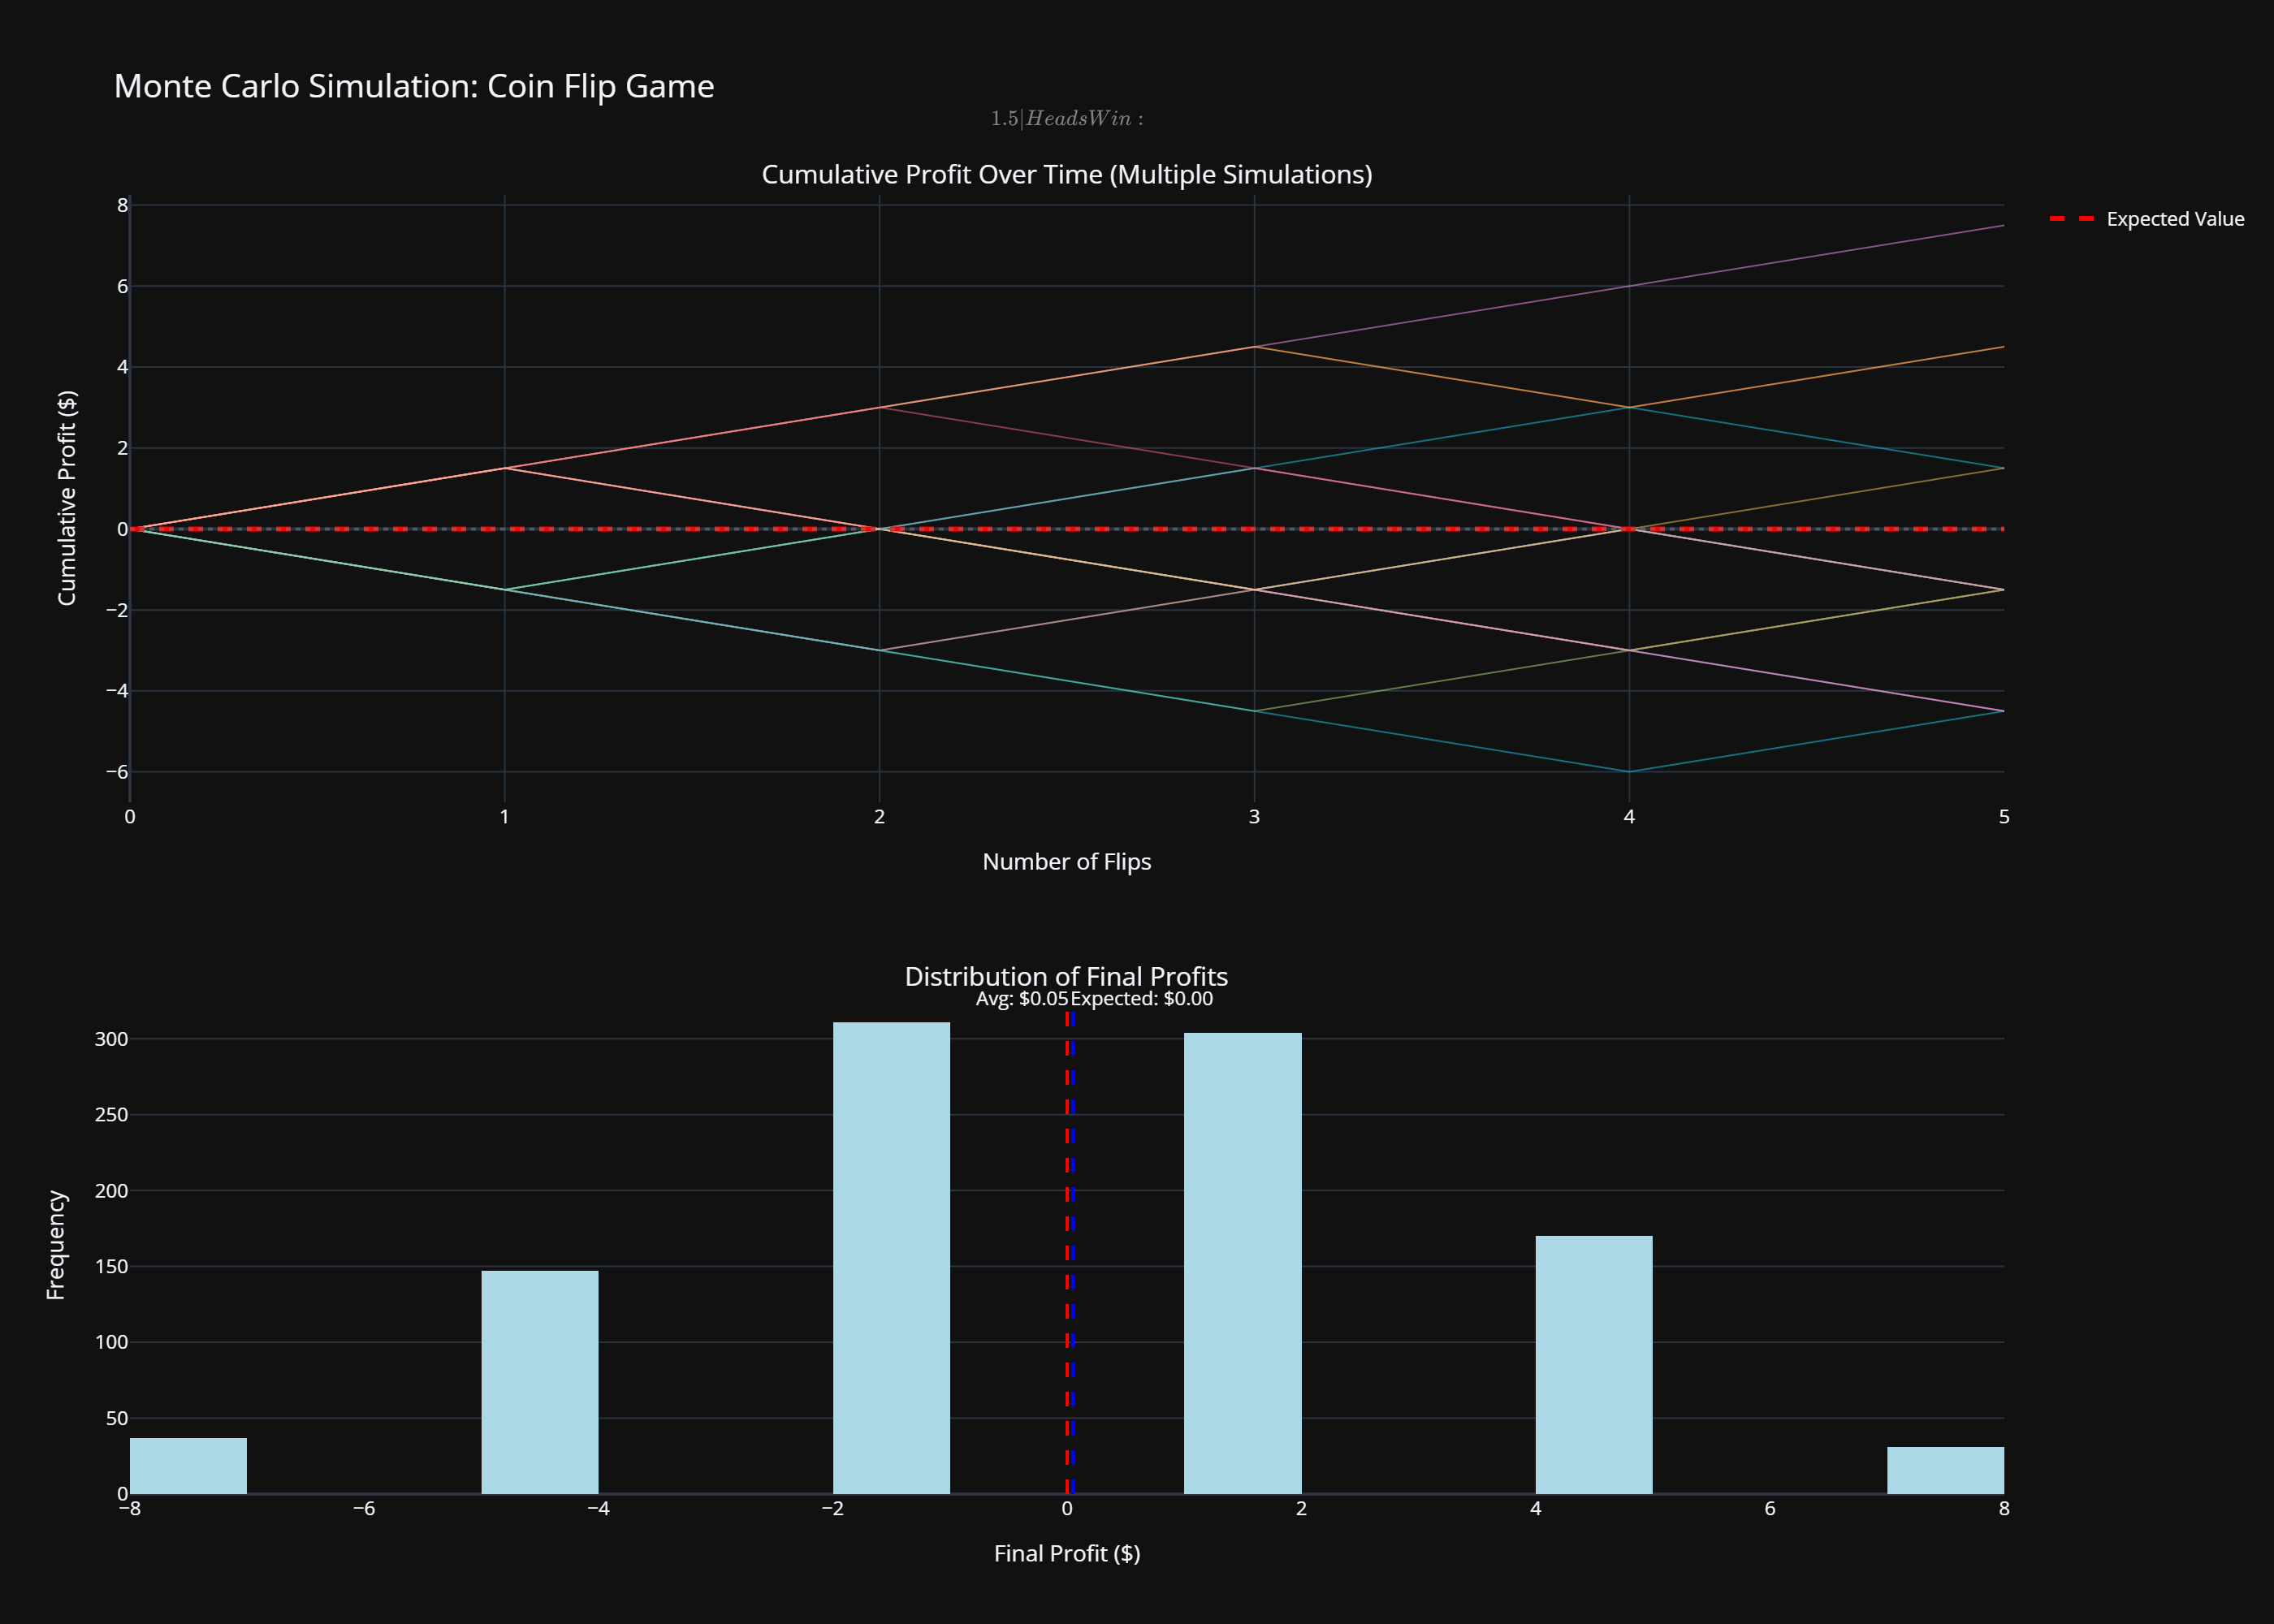
\includegraphics[width=0.8\textwidth]{nev/5nev.png}
\caption{Simulation with 5 flips (0 EV).}
\end{figure}
\clearpage

\begin{figure}[h!]
\centering
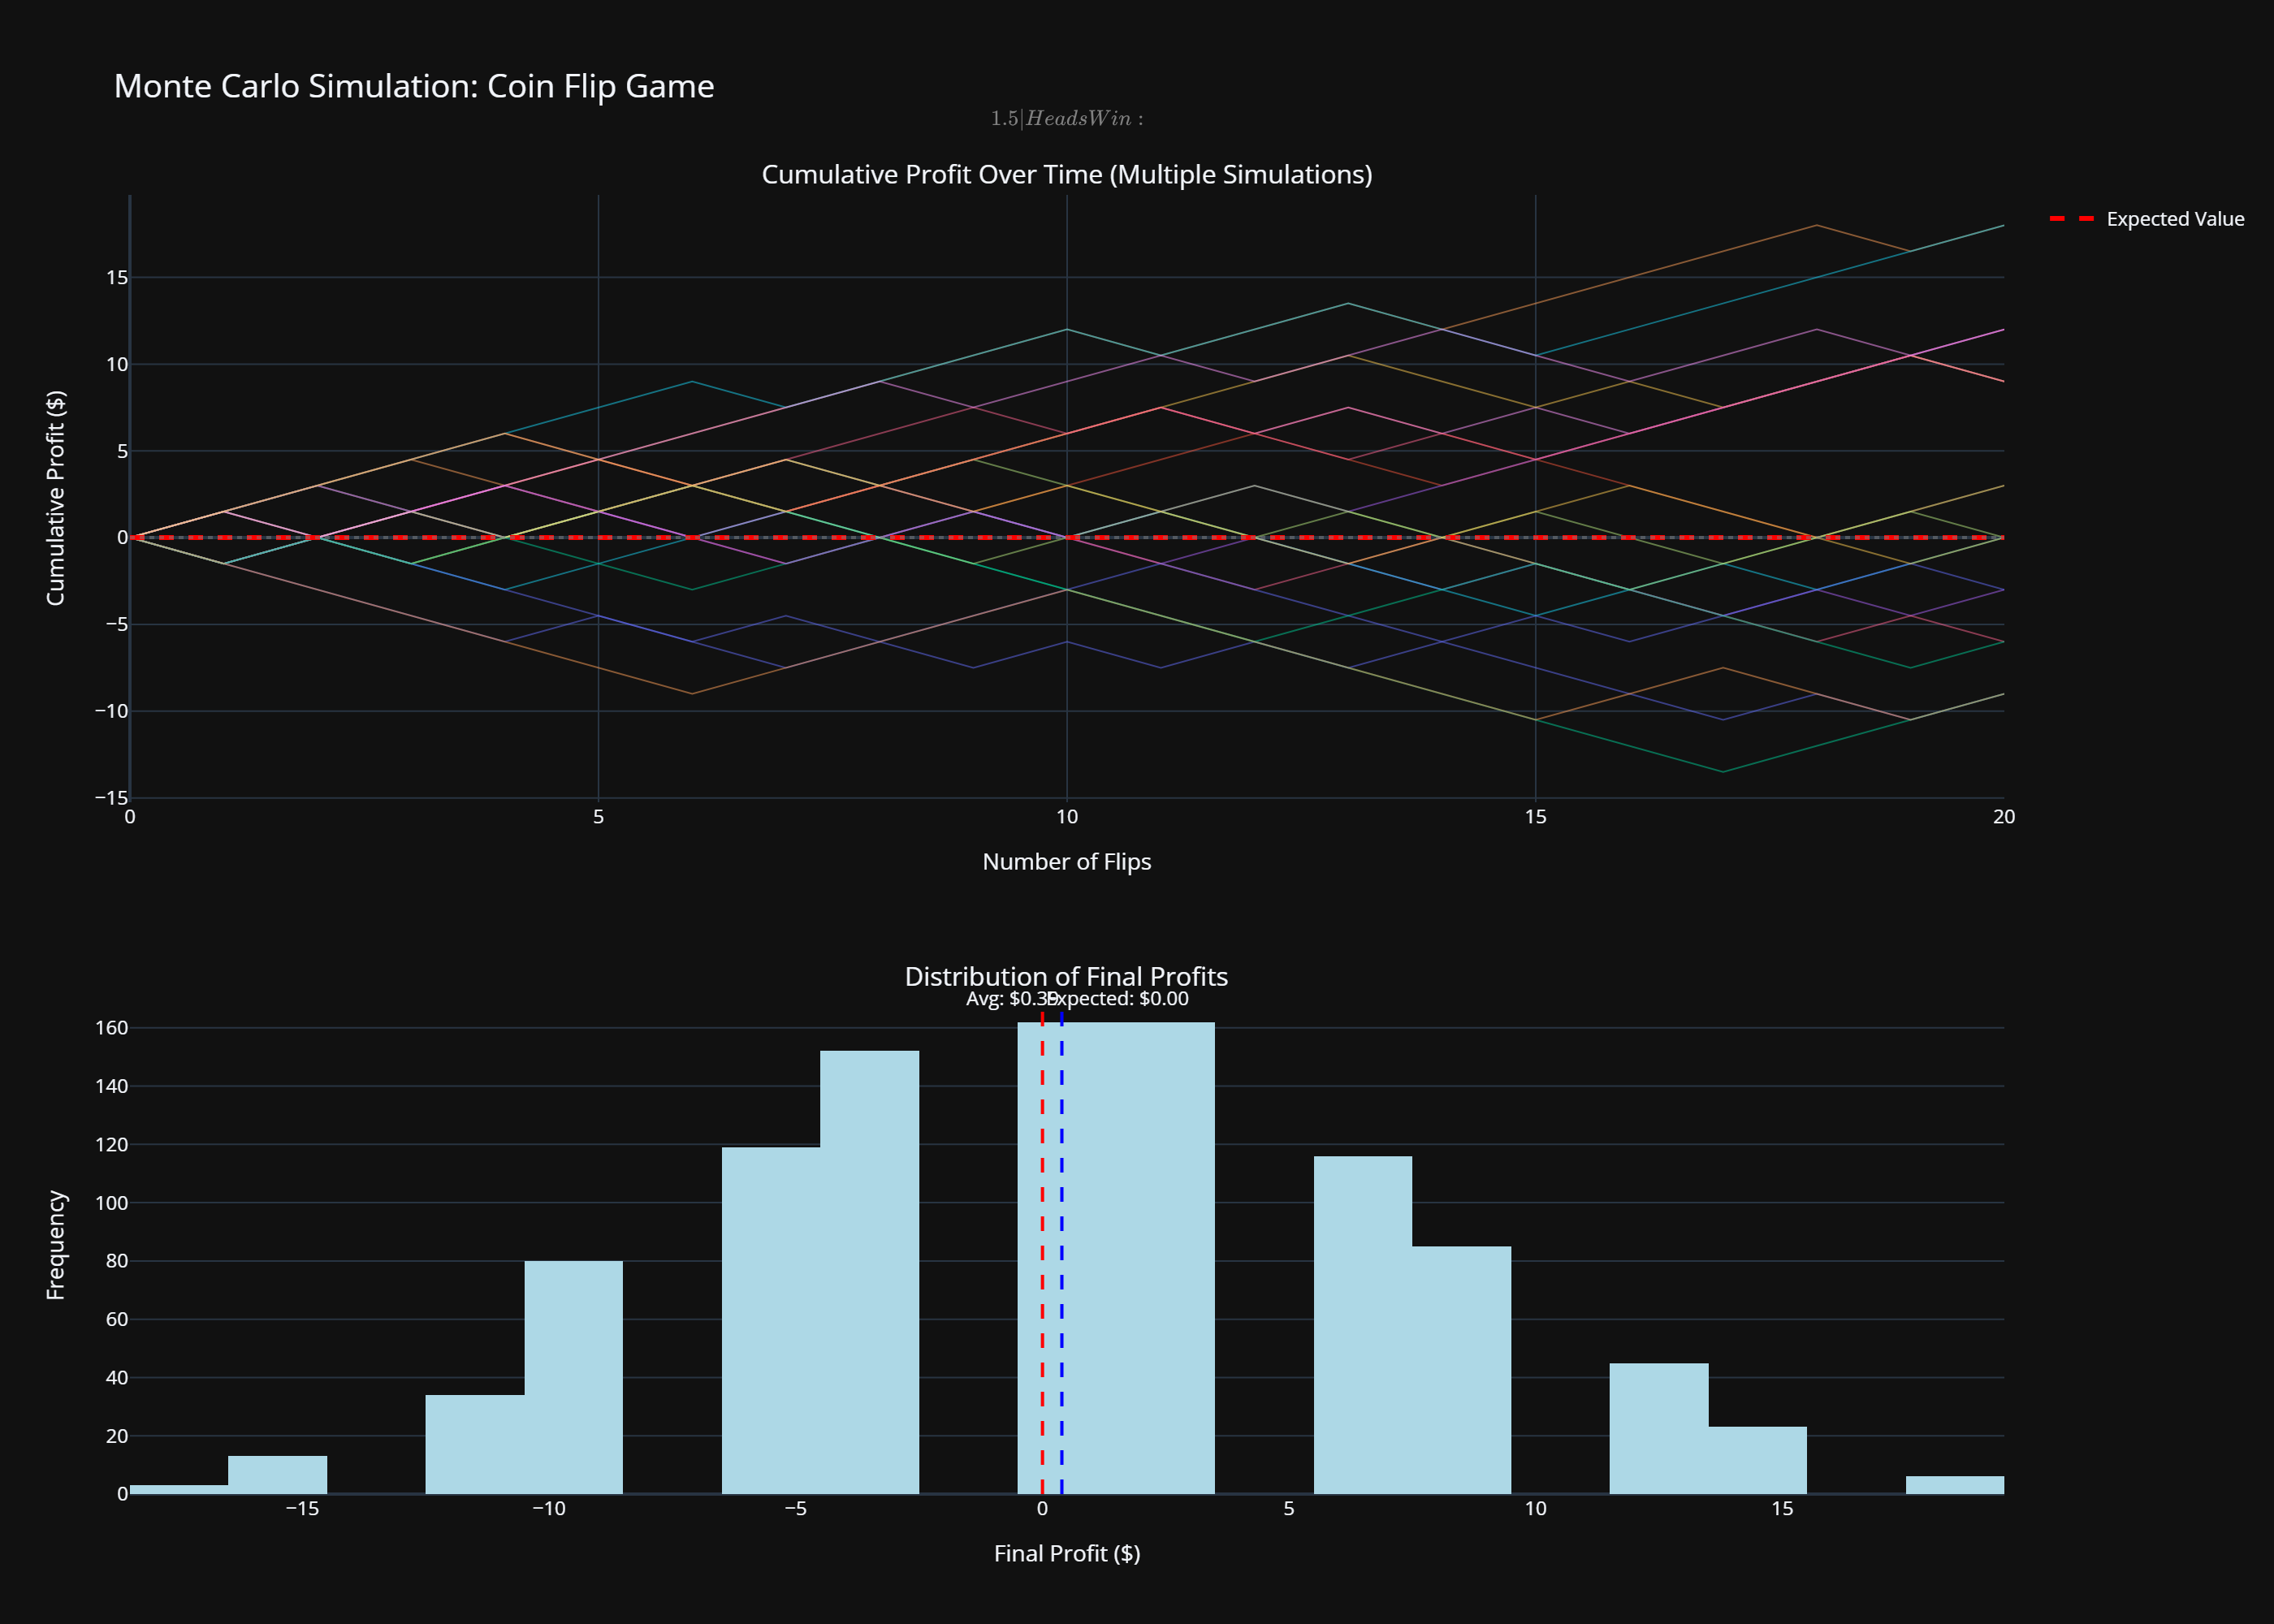
\includegraphics[width=0.8\textwidth]{nev/20nev.png}
\caption{Simulation with 20 flips (0 EV).}
\end{figure}

\begin{figure}[h!]
\centering
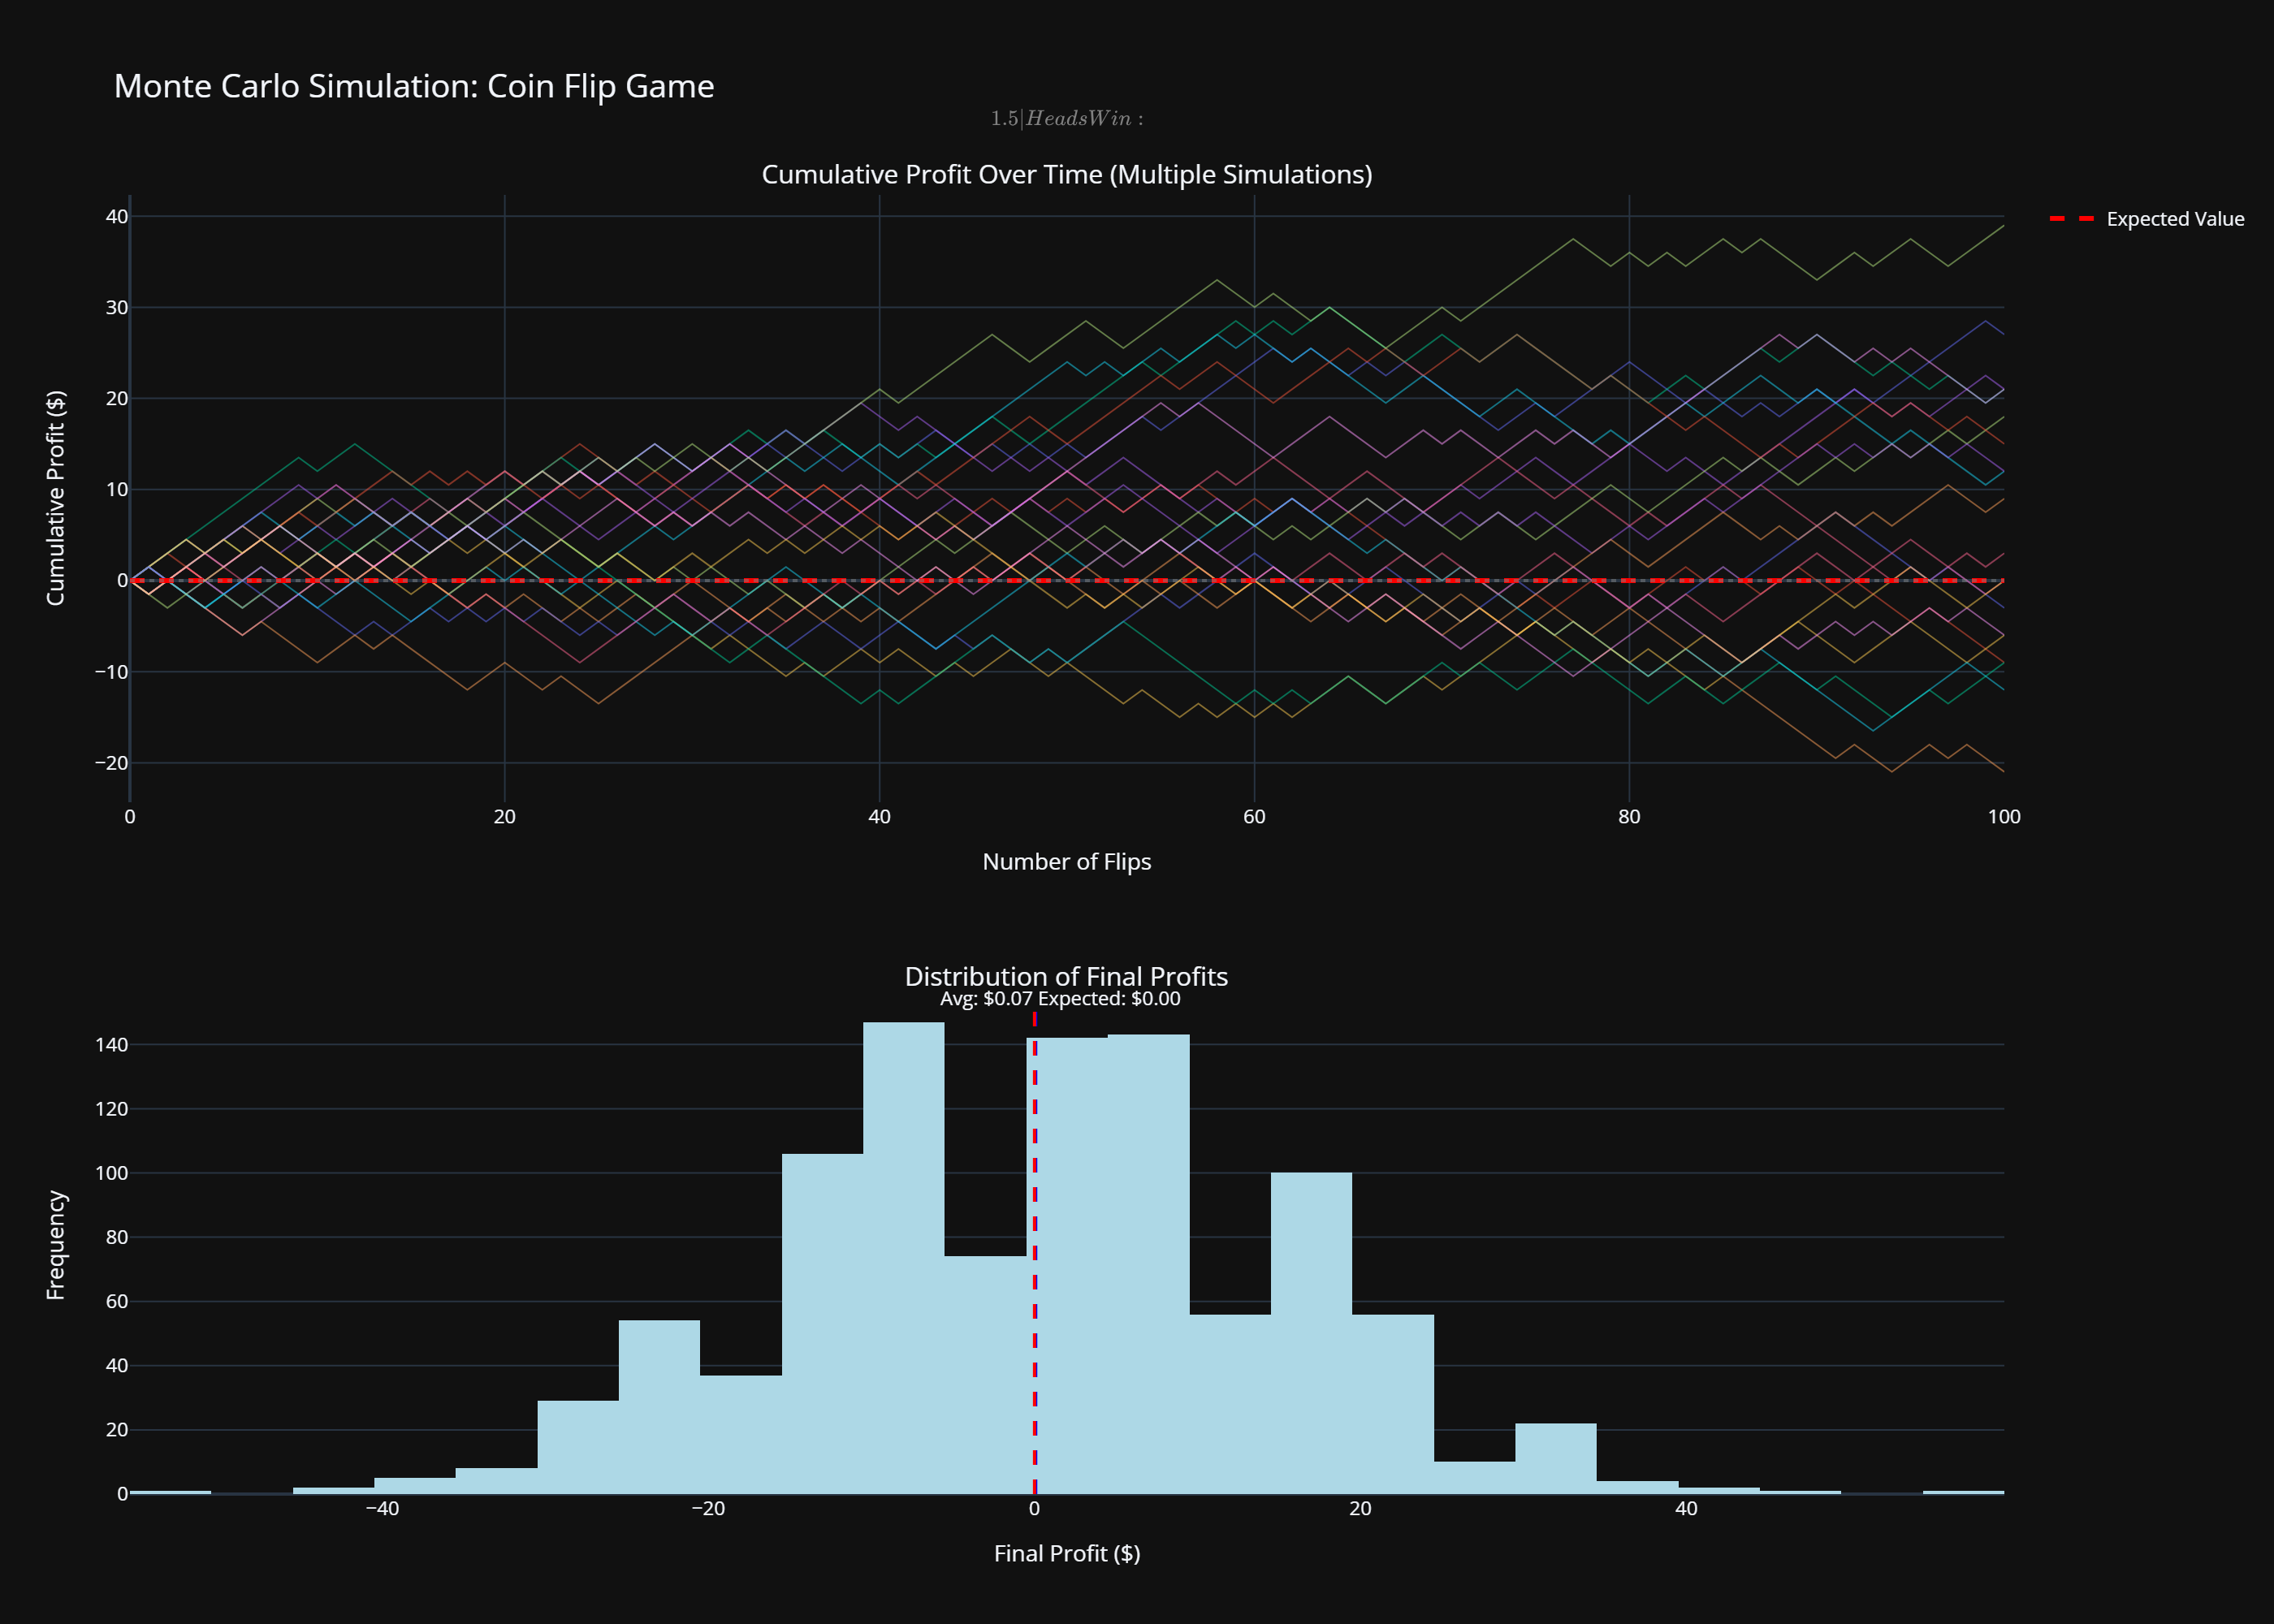
\includegraphics[width=0.8\textwidth]{nev/100nev.png}
\caption{Simulation with 100 flips (0 EV).}
\end{figure}
\clearpage

\begin{figure}[h!]
\centering
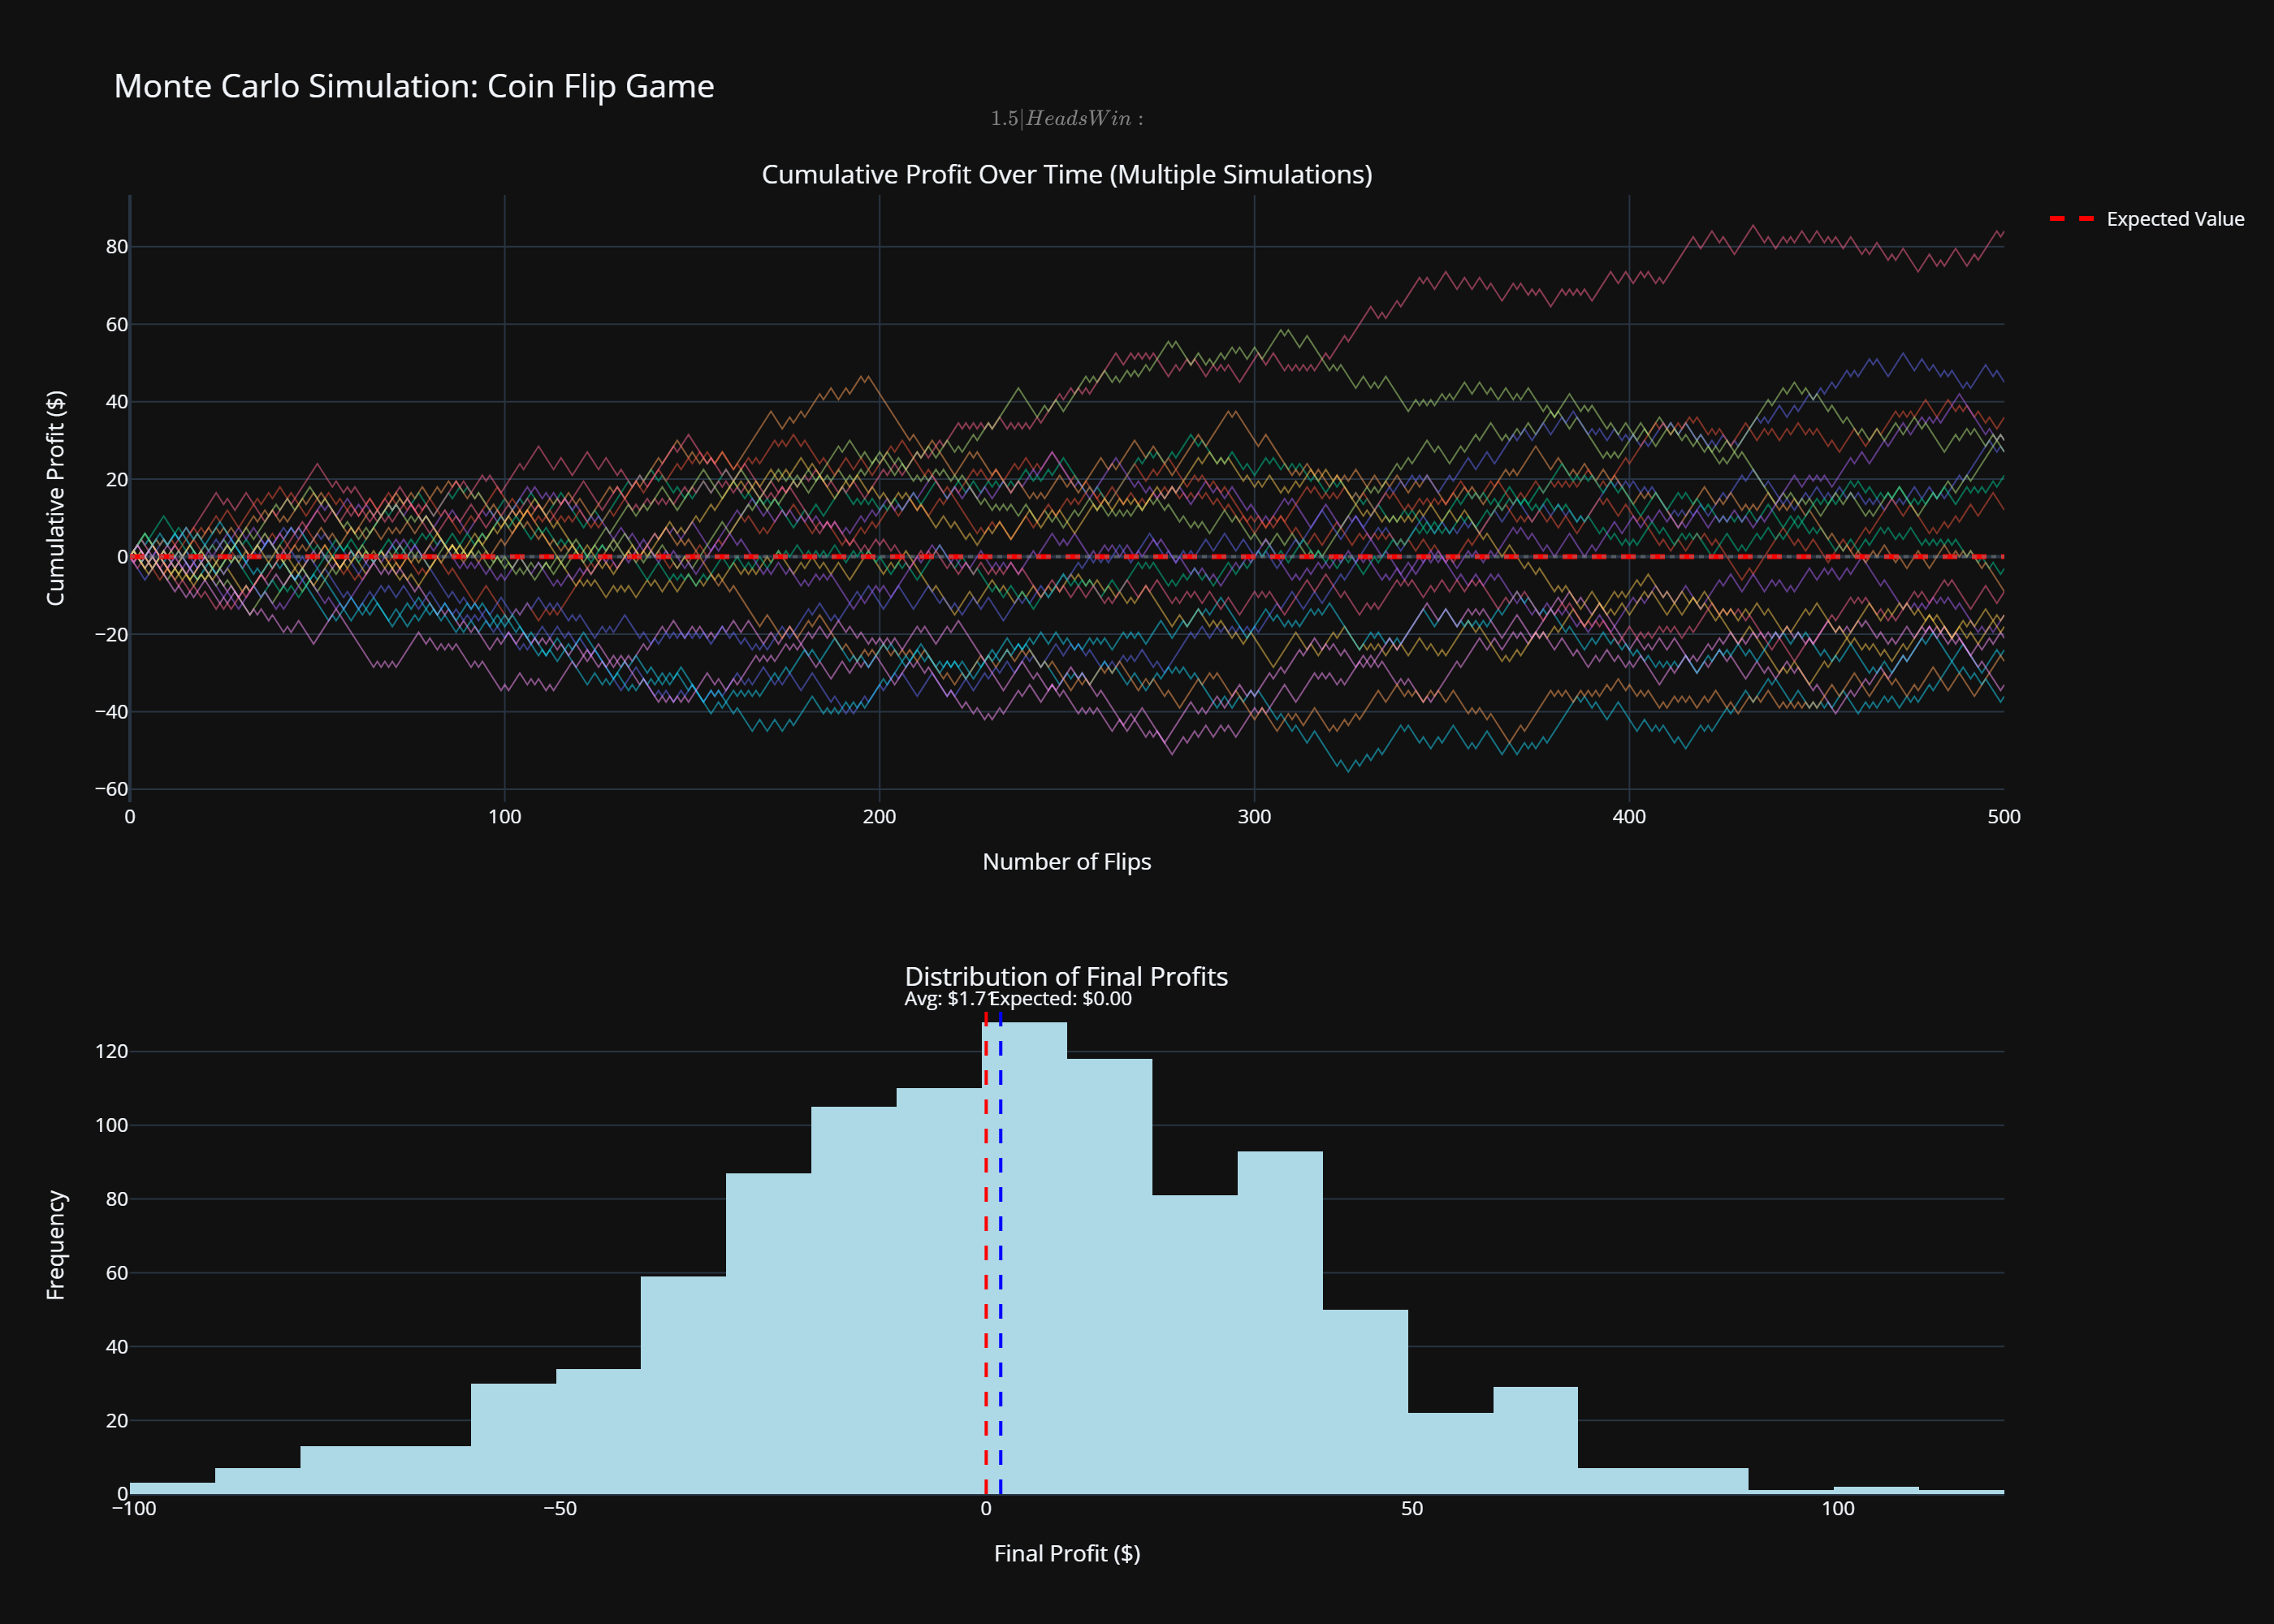
\includegraphics[width=0.8\textwidth]{nev/500nev.png}
\caption{Simulation with 500 flips (0 EV).}
\end{figure}

\begin{figure}[h!]
\centering
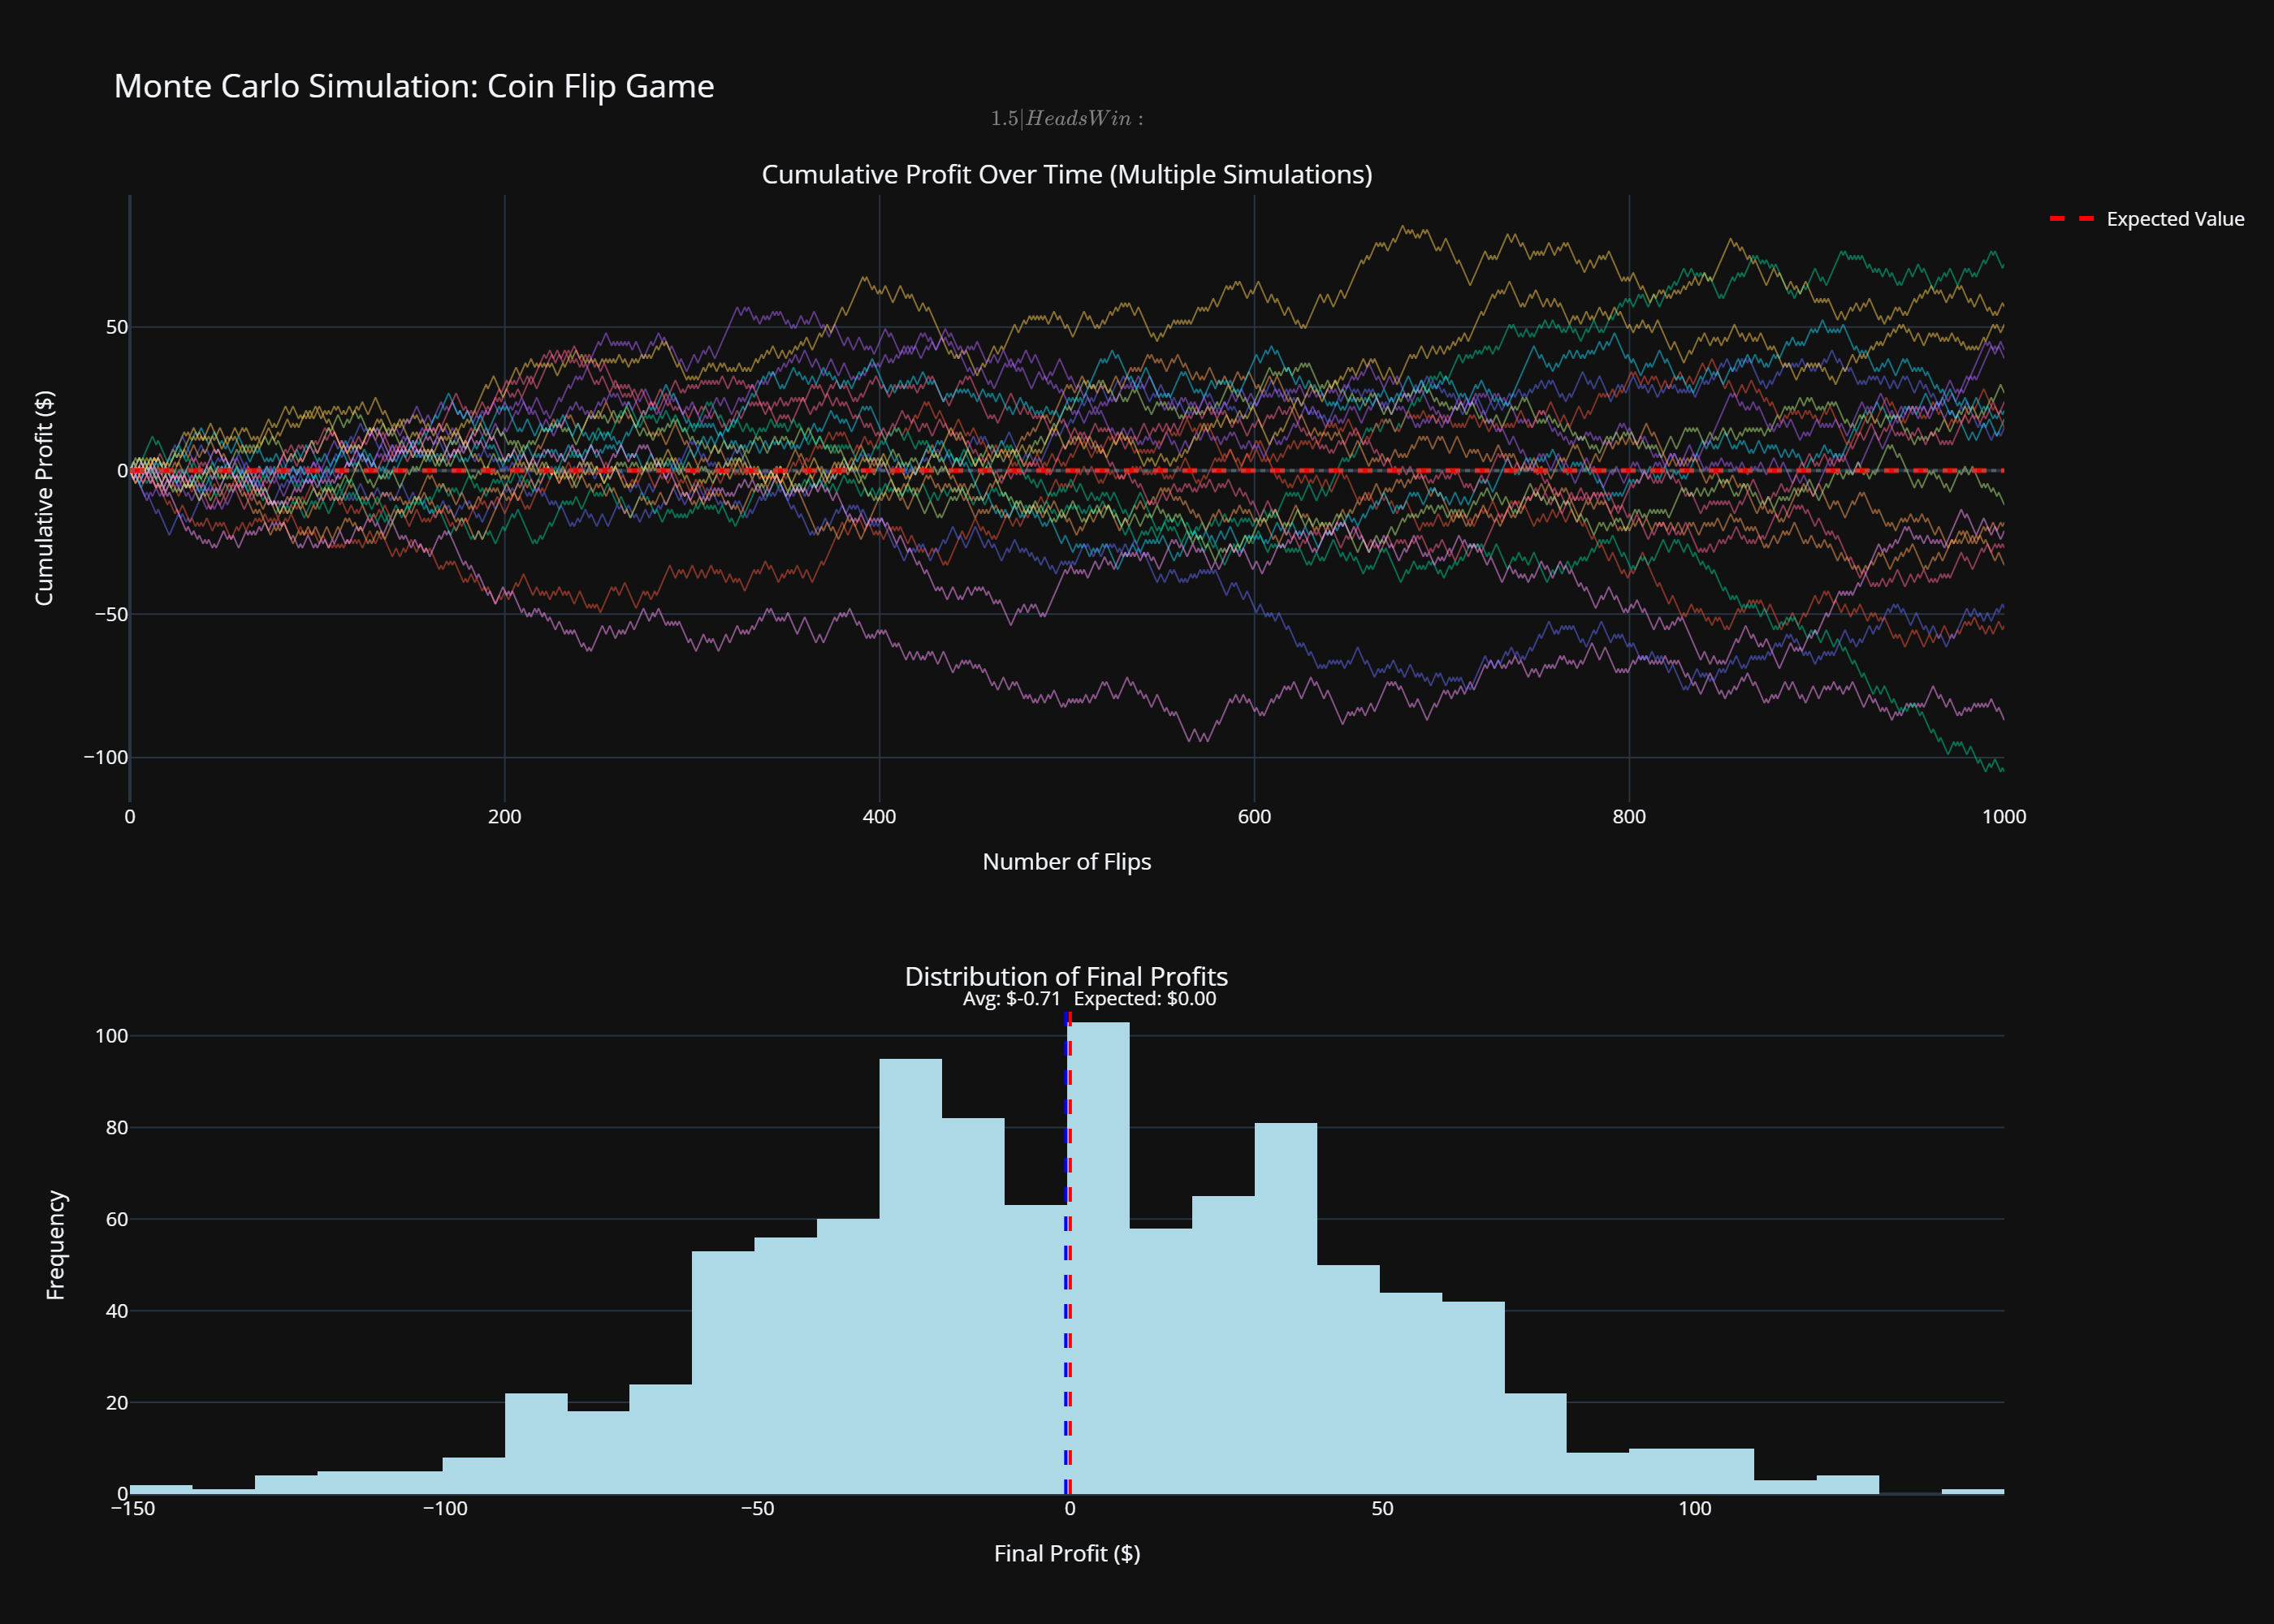
\includegraphics[width=0.8\textwidth]{nev/1000nev.png}
\caption{Simulation with 1,000 flips (0 EV).}
\end{figure}
\clearpage

\begin{figure}[h!]
\centering
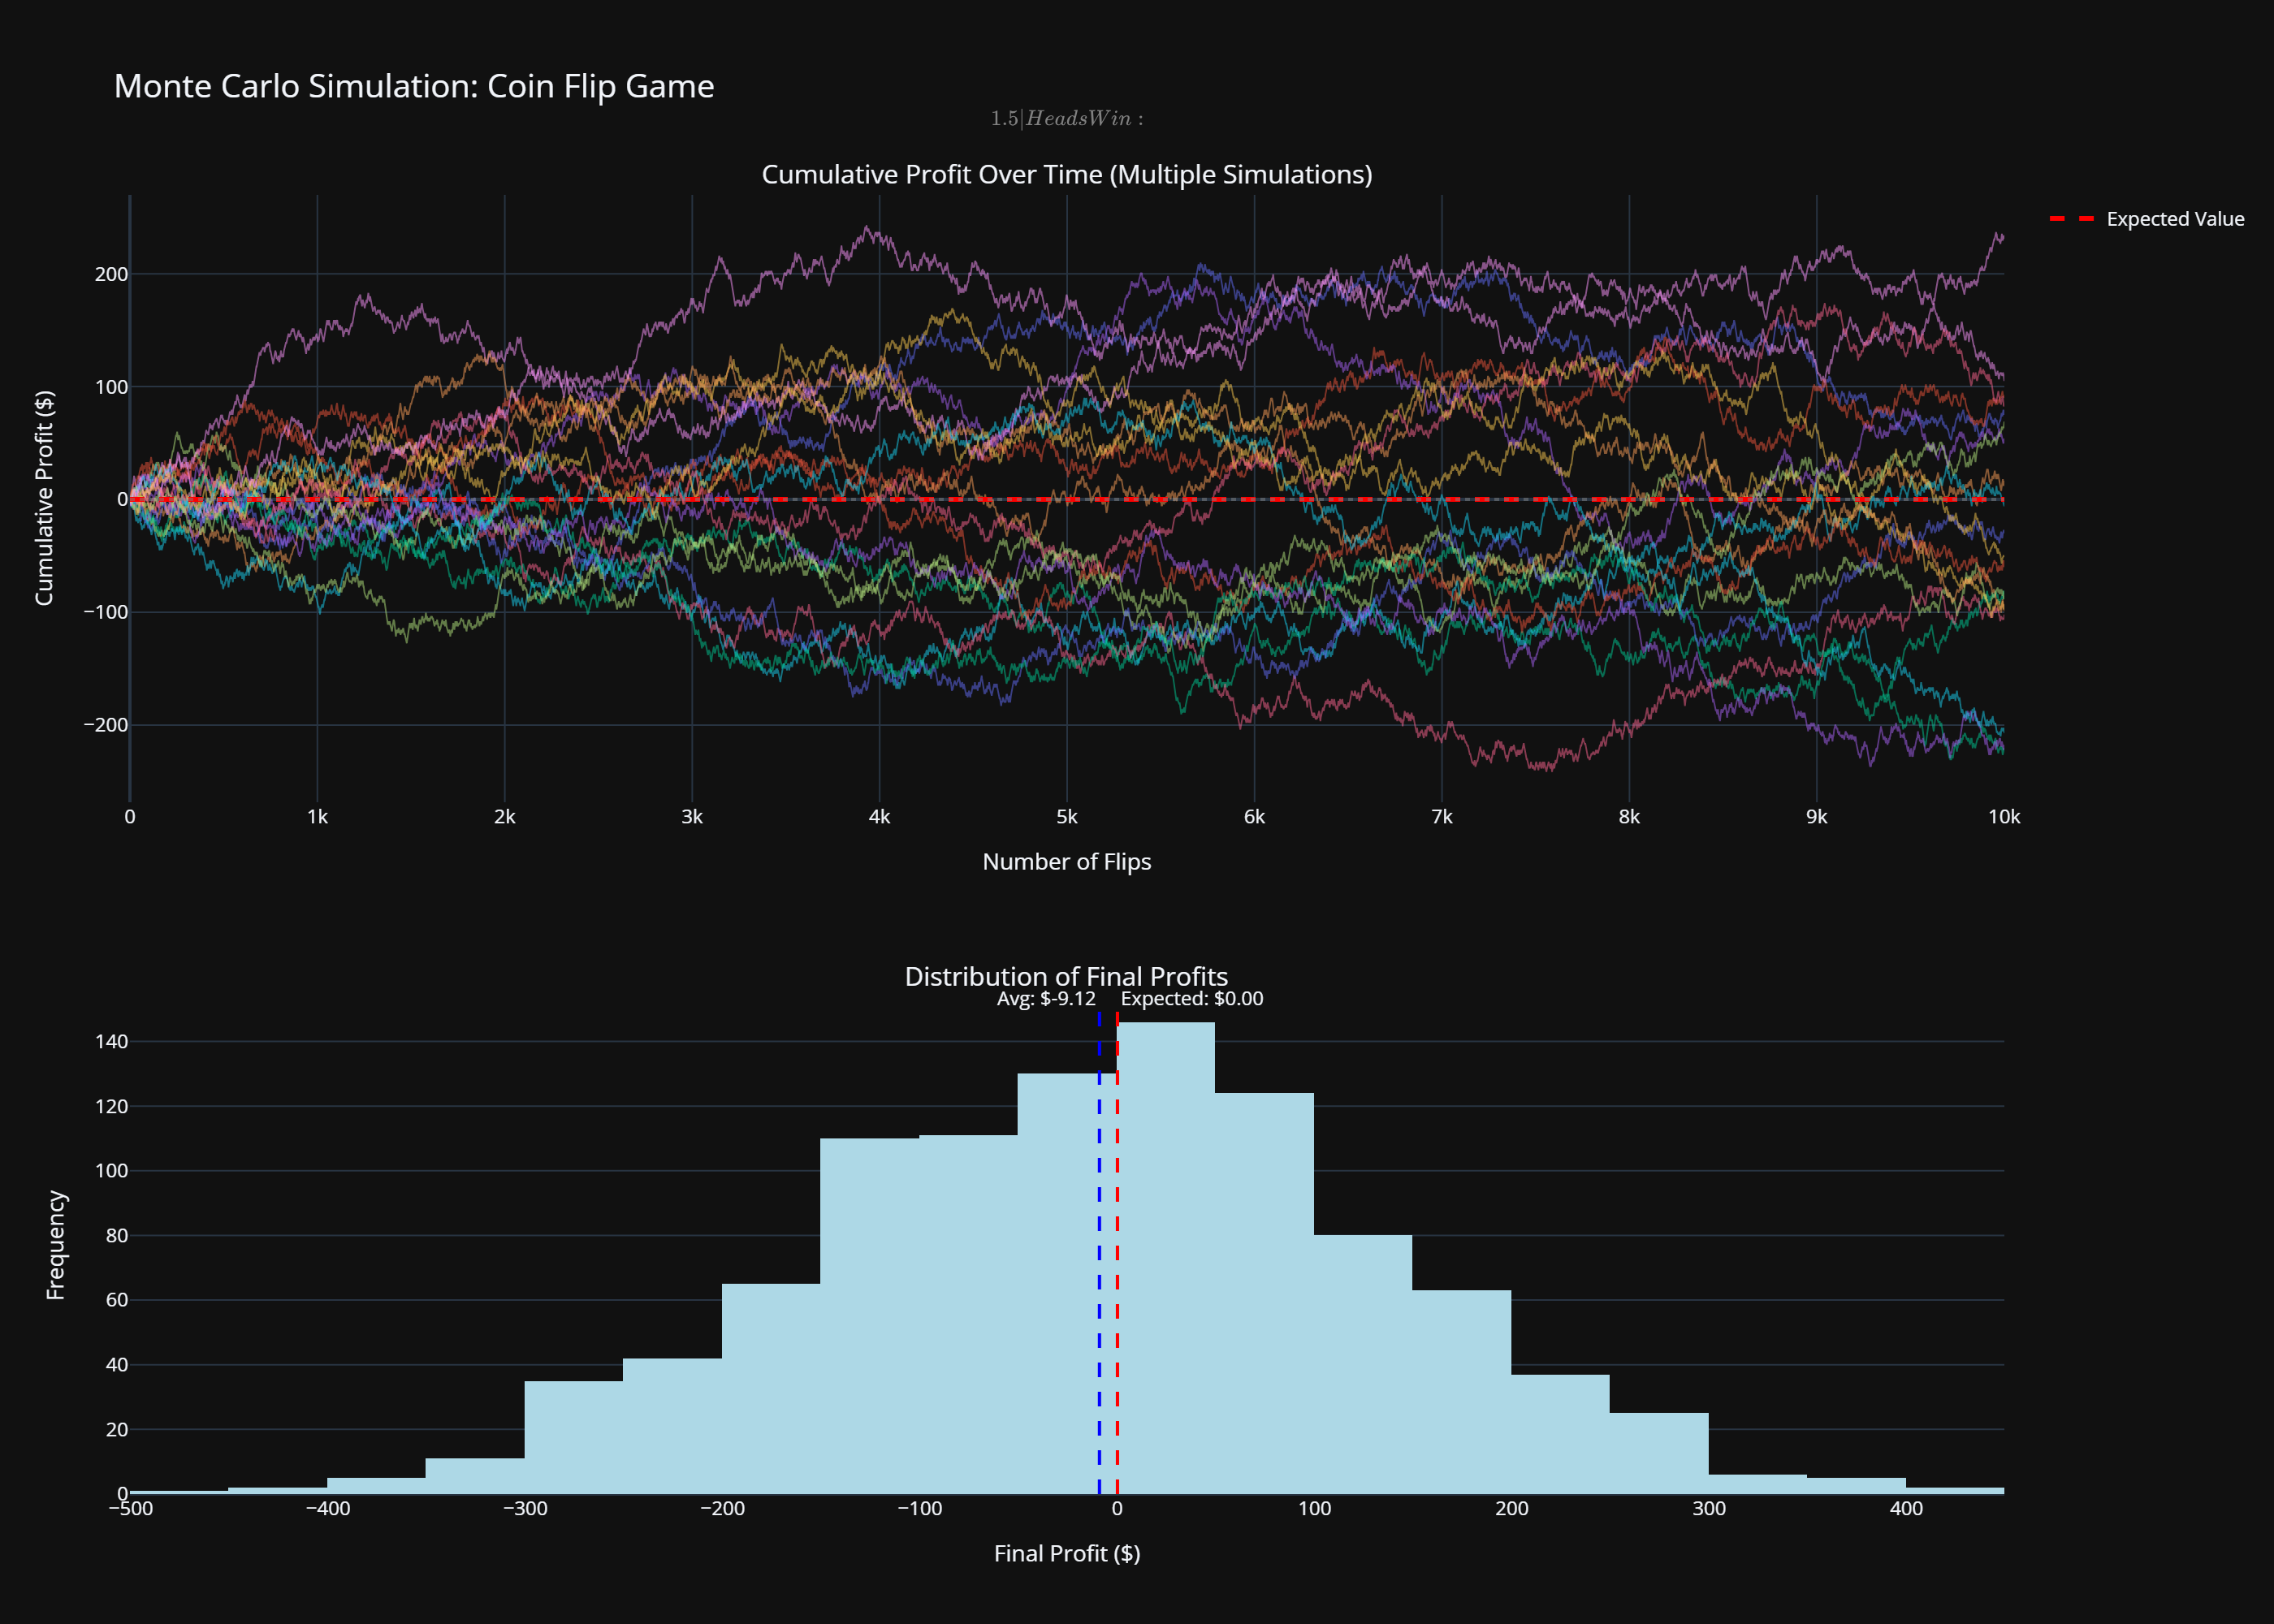
\includegraphics[width=0.8\textwidth]{nev/10knev.png}
\caption{Simulation with 10,000 flips (0 EV). The paths have diffused widely.}
\end{figure}

% --- SECTION 5: CONCLUSION ---
\section{Conclusion}
This series of Monte Carlo simulations has provided a clear, visual confirmation of fundamental statistical laws.

\begin{enumerate}
    \item \textbf{Expected Value dictates the trend.} A positive EV creates a gravitational pull towards profit, while a negative EV ensures long-term loss. A neutral EV results in an aimless random walk.
    \item \textbf{The Law of Large Numbers ensures convergence.} For games with a non-zero EV, the LLN guarantees that the average outcome will approach this EV as the number of trials increases. This is because the variance of the average profit, $\sigma^2/n$, shrinks towards zero.
    \item \textbf{Sample size is paramount.} In the short term, variance dominates and outcomes are unpredictable. In the long term, the underlying EV dominates and outcomes become highly predictable. This is the crucial transition from gambling (low $n$) to statistical certainty (high $n$).
\end{enumerate}

Ultimately, these simulations prove that while individual events are random, the aggregate behavior of a large number of them is not. It is governed by the mathematical structure of the system, and with enough data, the random noise fades to reveal a deterministic trend.

% --- SECTION 6: REAL-WORLD APPLICATIONS ---
\section{Real-World Applications: From Poker to Wall Street}

The principles demonstrated in our coin-flip simulation are not merely academic; they are the mathematical foundation upon which fortunes are built in fields that manage probabilistic outcomes.

\subsection{The Professional Poker Player}
A common misconception is that poker is a game of luck. While short-term results are heavily influenced by chance (\textit{variance}), long-term success is determined by skill. This skill is, fundamentally, the ability to consistently make decisions with a positive Expected Value.

When a professional player decides whether to call, bet, or fold, they are intuitively (or mathematically) calculating the EV of that decision. They assess:
\begin{itemize}
    \item \textbf{Pot Odds:} The ratio of the current size of the pot to the cost of a contemplated call.
    - \textbf{Equity:} The player's probability of winning the hand against their opponent's likely range of hands.
\end{itemize}

\begin{itemize}
    \item \textbf{A Single Hand as a Single Flip:} A pro can make a perfect +EV decision but still lose the hand due to a "bad beat." This is the same as our +EV game resulting in a loss on a single flip (tails).
    \item \textbf{The Law of Large Numbers in Action:} Profitability is realized over thousands of hands. Over a large sample size, the effects of short-term luck are smoothed out, and the player's underlying statistical edge (their skill) prevails, leading to consistent profit.
    \item \textbf{Bankroll Management as Variance Control:} A professional's bankroll is their tool to withstand variance. It must be large enough to absorb the inevitable downswings (losing streaks) so they can continue playing long enough for their +EV decisions to yield the expected returns.
\end{itemize}

\subsection{The Quantitative Trader}
Quantitative trading firms use algorithmic strategies to execute millions of trades per day. Many of these strategies are built on finding a small, persistent statistical edge with a positive Expected Value.

The "edge," or \textit{alpha}, might be minuscule. For example a high-frequency trading strategy might have an EV of a fraction of a cent per share traded. On a single trade, this edge is meaningless and swamped by market noise (\texttit{variance}).

However, the strategy's power comes from the enormous number of trials.
\begin{itemize}
    \item \textbf{A Single Trade as a Single Flip:} A single trade can easily lose money.
    \item \textbf{The Law of Large Numbers at Scale:} By executing millions or billions of trades, the LLN ensures that the tiny positive EV will translate into substantial and highly predictable profits. The sheer volume of trades allows the statistical edge to overcome the randomness of the market.
    \item \textbf{Risk Management as Variance Control:} Just like a poker player's bankroll, quant firms use sophisticated risk management models. They control position sizes and set stop-losses to ensure that a string of bad outcomes (\textit{variance}) does not wipe out their capital, allowing them to operate long enough for their statistical edge to materialize.
\end{itemize}

In both poker and quantitative finance, the core principle is the same: find an edge (a +EV scenario) and repeat it enough times for the Law of Large Numbers to guarantee a profitable result.


\clearpage
\appendix
\section{Python Simulation Code}

The following Python code was used to run the Monte Carlo simulations discussed in this paper. It requires the `numpy` and `plotly` libraries.

\begin{lstlisting}[language=Python, caption={Monte Carlo Simulation Script}, label={code:simulation}]
import numpy as np
import plotly.graph_objects as go
from plotly.subplots import make_subplots
import os
from datetime import datetime

COST = 1.5
PAYOUT_HEADS = 3
PAYOUT_TAILS = 0
EV = (0.5 * PAYOUT_HEADS) + (0.5 * PAYOUT_TAILS) - COST
NUM_FLIPS = 5
NUM_SIMULATIONS = 1000

def simulate_coin_flips(n_flips):
    flips = np.random.randint(0, 2, n_flips)
    profits = np.where(flips == 1, PAYOUT_HEADS - COST, -COST)
    cumulative_profit = np.cumsum(profits)
    return cumulative_profit

print(f"Running {NUM_SIMULATIONS} simulations with {NUM_FLIPS} flips each...")
all_simulations = []
final_profits = []

for i in range(NUM_SIMULATIONS):
    cumulative_profit = simulate_coin_flips(NUM_FLIPS)
    all_simulations.append(cumulative_profit)
    final_profits.append(cumulative_profit[-1])

all_simulations = np.array(all_simulations)
final_profits = np.array(final_profits)

avg_final_profit = np.mean(final_profits)
theoretical_profit = EV * NUM_FLIPS
profitable_sims = np.sum(final_profits > 0)
profit_percentage = (profitable_sims / NUM_SIMULATIONS) * 100

print(f"\n{'='*60}")
print(f"RESULTS:")
print(f"{'='*60}")
print(f"Expected Value per flip: ${EV:.2f}")
print(f"Theoretical profit after {NUM_FLIPS} flips: ${theoretical_profit:.2f}")
print(f"Average profit across all simulations: ${avg_final_profit:.2f}")
print(f"Profitable simulations: {profitable_sims}/{NUM_SIMULATIONS} ({profit_percentage:.1f}%)")
print(f"Min profit: ${np.min(final_profits):.2f}")
print(f"Max profit: ${np.max(final_profits):.2f}")
print(f"{'='*60}\n")

fig = make_subplots(
    rows=2, cols=1,
    subplot_titles=(
        'Cumulative Profit Over Time (Multiple Simulations)',
        'Distribution of Final Profits'
    ),
    vertical_spacing=0.15,
    row_heights=[0.55, 0.45]
)

num_to_plot = min(20, NUM_SIMULATIONS)
x_values = np.arange(1, NUM_FLIPS + 1)

for i in range(num_to_plot):
    y_with_start = np.concatenate([[0], all_simulations[i]])
    x_with_start = np.concatenate([[0], x_values])

    fig.add_trace(
        go.Scatter(
            x=x_with_start,
            y=y_with_start,
            mode='lines',
            name=f'Sim {i+1}',
            line=dict(width=1),
            opacity=0.5,
            showlegend=False
        ),
        row=1, col=1
    )

# ev line starting from 0
theoretical_x = np.concatenate([[0], x_values])
theoretical_y = EV * theoretical_x

fig.add_trace(
    go.Scatter(
        x=theoretical_x,
        y=theoretical_y,
        mode='lines',
        name='Expected Value',
        line=dict(color='red', width=3, dash='dash'),
        showlegend=True
    ),
    row=1, col=1
)

fig.add_hline(y=0, line_dash="dot", line_color="gray", opacity=0.5, row=1, col=1)

fig.add_trace(
    go.Histogram(
        x=final_profits,
        nbinsx=30,
        name='Final Profits',
        marker_color='lightblue',
        showlegend=False
    ),
    row=2, col=1
)

#avoiding overlap
fig.add_vline(
    x=avg_final_profit,
    line_dash="dash",
    line_color="blue",
    annotation_text=f"Avg: ${avg_final_profit:.2f}",
    annotation_position="top left",
    annotation_yshift=10,
    row=2, col=1
)

fig.add_vline(
    x=theoretical_profit,
    line_dash="dash",
    line_color="red",
    annotation_text=f"Expected: ${theoretical_profit:.2f}",
    annotation_position="top right",
    annotation_yshift=10,
    row=2, col=1
)

fig.update_xaxes(title_text="Number of Flips", row=1, col=1)
fig.update_yaxes(title_text="Cumulative Profit ($)", row=1, col=1)
fig.update_xaxes(title_text="Final Profit ($)", row=2, col=1)
fig.update_yaxes(title_text="Frequency", row=2, col=1)

fig.update_layout(
    height=1000,
    title_text=f"Monte Carlo Simulation: Coin Flip Game",
    title_font_size=20,
    showlegend=True,
    hovermode='closest',
    font=dict(size=12),
    margin=dict(t=120, b=80, l=80, r=80)
)

fig.add_annotation(
    text=f"Cost: ${COST} | Heads Win: ${PAYOUT_HEADS} | EV: ${EV:.2f}/flip | {NUM_SIMULATIONS} simulations × {NUM_FLIPS} flips",
    xref="paper", yref="paper",
    x=0.5, y=1.05,
    xanchor='center', yanchor='bottom',
    showarrow=False,
    font=dict(size=13, color="gray")
)

timestamp = datetime.now().strftime("%Y%m%d_%H%M%S")
output_filename = f"coin_flip_simulation_{timestamp}.png"

try:
    print(f"Exporting plot to {output_filename}...")
    fig.write_image(output_filename, width=1400, height=1000, scale=2)
    print(f"✓ Plot saved successfully to {os.path.abspath(output_filename)}")
except PermissionError:
    print(f"✗ Permission denied. The file might be open in another program.")
    print(f"  Trying alternative filename...")
    alt_filename = f"coin_flip_sim_{timestamp}_alt.png"
    try:
        fig.write_image(alt_filename, width=1400, height=1000, scale=2)
        print(f"✓ Plot saved to {os.path.abspath(alt_filename)}")
    except Exception as e:
        print(f"✗ Could not save file: {e}")
except Exception as e:
    print(f"✗ Error saving image: {e}")

fig.show()
\end{lstlisting}
\end{document}